\documentclass{article}

\usepackage{geometry}

\geometry{a4paper}

% \usepackage[UTF8, heading = false, scheme = plain]{ctex}%格式

% \usepackage{ctex}

%\usepackage{authblk} %添加机构 安装preprint后可用

\usepackage{graphicx} %添加图片
\usepackage{listings}
\usepackage{float}  %设置图片浮动位置的宏包
\usepackage{subfigure}  %插入多图时用子图显示的宏包
\usepackage{amsthm}
\usepackage{booktabs}       % professional-quality tables
\usepackage{amsfonts}       % blackboard math symbols
\usepackage{nicefrac}       % compact symbols for 1/2, etc.
\usepackage{microtype}      % microtypography
\usepackage{multirow}
\usepackage{caption}
\usepackage{times}
% \usepackage{subcaption}
% \usepackage{fontspec} % 定制字体

\usepackage{xcolor} % 定制颜色
\definecolor{mygreen}{rgb}{0,0.6,0}
\definecolor{mygray}{rgb}{0.5,0.5,0.5}
\definecolor{mymauve}{rgb}{0.58,0,0.82}
\lstset{ %
backgroundcolor=\color{white},      % choose the background color
basicstyle=\footnotesize\ttfamily,  % size of fonts used for the code
columns=fullflexible,
tabsize=4,
breaklines=true,               % automatic line breaking only at whitespace
captionpos=b,                  % sets the caption-position to bottom
commentstyle=\color{mygreen},  % comment style
escapeinside={\%*}{*},        % if you want to add LaTeX within your code
keywordstyle=\color{blue},     % keyword style
stringstyle=\color{mymauve}\ttfamily,  % string literal style
frame=single,
rulesepcolor=\color{red!20!green!20!blue!20},
% identifierstyle=\color{red},
language=python,
}


\usepackage{amsmath}

\renewcommand{\vec}[1]{\boldsymbol{#1}} % 生产粗体向量,而不是带箭头的向量
\renewcommand{\thesubfigure}{(\arabic{subfigure})}
\usepackage{amssymb}

\usepackage{booktabs} % excel导出的大表格

\usepackage{hyperref}

%\newtheorem{definition}{Definition} %英文
% \setCJKmainfont{hk4e_zh-cn.ttf}     % 语义和语法同fontspec
% \setCJKsansfont{hk4e_zh-cn.ttf}
% \setCJKmonofont{hk4e_zh-cn.ttf}
% \setmainfont{Times New Roman}
% \setsansfont{hk4e_zh-cn.ttf}
% \setmonofont{hk4e_zh-cn.ttf}
%\newtheorem{theorem}{Theorem}
\geometry{a4paper,scale=0.8}
% \newtheorem{definition}{定义} %中文

% \newtheorem{lemma}{引理}

% \newtheorem{theorem}{定理}

%\newenvironment{proof}{{\noindent\it 证明}\quad}{\hfill □ \square□\par}

\DeclareMathOperator{\Ima}{Im}%定义新符号

\DeclareMathOperator{\Rank}{rank}%定义求秩算子

\title{Machine Learning Personal Project}

\author{Jiang Shuyang \\ Email: \href{mailto:jiangshuyang@sjtu.edu.cn}{jiangshuyang@sjtu.edu.cn}}

%\affil{中国科学院} 
%需要把上面的\usepackage{authblk}取消注释

%date{}

\begin{document}

\maketitle

\section{Introduction}
In this project, I finish the basic task, i.e., image classification on MNIST dataset. Besieds, I also finish image generation with VAE and sentiment analysis with LSTM. I will in detail illustrate the model architectures in each task, final result on test set and corresponding visualization results.



\begin{figure}[htbp]
    \centering
    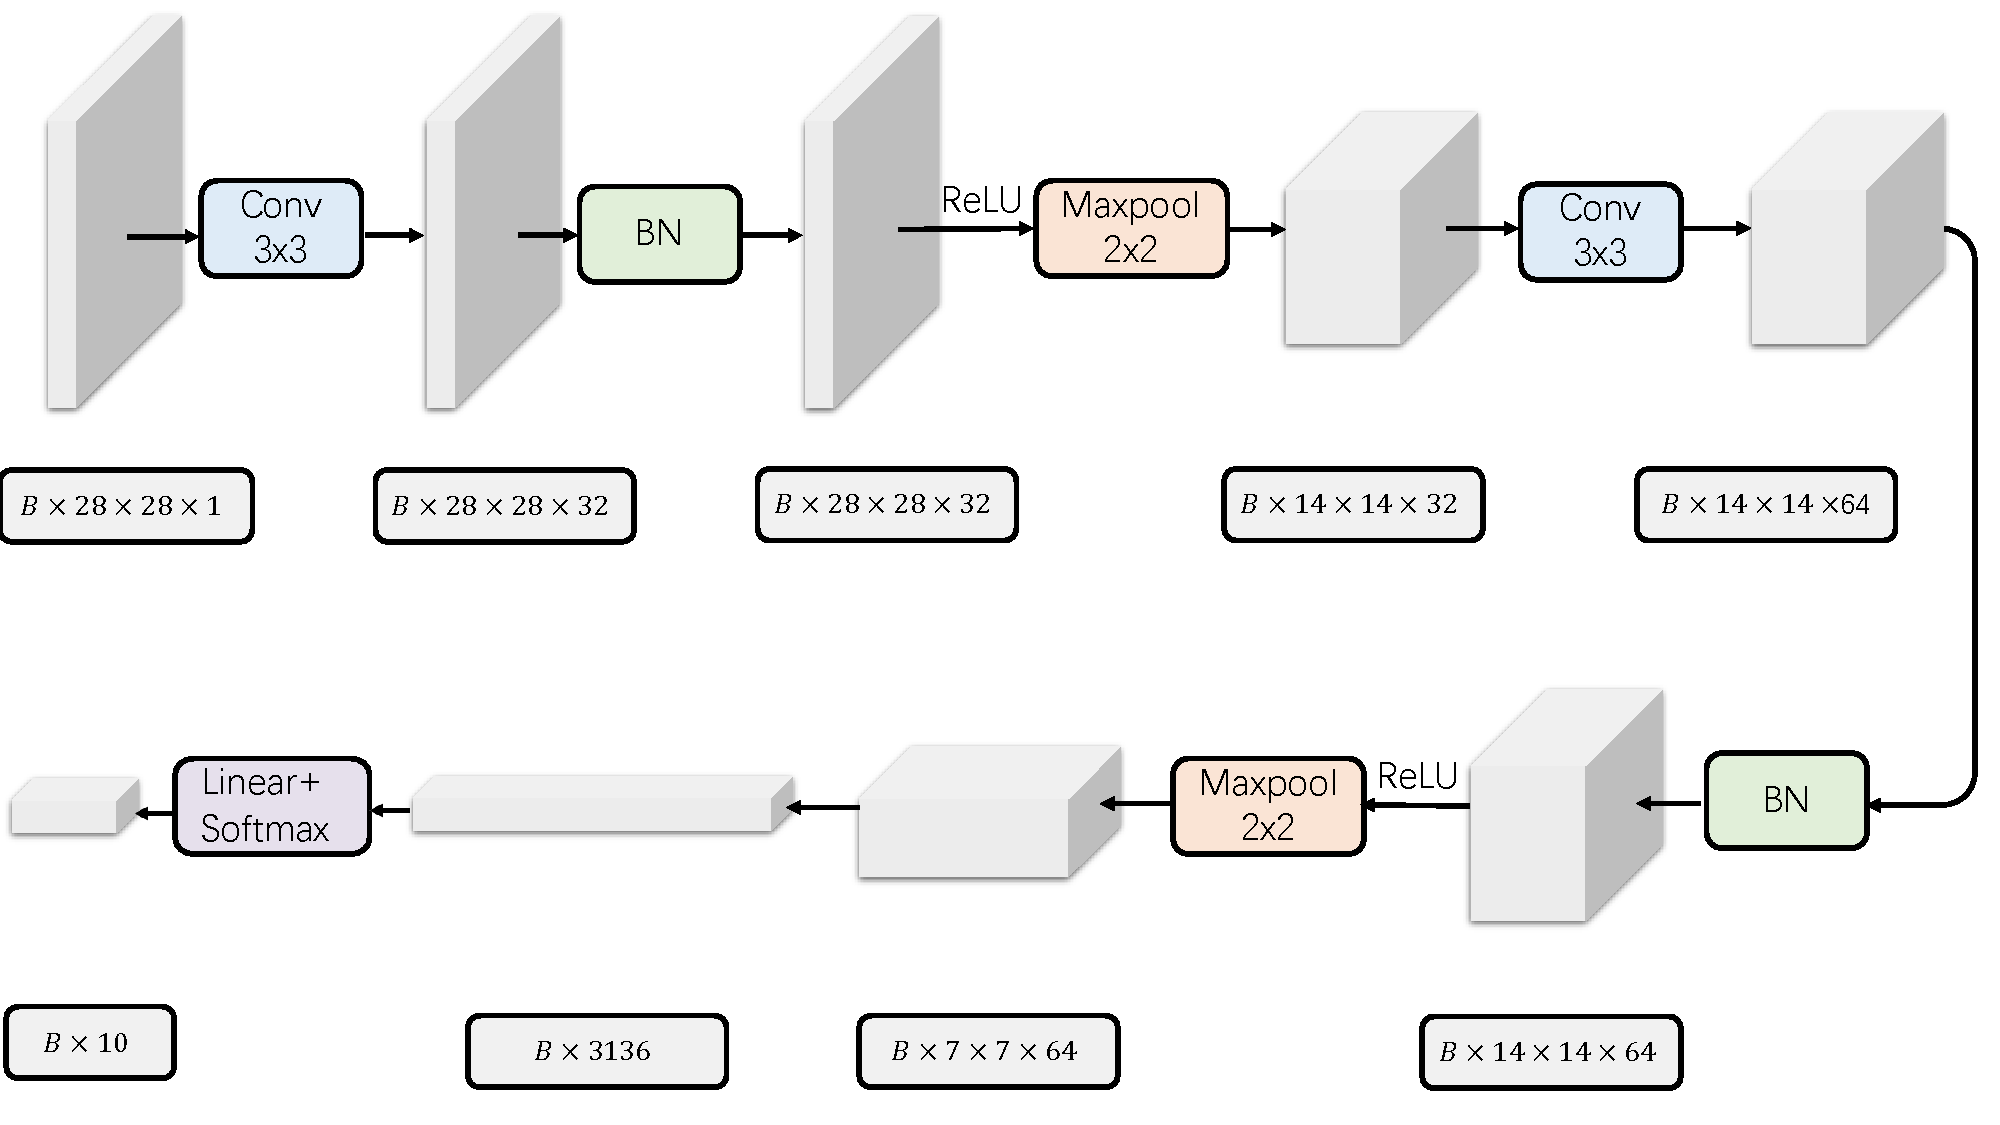
\includegraphics[width=0.8\textwidth]{cnn.pdf}
    \caption{Model diagram of self-designed CNN network for MNIST image classification task. The whole model contains 12 neural layers including the output layer. $B$ stands for the size of a batch.}
    \label{fig:CNN_arch}
\end{figure}

\begin{figure}[htbp]
    \centering
    \includegraphics[width=0.9\textwidth]{../images/mnist-train-loss-acc.png}
    \caption{Training loss and accuracy change figures. The left figure corresponds to the change of loss and the right one corresponds to the change of accuracy.}
    \label{fig:cnn_loss_acc}
\end{figure}

\begin{figure}[htbp]
    \centering
    \begin{subfigure}
        \centering
        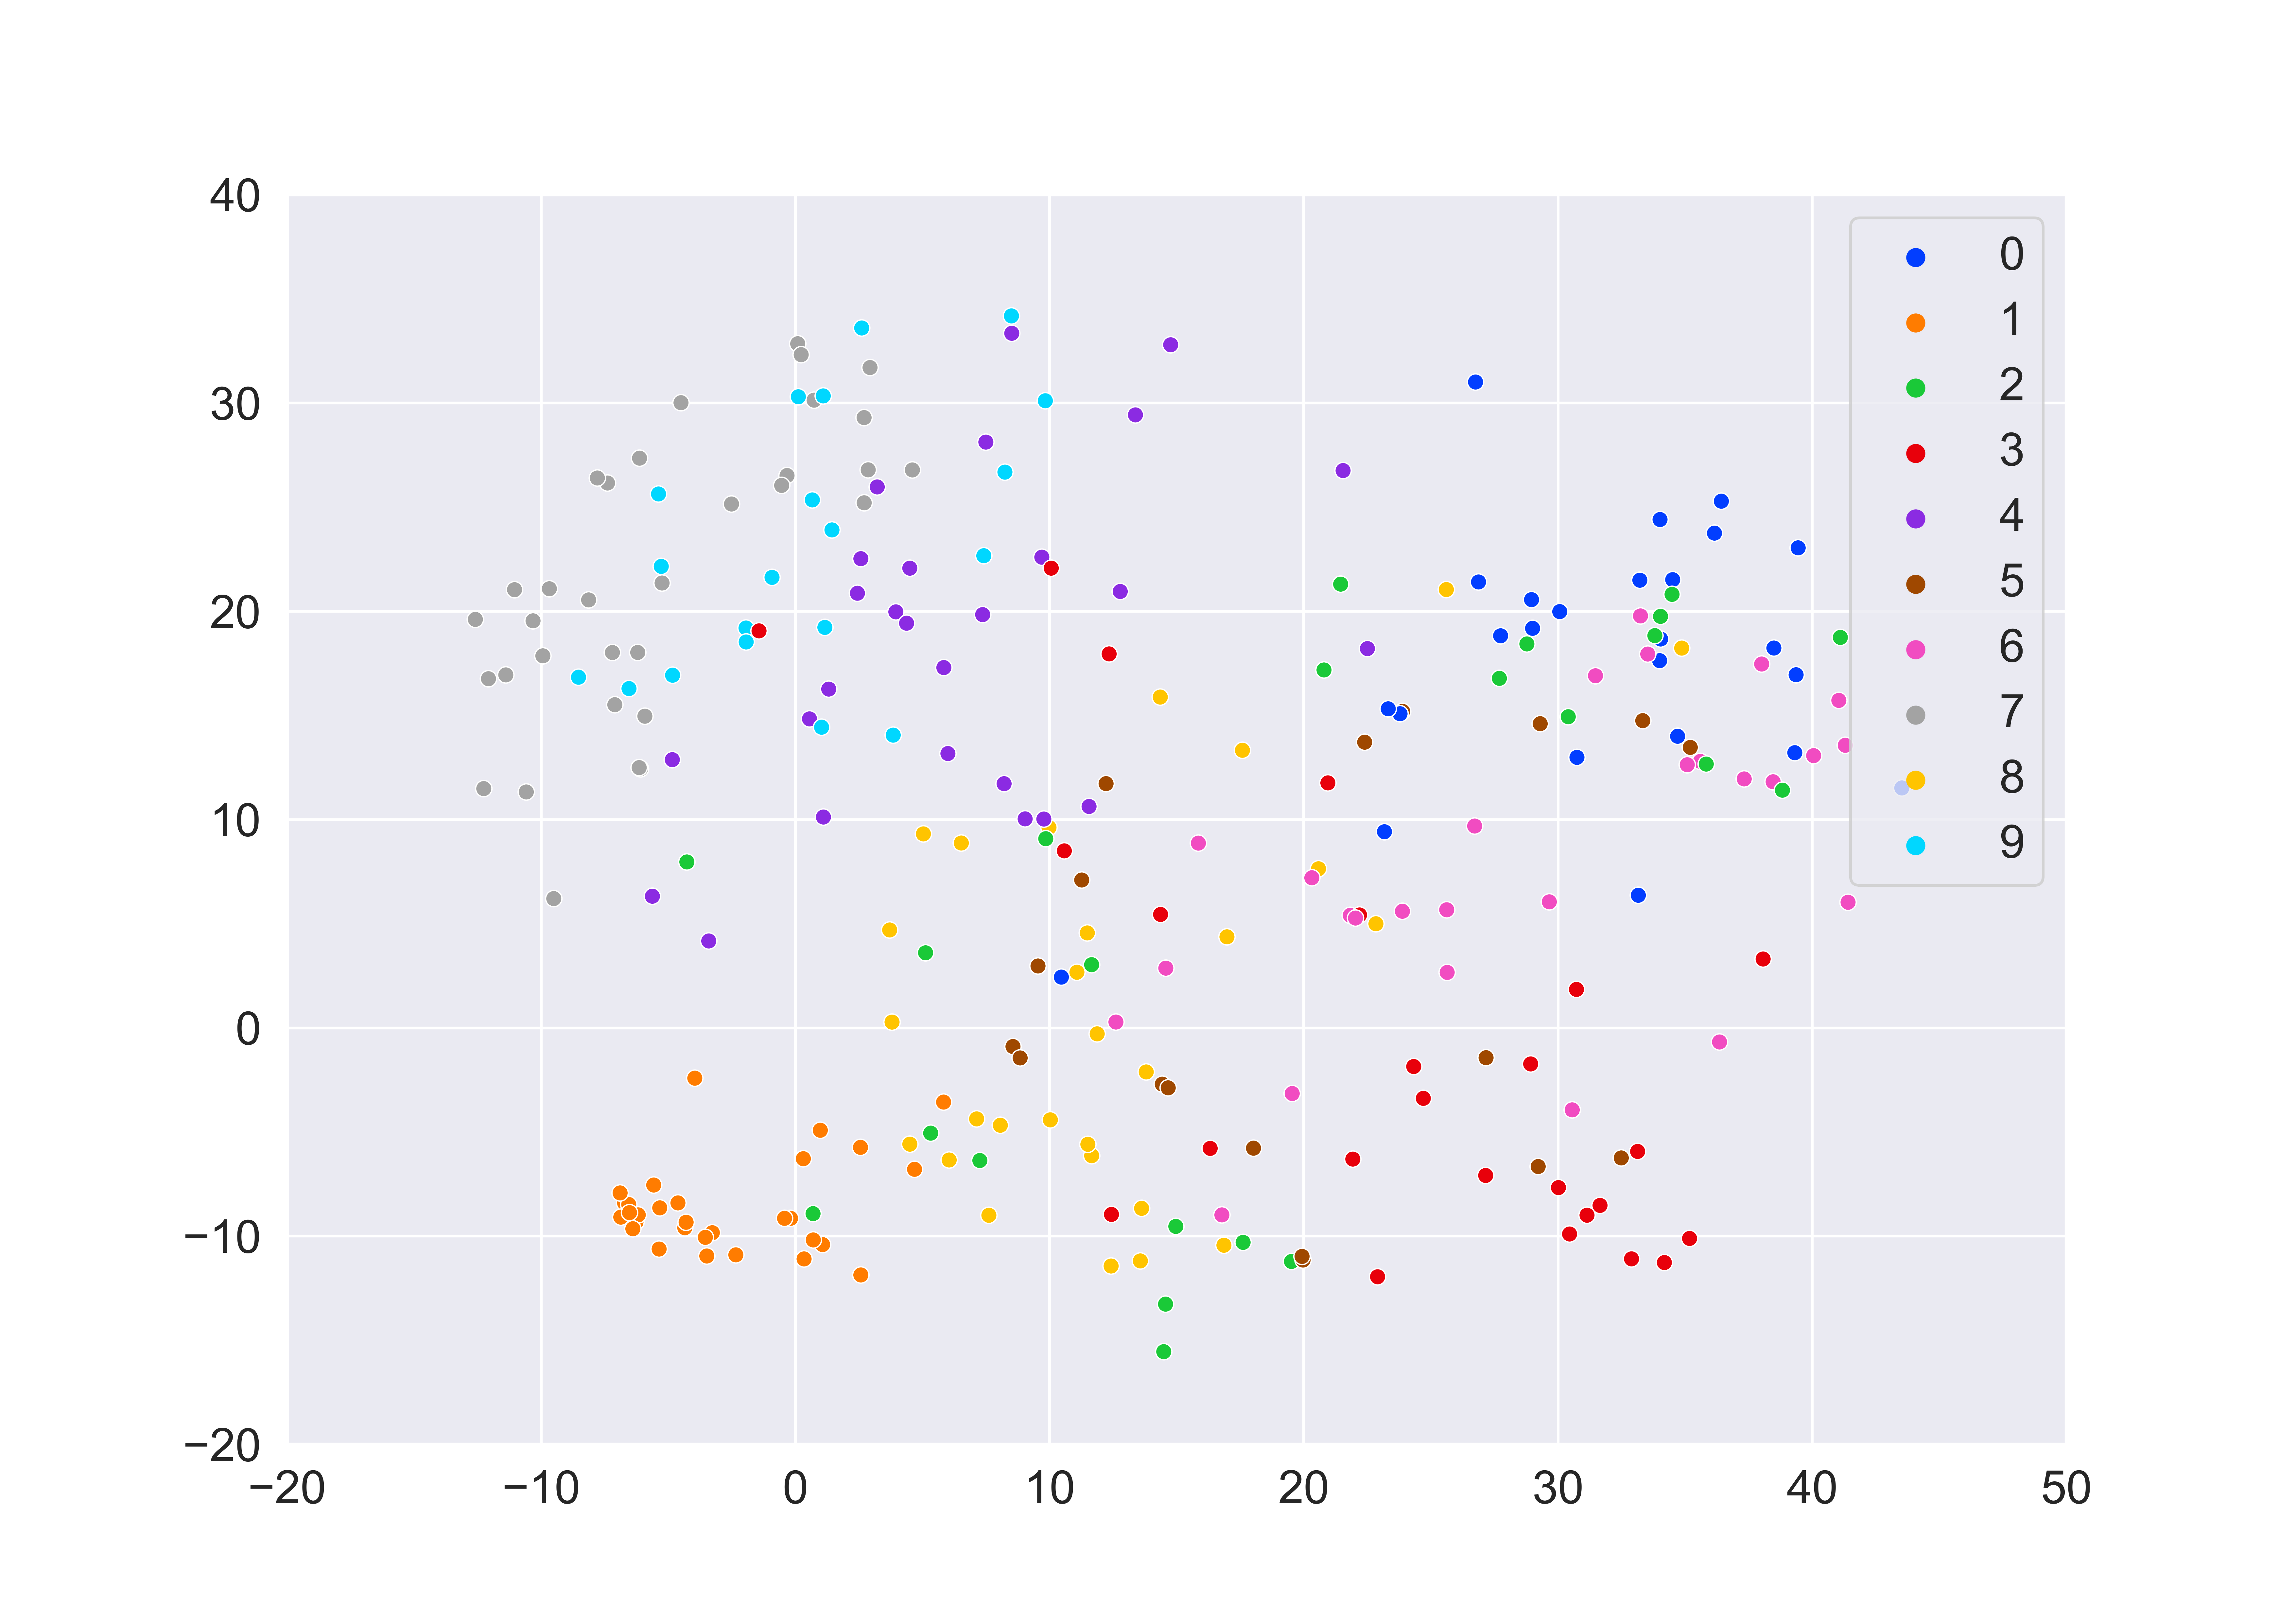
\includegraphics[width=0.32\linewidth]{../images/mnist_feature_map1_pca.png}
        % \caption{a}
        \label{fig:mnist_pca_1}
    \end{subfigure}
    % \hfill 
    \begin{subfigure}
        \centering
        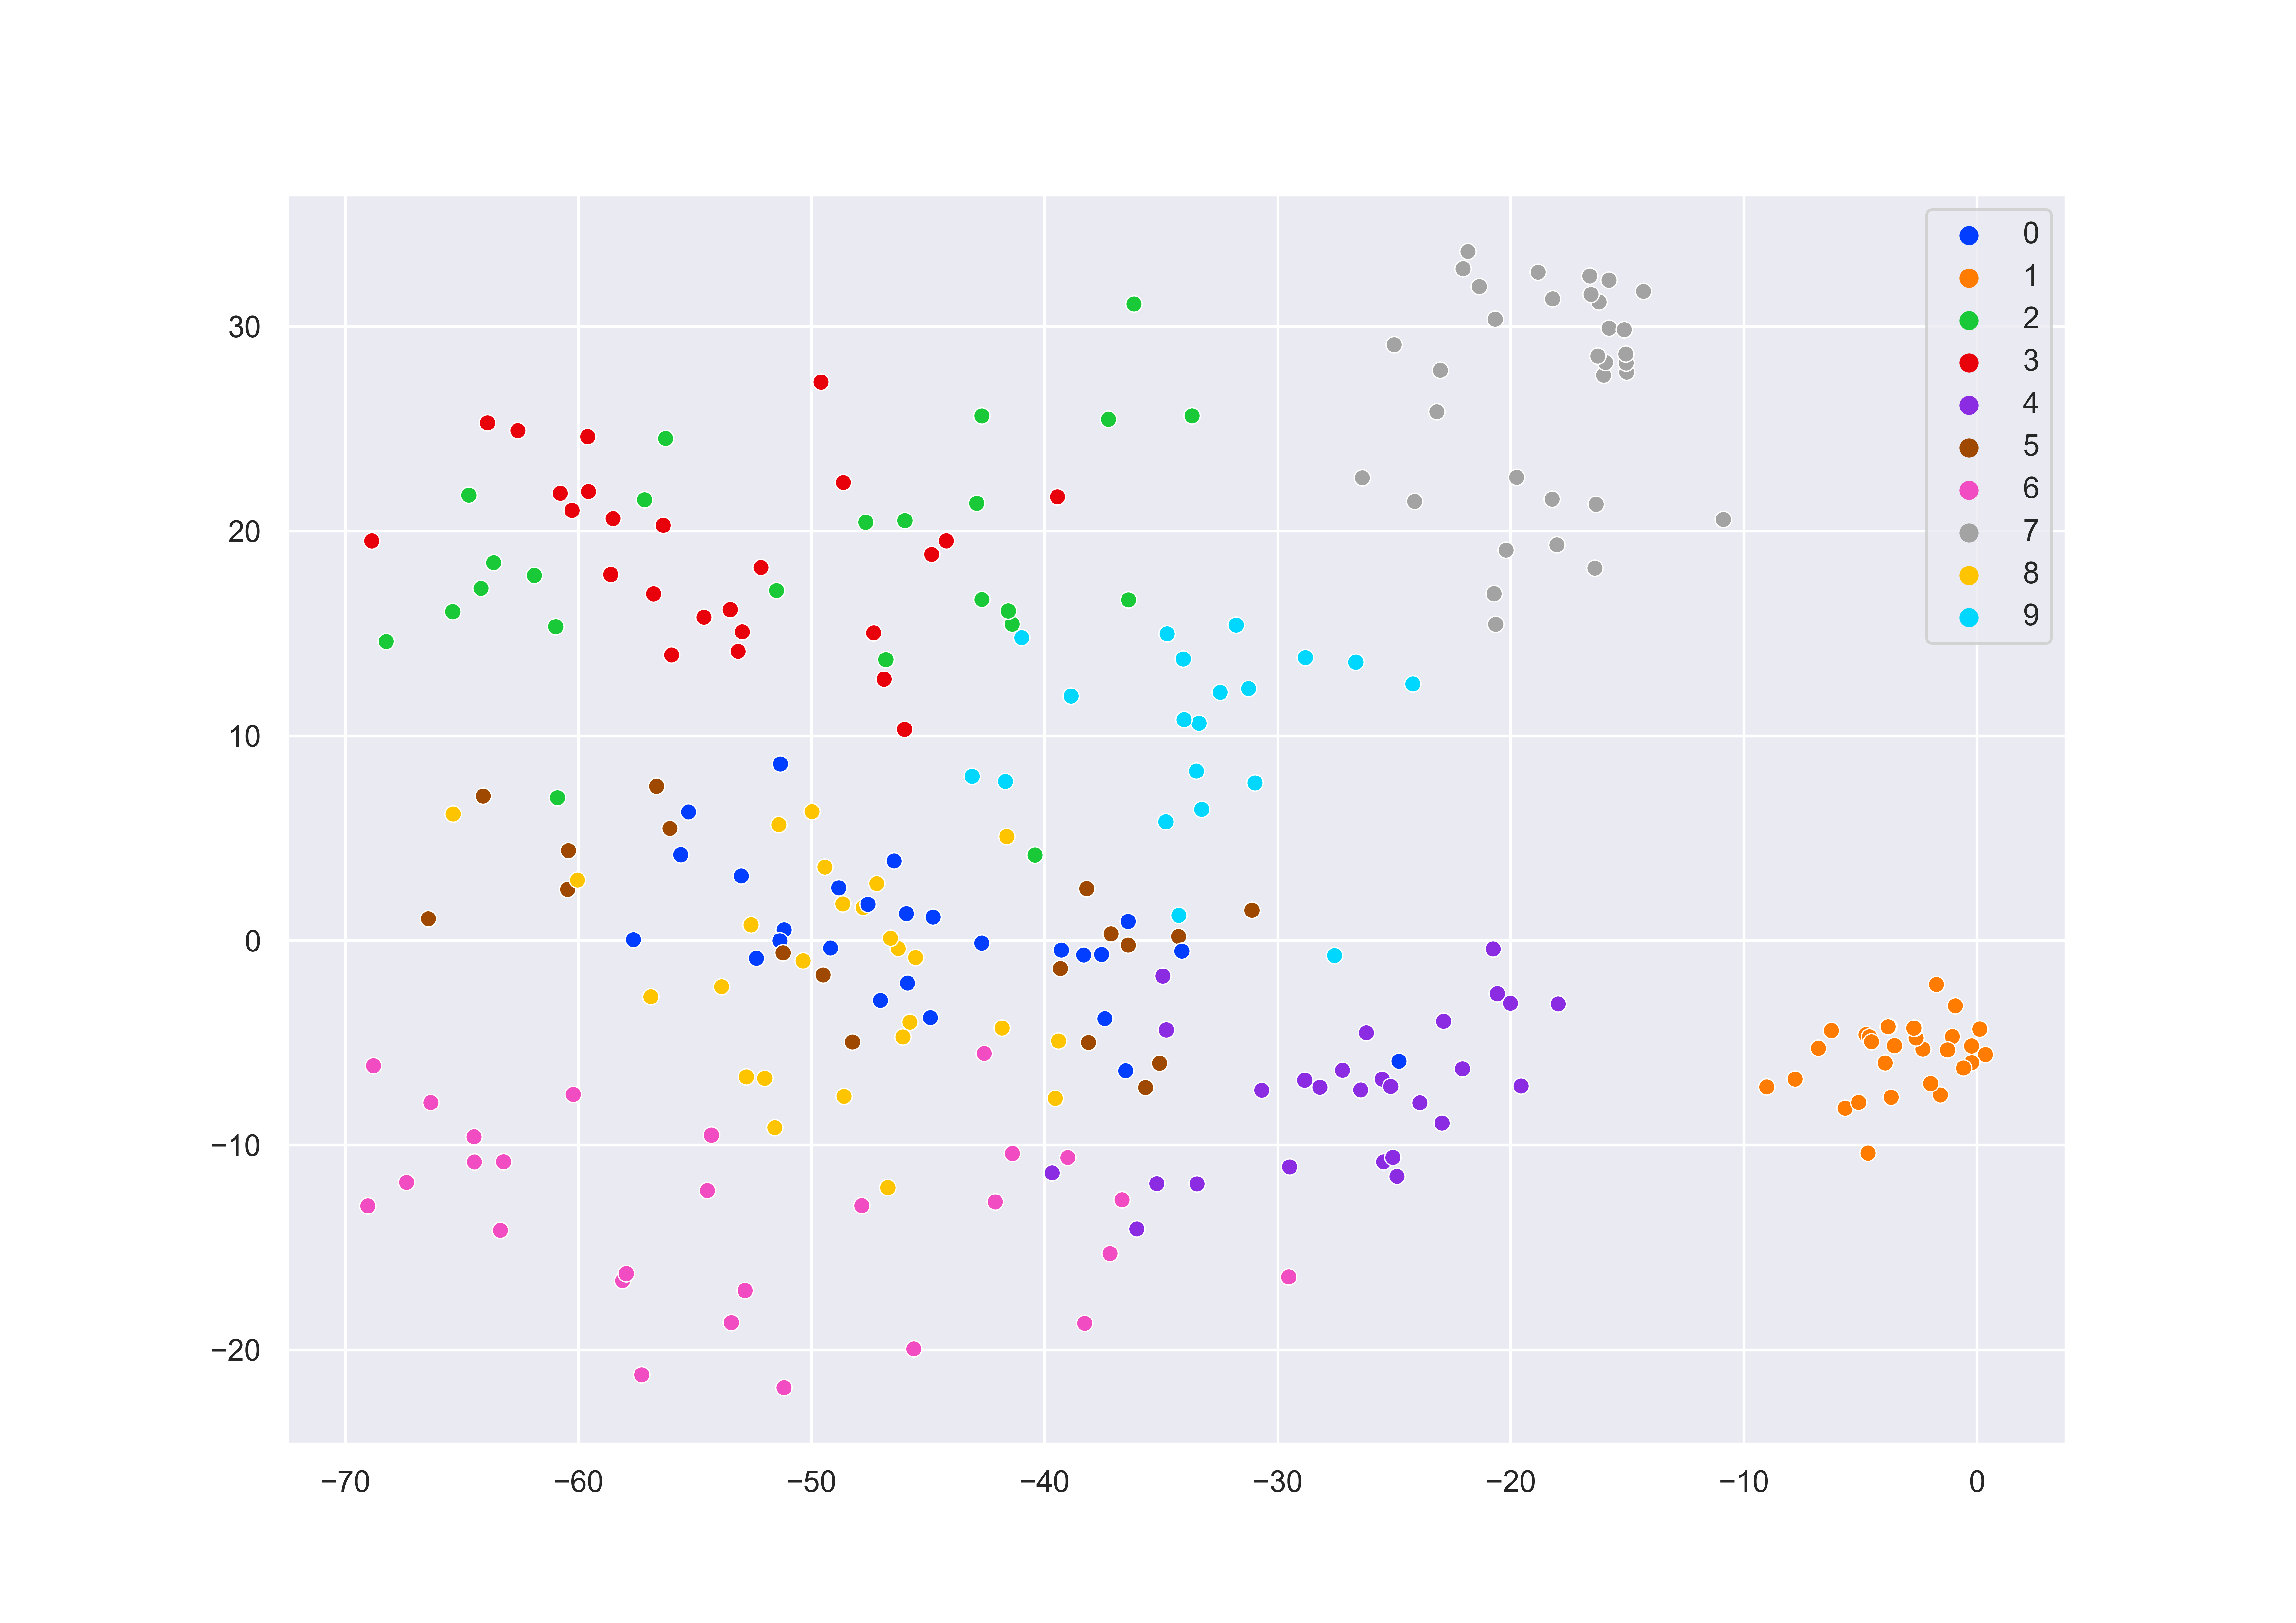
\includegraphics[width=0.32\linewidth]{../images/mnist_feature_map2_pca.png}
        % \caption{Absolute value of indivisual components of weight in ridge regression when setting $\lambda$ to 1.0.}
        \label{fig:mnist_pca_2}
    \end{subfigure}
    % \hfill 
    \begin{subfigure}
        \centering
        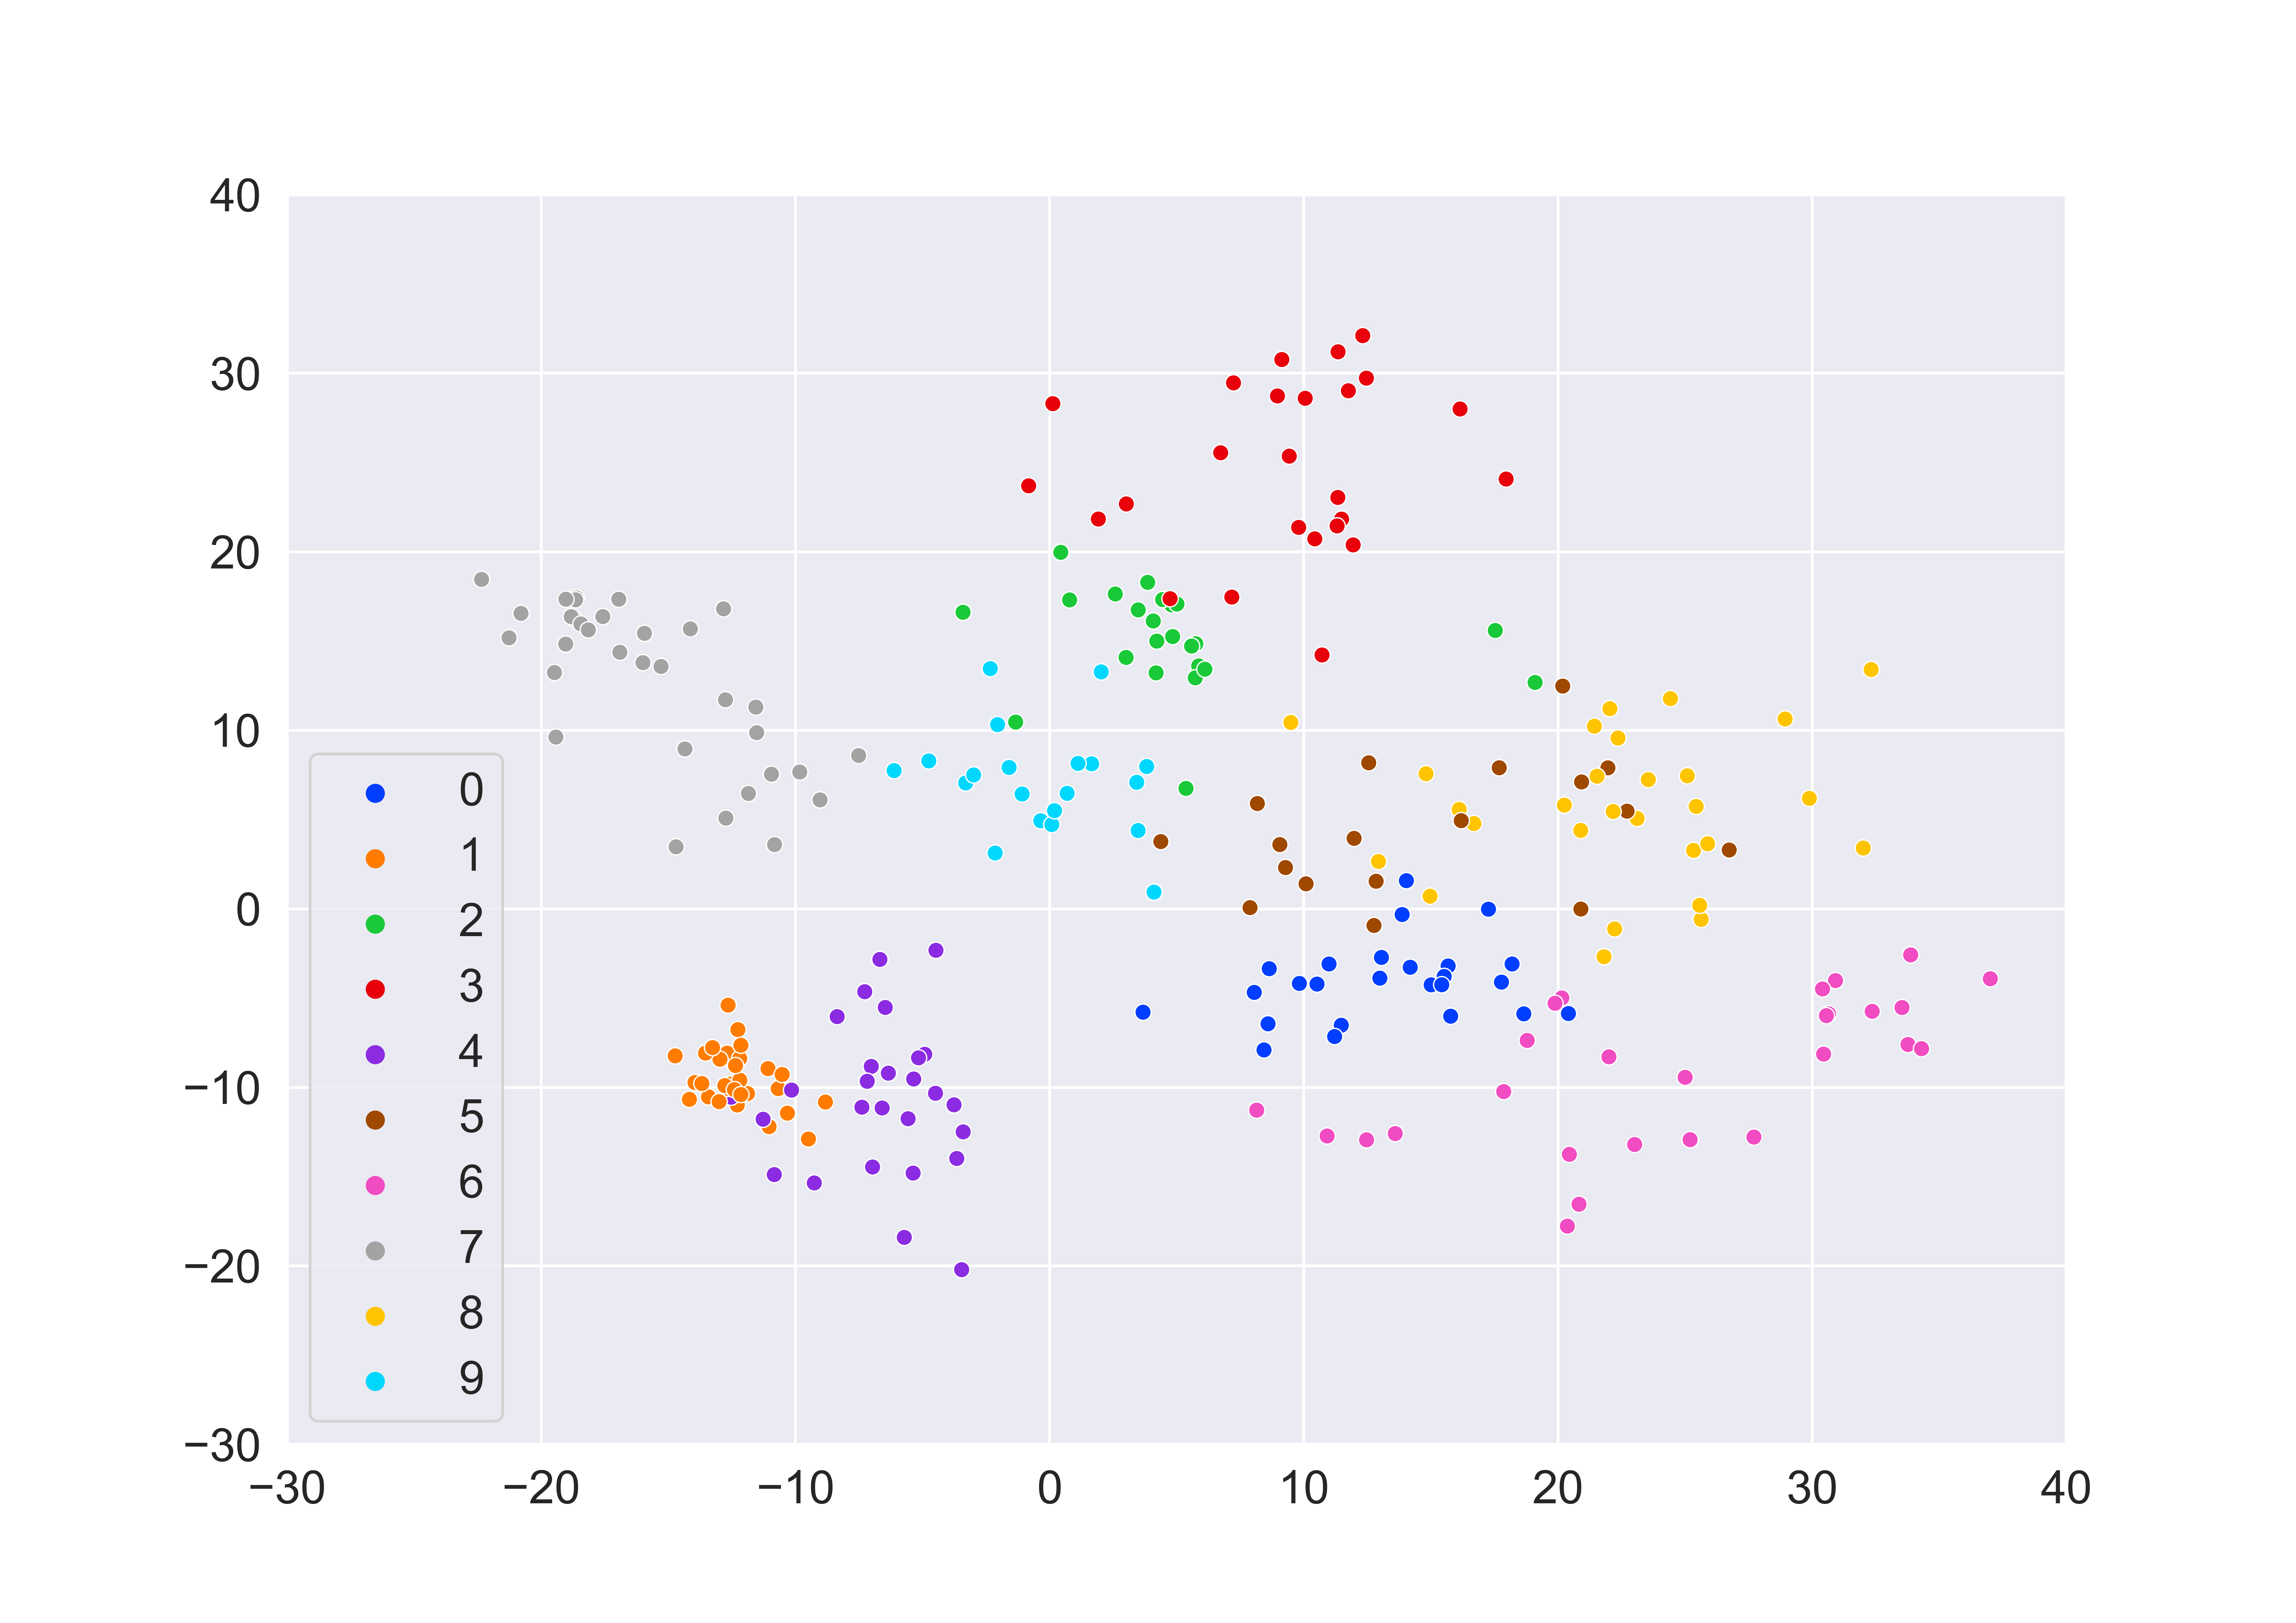
\includegraphics[width=0.32\linewidth]{../images/mnist_feature_map3_pca.png}
        % \caption{Absolute value of indivisual components of weight in ridge regression when setting $\lambda$ to 1.5.}
        \label{fig:mnist_pca_3}
    \end{subfigure}
    \caption{Visualization images of intermediate output tensors with PCA method. Left: Tensors after the first max pooling layer. Middle: Tensors after the second max pooling layer. Right: Tensors after the output linear layer.}
    \label{fig:mnist_pca}
\end{figure}

\begin{figure}[htbp]
    \centering
    \begin{subfigure}
        \centering
        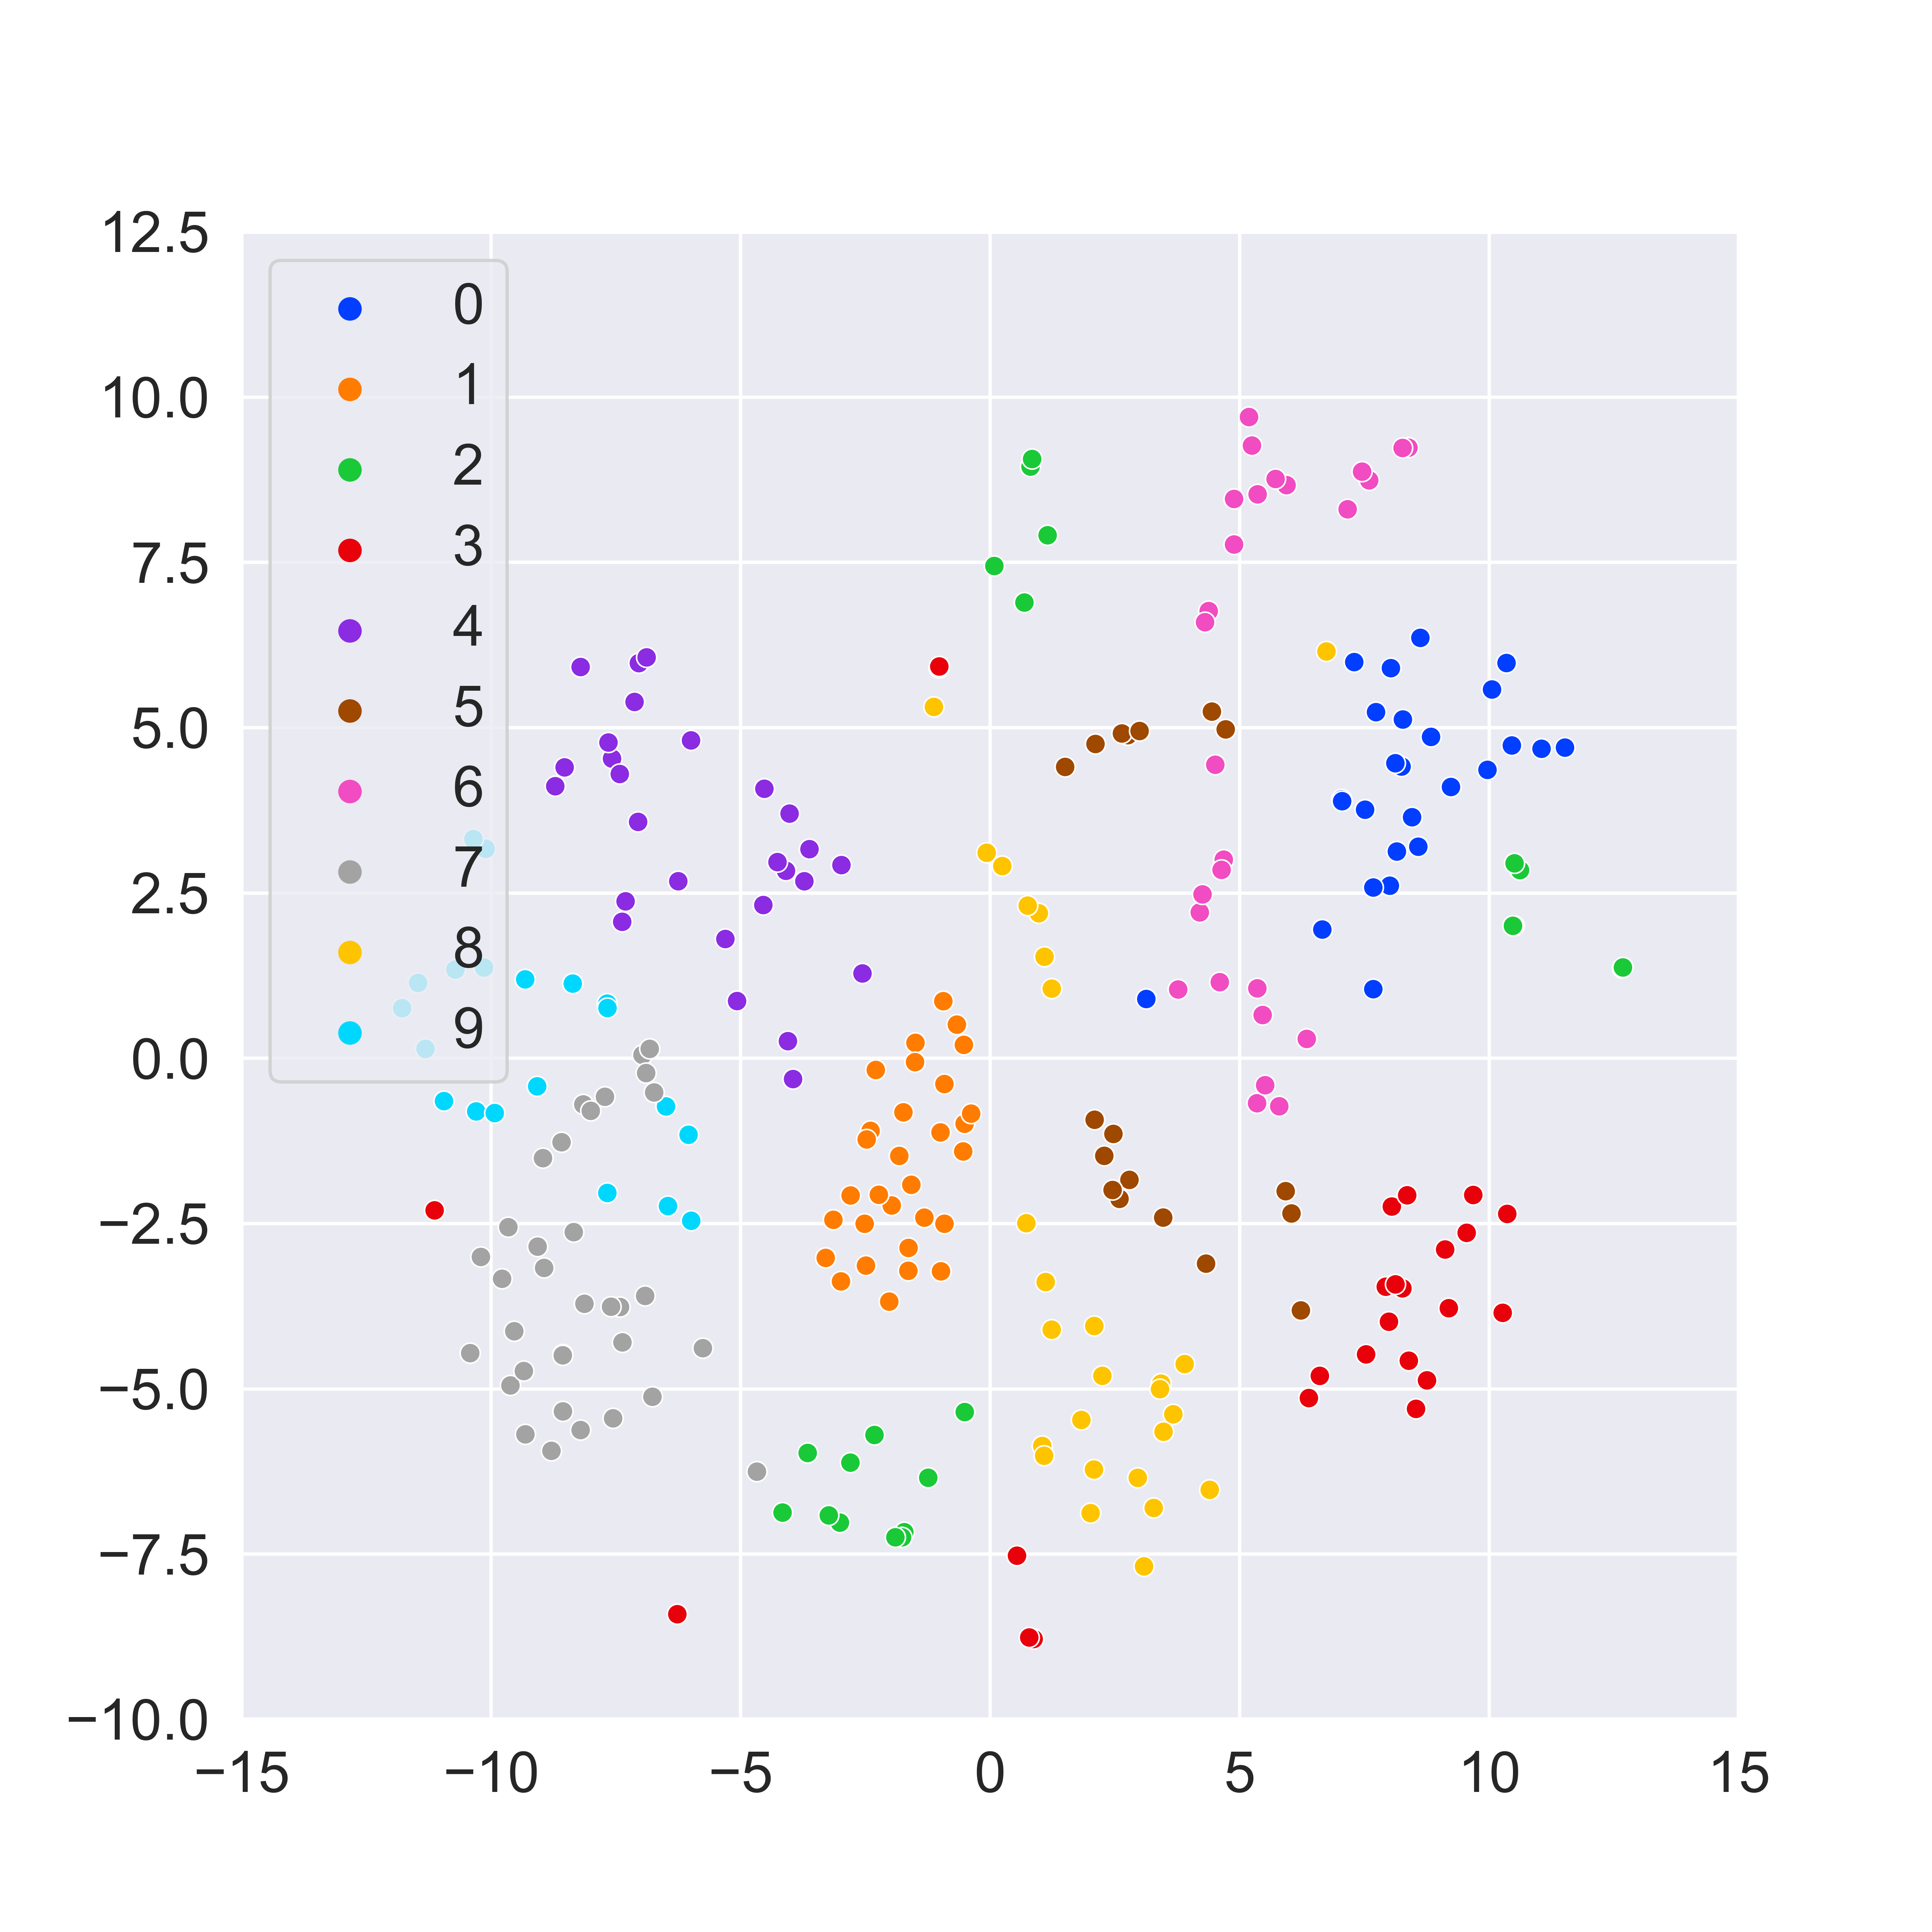
\includegraphics[width=0.32\linewidth]{../images/mnist_feature_map1_tsne.png}
        % \caption{a}
        \label{fig:mnist_tSNE_1}
    \end{subfigure}
    % \hfill 
    \begin{subfigure}
        \centering
        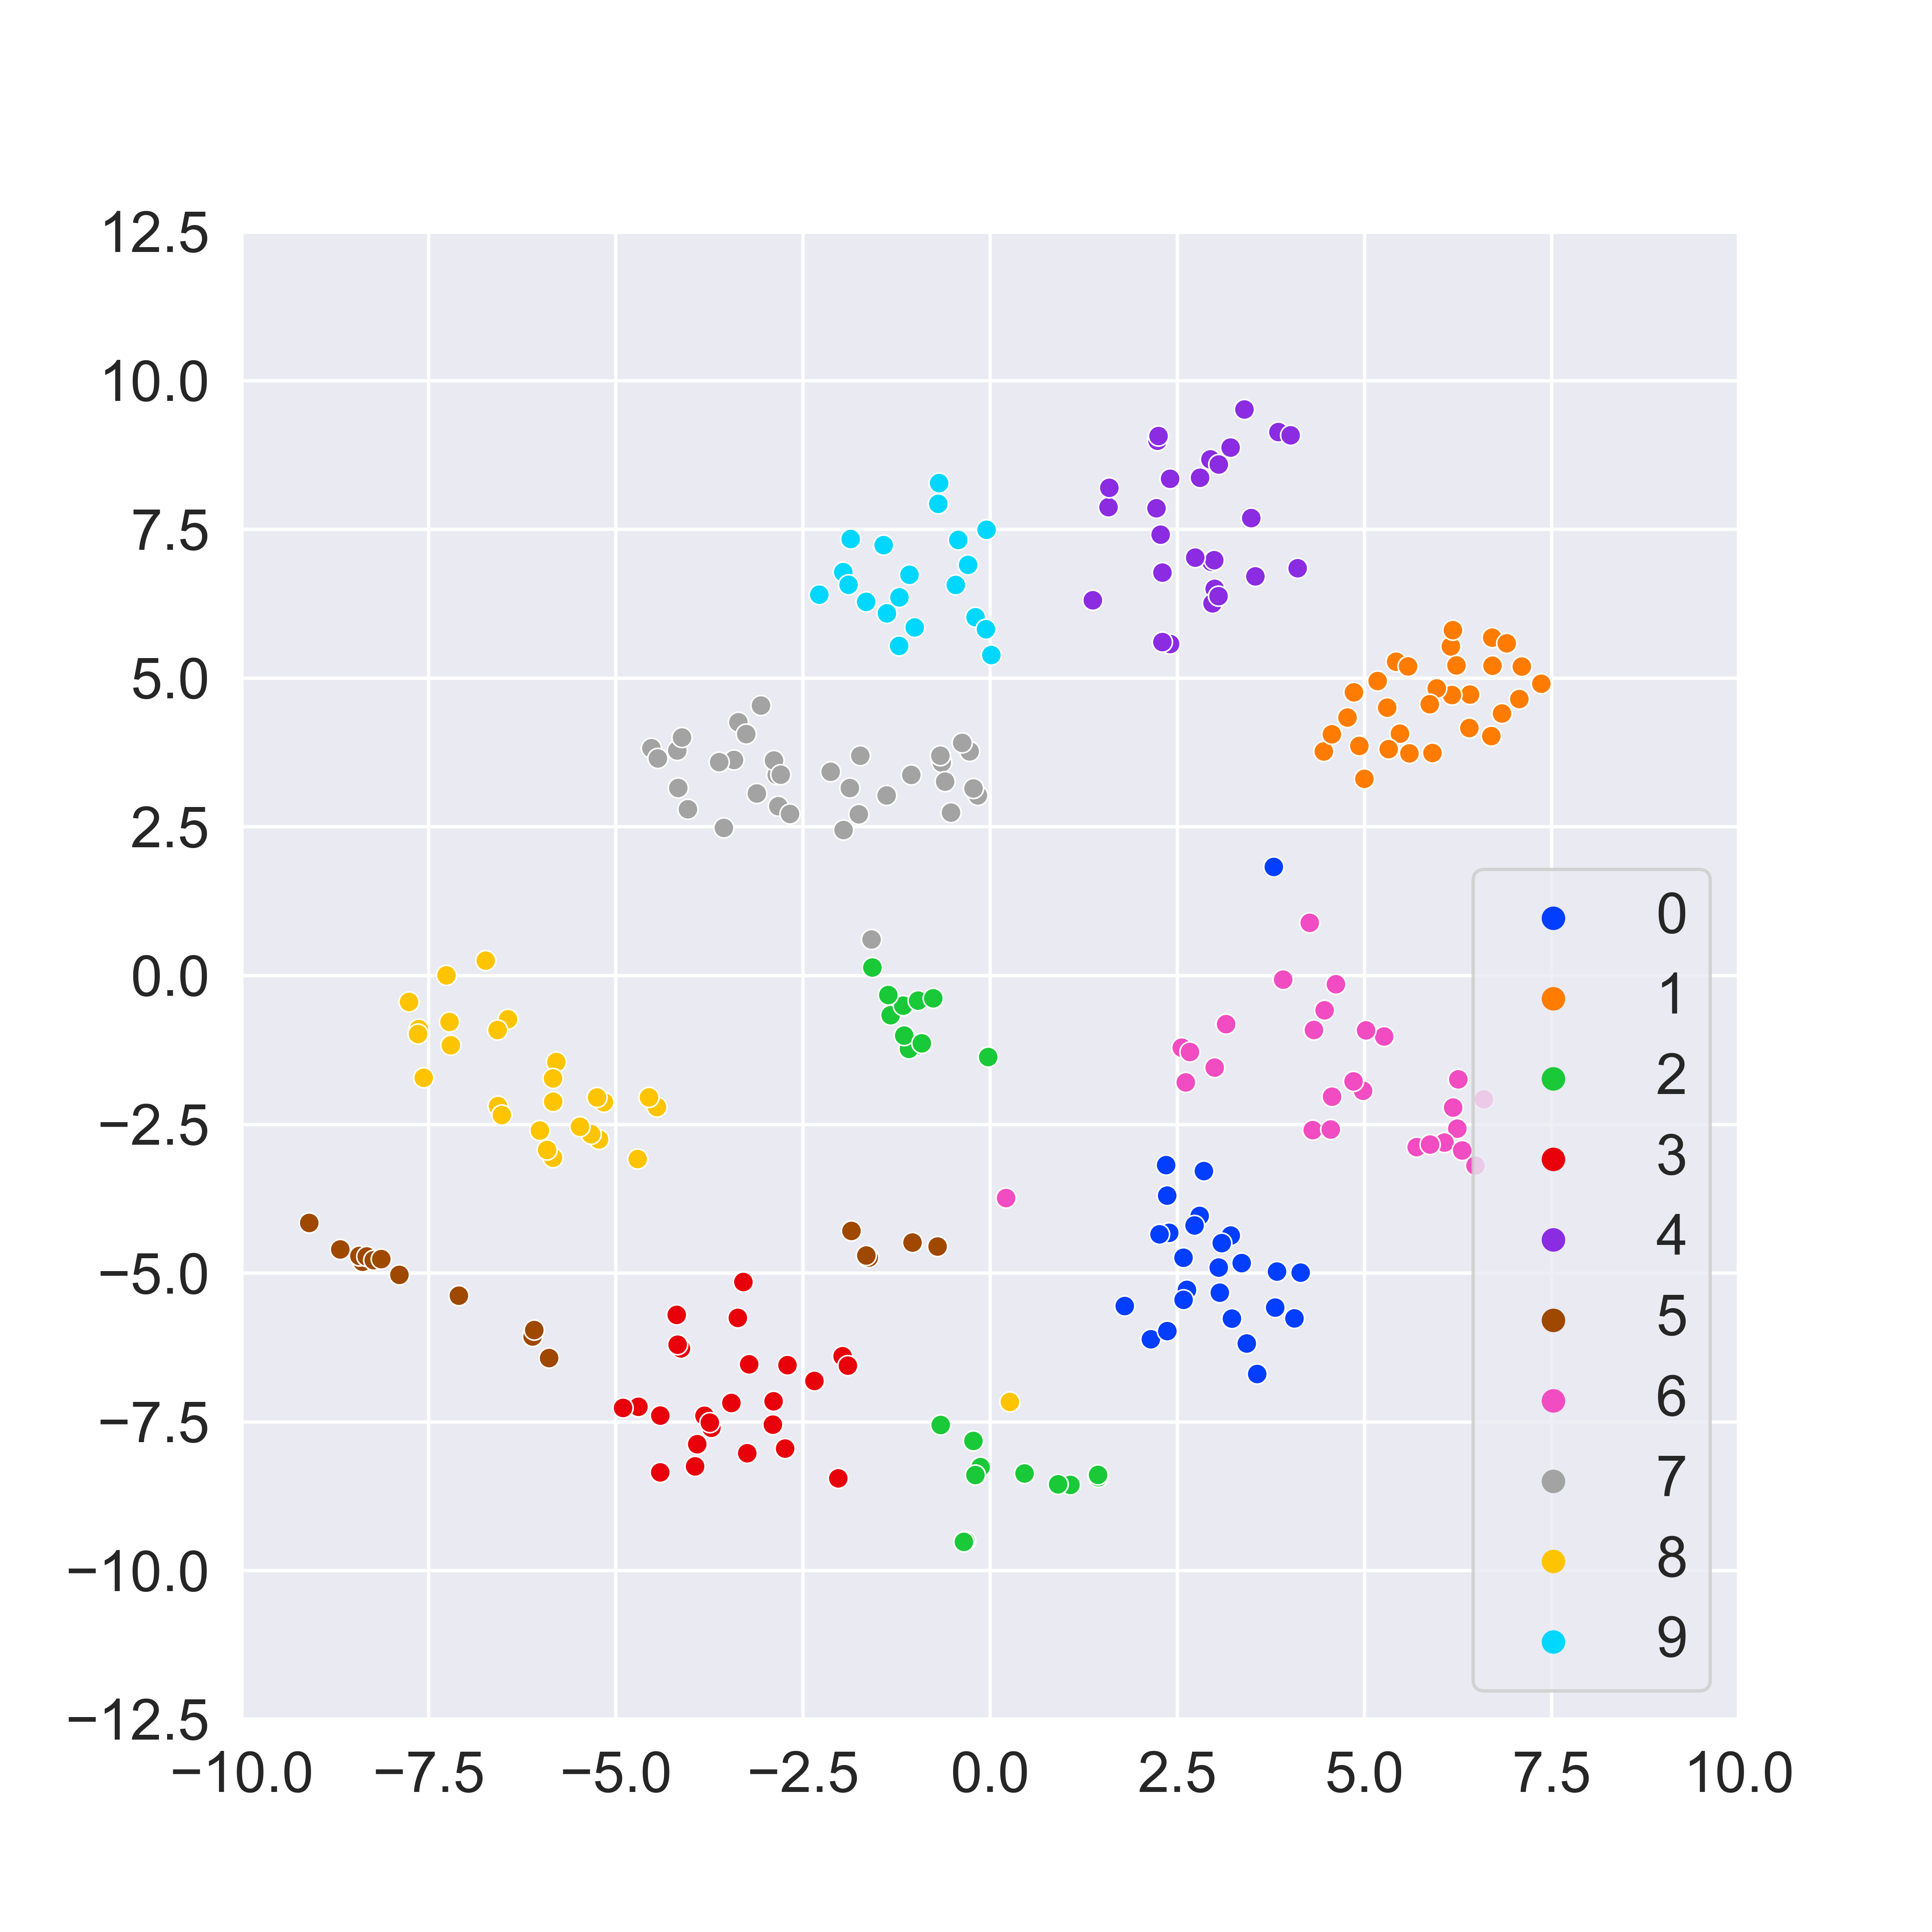
\includegraphics[width=0.32\linewidth]{../images/mnist_feature_map2_tsne.png}
        % \caption{Absolute value of indivisual components of weight in ridge regression when setting $\lambda$ to 1.0.}
        \label{fig:mnist_tSNE_2}
    \end{subfigure}
    % \hfill 
    \begin{subfigure}
        \centering
        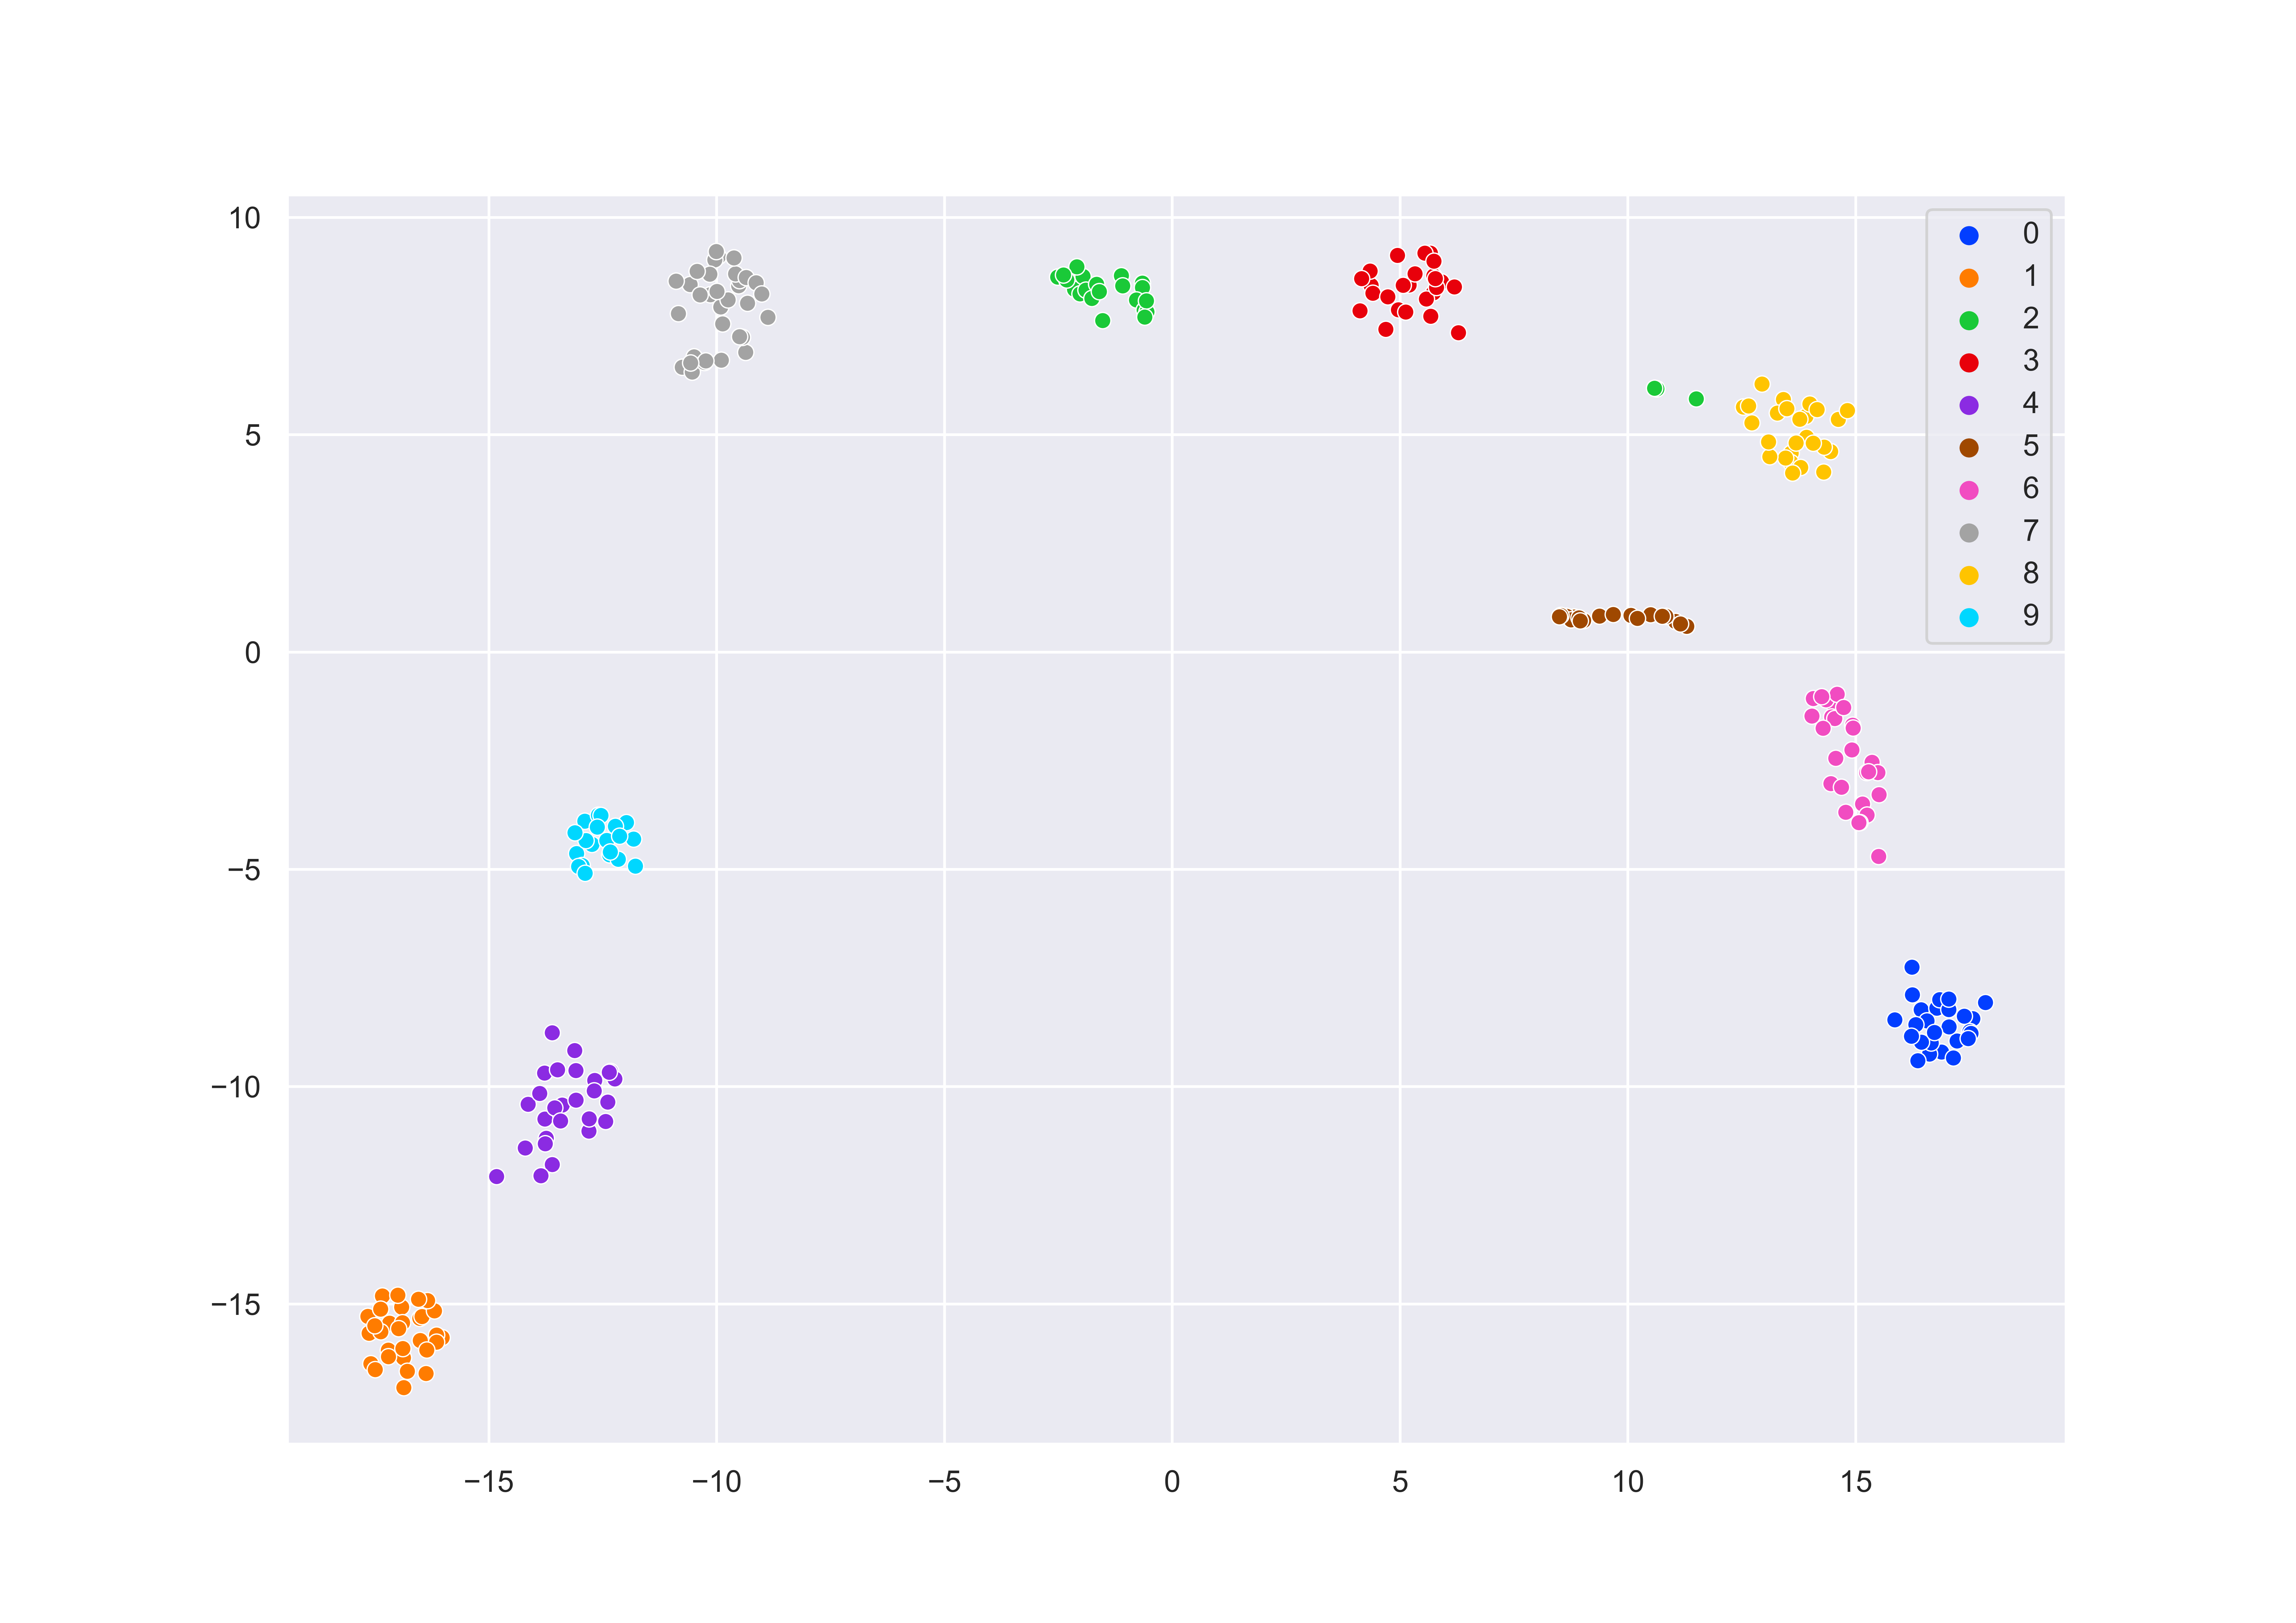
\includegraphics[width=0.32\linewidth]{../images/mnist_feature_map3_tsne.png}
        % \caption{Absolute value of indivisual components of weight in ridge regression when setting $\lambda$ to 1.5.}
        \label{fig:mnist_tSNE_3}
    \end{subfigure}
    \caption{Visualization images of intermediate output tensors with t-SNE method. Left: Tensors after the first max pooling layer. Middle: Tensors after the second max pooling layer. Right: Tensors after the output linear layer.}
    \label{fig:mnist_tsne}
\end{figure}
\section{Image Classification}

\subsection{Model \& Hyperparameters}
I design a 2-layer CNN models with an additional linear and softmax layer. The architecture can be interpreted in Fig.~\ref{fig:CNN_arch}. 
I set the batch size to 256 so as to maintain the high capability of batch normalization layer. 
The learning rate is set to 0.001 and the dropout rate is set to 0.1.
I train the whole model for 30 epochs and select the checkpoint with best binary cross entropy loss for evaluation on test set.

\subsection{Loss Function}
Because it is a classification task. I should have used cross entropy loss. 
But for training stability, I add an additional logarithm layer after the output softmax layer and use \verb|nn.LogSoftmax| instead of \verb|nn.Softmax| in pytorch.
So the loss function is simultaneously changed to negative log-liklihood loss.
\begin{equation}
    \label{eq:nllloss}
    \mathcal{L}=-\sum_{i}\sum_{k}y_k^*\cdot y_k
\end{equation}
where $k=1,2,\cdots, K$ and $K$ is the number of classes.

\subsection{Experiment Results}
The selected checkpoint can achieve $99.39\%$ accuracy in test set. The loss and accuracy change figures of self-designed CNN model are depicted in Fig.~\ref{fig:cnn_loss_acc}. It can be seen that the change is smooth, which proves that the hyperparameters are well-set and does not require more tuning steps.
\newline
\newline
\noindent 
Besides, I output the tensor after the first pooling layer, the tensor after the second pooling layer and the tensor after the output linear layer. 
And then I use PCA and t-SNE to respectively visualize them in order to see what my model has learned during training.
Their corresponding results are depicted in Fig.~\ref{fig:mnist_pca} and Fig.~\ref{fig:mnist_tsne}, respectively.
It can be seen that the first tensor cannot distinguish well each images but after the second CNN layer, my model has learned to distinguish each image with high accuracy.
The corresponding PCA code is presented below and the t-SNE code is pasted at the end of the report. 
I follow the handout of Prof. Zhang to implement it by myself.
My implemented PCA method does not use eigen-decomposition based method because it costs a lot. 
Instead, I use SVD to extract main components which can also represent the feature of original data. 
The code for SVD is shown below and the main structure of code of t-SNE is shown in Sec.~\ref{code:tsne}
\begin{lstlisting}
class MyPCA:
    def __init__(self, n_components: int = 2) -> None:
        self.n = n_components
    
    def fit(self, X: np.ndarray):
        n_samples, n_features = X.shape
        assert n_features >= self.n, "Main components must be less than or equal to total feature numbers"
        mean_val = X.mean(0, keepdims=True)
        X = X - mean_val
        U, sigma, VT = np.linalg.svd(X, False)
        self.P = U[:, :self.n]
        max_abs_cols = np.argmax(np.abs(U), axis=0)
        signs = np.sign(U[max_abs_cols, range(U.shape[1])])
        U *= signs
        VT *= signs[:, np.newaxis]
        self.P = VT[:self.n]

        return self
    
    def transform(self, X):
        return X @ self.P.T
\end{lstlisting}

\section{Image Generation}
\begin{figure}[htbp]
    \centering
    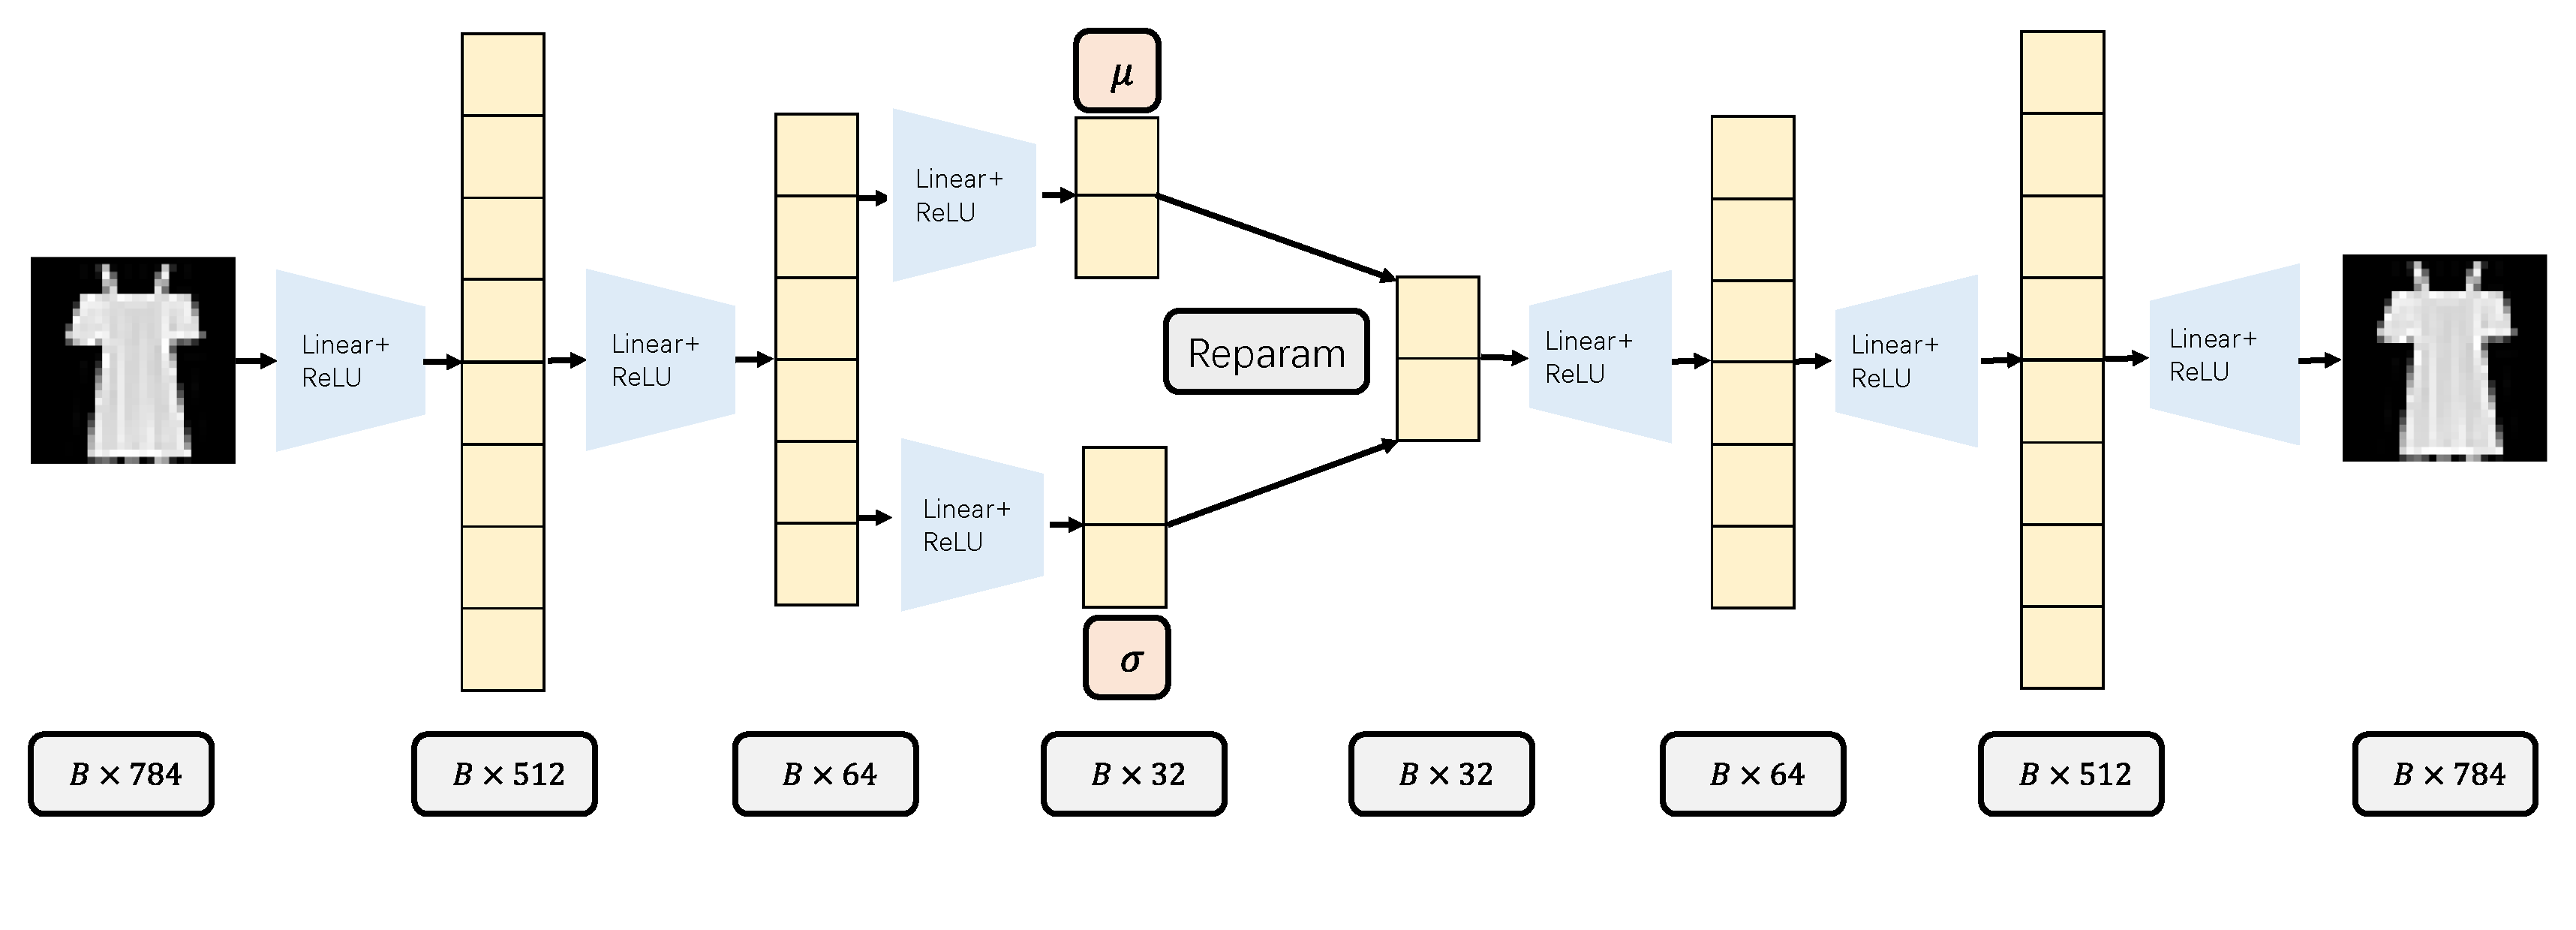
\includegraphics[width=0.95\textwidth]{vae_model.pdf}
    \caption{VAE model framework. }
    \label{fig:vae_model}
\end{figure}
\subsection{Model \& Hyperparameters}
Two different datasets are provided and what I have chosen is FashionMnist dataset, which contains 70000 images with 10 different classes. 
I use 60000 images as the training set and train my VAE model on it.
For evaluation, I randomly initialize two Gaussian noise and use the trained decoder and specified $\alpha$ value to separately output the generated images.
\newline
\newline
\noindent 
I ran my VAE model for 50 epochs.
The batch size is set to 256 for better generalization.
The learning rate is again set to $0.001$.
The detailed model is presented in Fig.~\ref{fig:vae_model}.
In encoder, I use two linear models and respectively learn the expectation and variance of latent normal distribution.
Because outputs of neural networks are not controllable, I choose to learn the logarithm value of variance instead of directly learning variance.
To obtain the variance, the only thing to do is to execute exponential operation, which is convenient and fast.
To obtain the encoded Gaussian noise, the reparameterization is required and shown on below:
\begin{equation}
    \boldsymbol{p} = \mu + \mathrm{exp}(\log(\sigma ^2) / 2)\cdot \boldsymbol{q}
\end{equation}
where $\boldsymbol{q}$ is a Gaussian noise and $\mu$ is the predicted expectation and $\sigma$ is the predicted standard deviation. 
I omit two implementation steps in input stage and output state, where I flatten the image to a 1D array.

\begin{figure}[htbp]
    \centering
    \begin{subfigure}
        \centering
        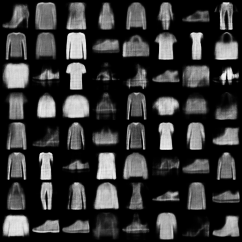
\includegraphics[width=0.45\linewidth]{../images/vae-image1.png}
        % \caption{a}
        \label{fig:vae_image1}
    \end{subfigure}
    % \hfill 
    \begin{subfigure}
        \centering
        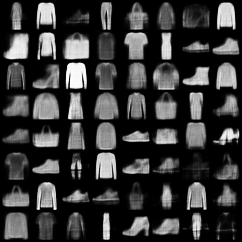
\includegraphics[width=0.45\linewidth]{../images/vae-image2.png}
        % \caption{Absolute value of indivisual components of weight in ridge regression when setting $\lambda$ to 1.0.}
        \label{fig:vae_image2}
    \end{subfigure}
    
    \caption{Two groups of images generated by two batches of random Gaussian noise.}
    \label{fig:vae_original_image}
\end{figure}

\begin{figure}[htbp]
    \centering
    \begin{subfigure}
        \centering
        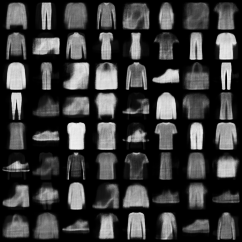
\includegraphics[width=0.32\linewidth]{../images/vae-0.10-merge.png}
        % \caption{a}
        \label{fig:vae_0.1}
    \end{subfigure}
    % \hfill 
    \begin{subfigure}
        \centering
        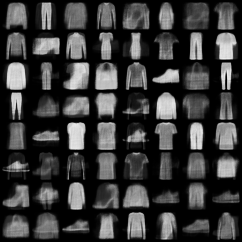
\includegraphics[width=0.32\linewidth]{../images/vae-0.20-merge.png}
        % \caption{Absolute value of indivisual components of weight in ridge regression when setting $\lambda$ to 1.0.}
        \label{fig:vae_0.2}
    \end{subfigure}
    \begin{subfigure}
        \centering
        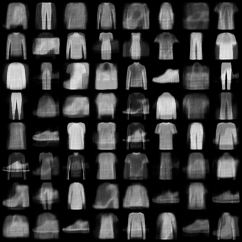
\includegraphics[width=0.32\linewidth]{../images/vae-0.30-merge.png}
        % \caption{Absolute value of indivisual components of weight in ridge regression when setting $\lambda$ to 1.0.}
        \label{fig:vae_0.3}
    \end{subfigure}
    \begin{subfigure}
        \centering
        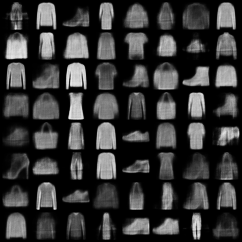
\includegraphics[width=0.32\linewidth]{../images/vae-0.40-merge.png}
        % \caption{Absolute value of indivisual components of weight in ridge regression when setting $\lambda$ to 1.0.}
        \label{fig:vae_0.4}
    \end{subfigure}
    \begin{subfigure}
        \centering
        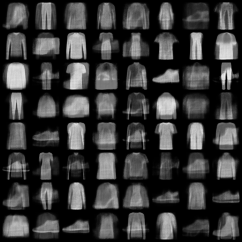
\includegraphics[width=0.32\linewidth]{../images/vae-0.50-merge.png}
        % \caption{Absolute value of indivisual components of weight in ridge regression when setting $\lambda$ to 1.0.}
        \label{fig:vae_0.5}
    \end{subfigure}
    \begin{subfigure}
        \centering
        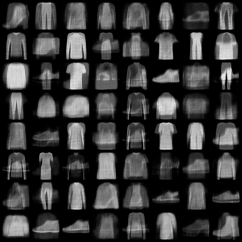
\includegraphics[width=0.32\linewidth]{../images/vae-0.60-merge.png}
        % \caption{Absolute value of indivisual components of weight in ridge regression when setting $\lambda$ to 1.0.}
        \label{fig:vae_0.6}
    \end{subfigure}
    \begin{subfigure}
        \centering
        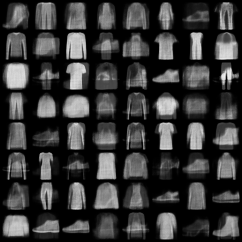
\includegraphics[width=0.32\linewidth]{../images/vae-0.70-merge.png}
        % \caption{Absolute value of indivisual components of weight in ridge regression when setting $\lambda$ to 1.0.}
        \label{fig:vae_0.7}
    \end{subfigure}
    \begin{subfigure}
        \centering
        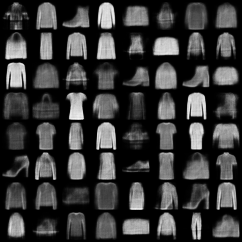
\includegraphics[width=0.32\linewidth]{../images/vae-0.80-merge.png}
        % \caption{Absolute value of indivisual components of weight in ridge regression when setting $\lambda$ to 1.0.}
        \label{fig:vae_0.8}
    \end{subfigure}
    \begin{subfigure}
        \centering
        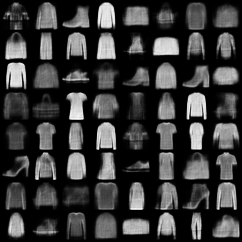
\includegraphics[width=0.32\linewidth]{../images/vae-0.90-merge.png}
        % \caption{Absolute value of indivisual components of weight in ridge regression when setting $\lambda$ to 1.0.}
        \label{fig:vae_0.9}
    \end{subfigure}
    
    \caption{These nine images represent different interpolation values $\alpha$. $\alpha$ values change from 0.1 to 0.9 from left top to right down.}
    \label{fig:vae_samples}
\end{figure}
\subsection{Experiment Result}
I first present two images generated from two random Gaussian noise in Fig.~\ref{fig:vae_original_image}. 
I display 64 different small images generated from a batch for each whole image.
For these two Gaussian noise $\boldsymbol{p}$ and $\boldsymbol{q}$ and use different $\alpha$ values to produce a new image as such:
\begin{align*}
    \mathbf{X}&=\texttt{VAE}(\boldsymbol{p}) \\
    \mathbf{Y}&=\texttt{VAE}(\boldsymbol{q}) \\
    \mathbf{Z}&=\texttt{VAE}(\alpha \boldsymbol{p}+(1-\alpha)\boldsymbol{q})
\end{align*}
where $\mathbf{X,Y,Z}$ represent the generated images and several different examples of $\mathbf{X}$ and $\mathbf{Y}$ are shown in Fig.~\ref{fig:vae_original_image}. 
These nine images represent how a image is transferred from one type of object to another type with different interpolation factors.
Let's look at the first images located at the first row and fourth column in two images in Fig.~\ref{fig:vae_original_image}, which are a T-shirt and a pair of pants, respectively.
Now the $\alpha$ changes from 0.1 to 0.9, which means that the image will transfer from a pair of pants to a T-shirt gradually.
And the images in Fig.~\ref{fig:vae_samples} verify the theoretical results. 
The VAE model implemented by myself can to some extent realize variational image generation.

\subsection{Discussion}
A random Gaussian noise can represent a specific property that the model has learned. But the images generated from VAE may vary according to different noise, which shows the strong variability of VAE models compared to GAN-related models. 
Although GAN models can generate images extremely similar to the original images, they lose the ability to generate diverse images, which is the strength of VAE models.

\section{Sentiment Analysis}
\begin{figure}
    \centering
    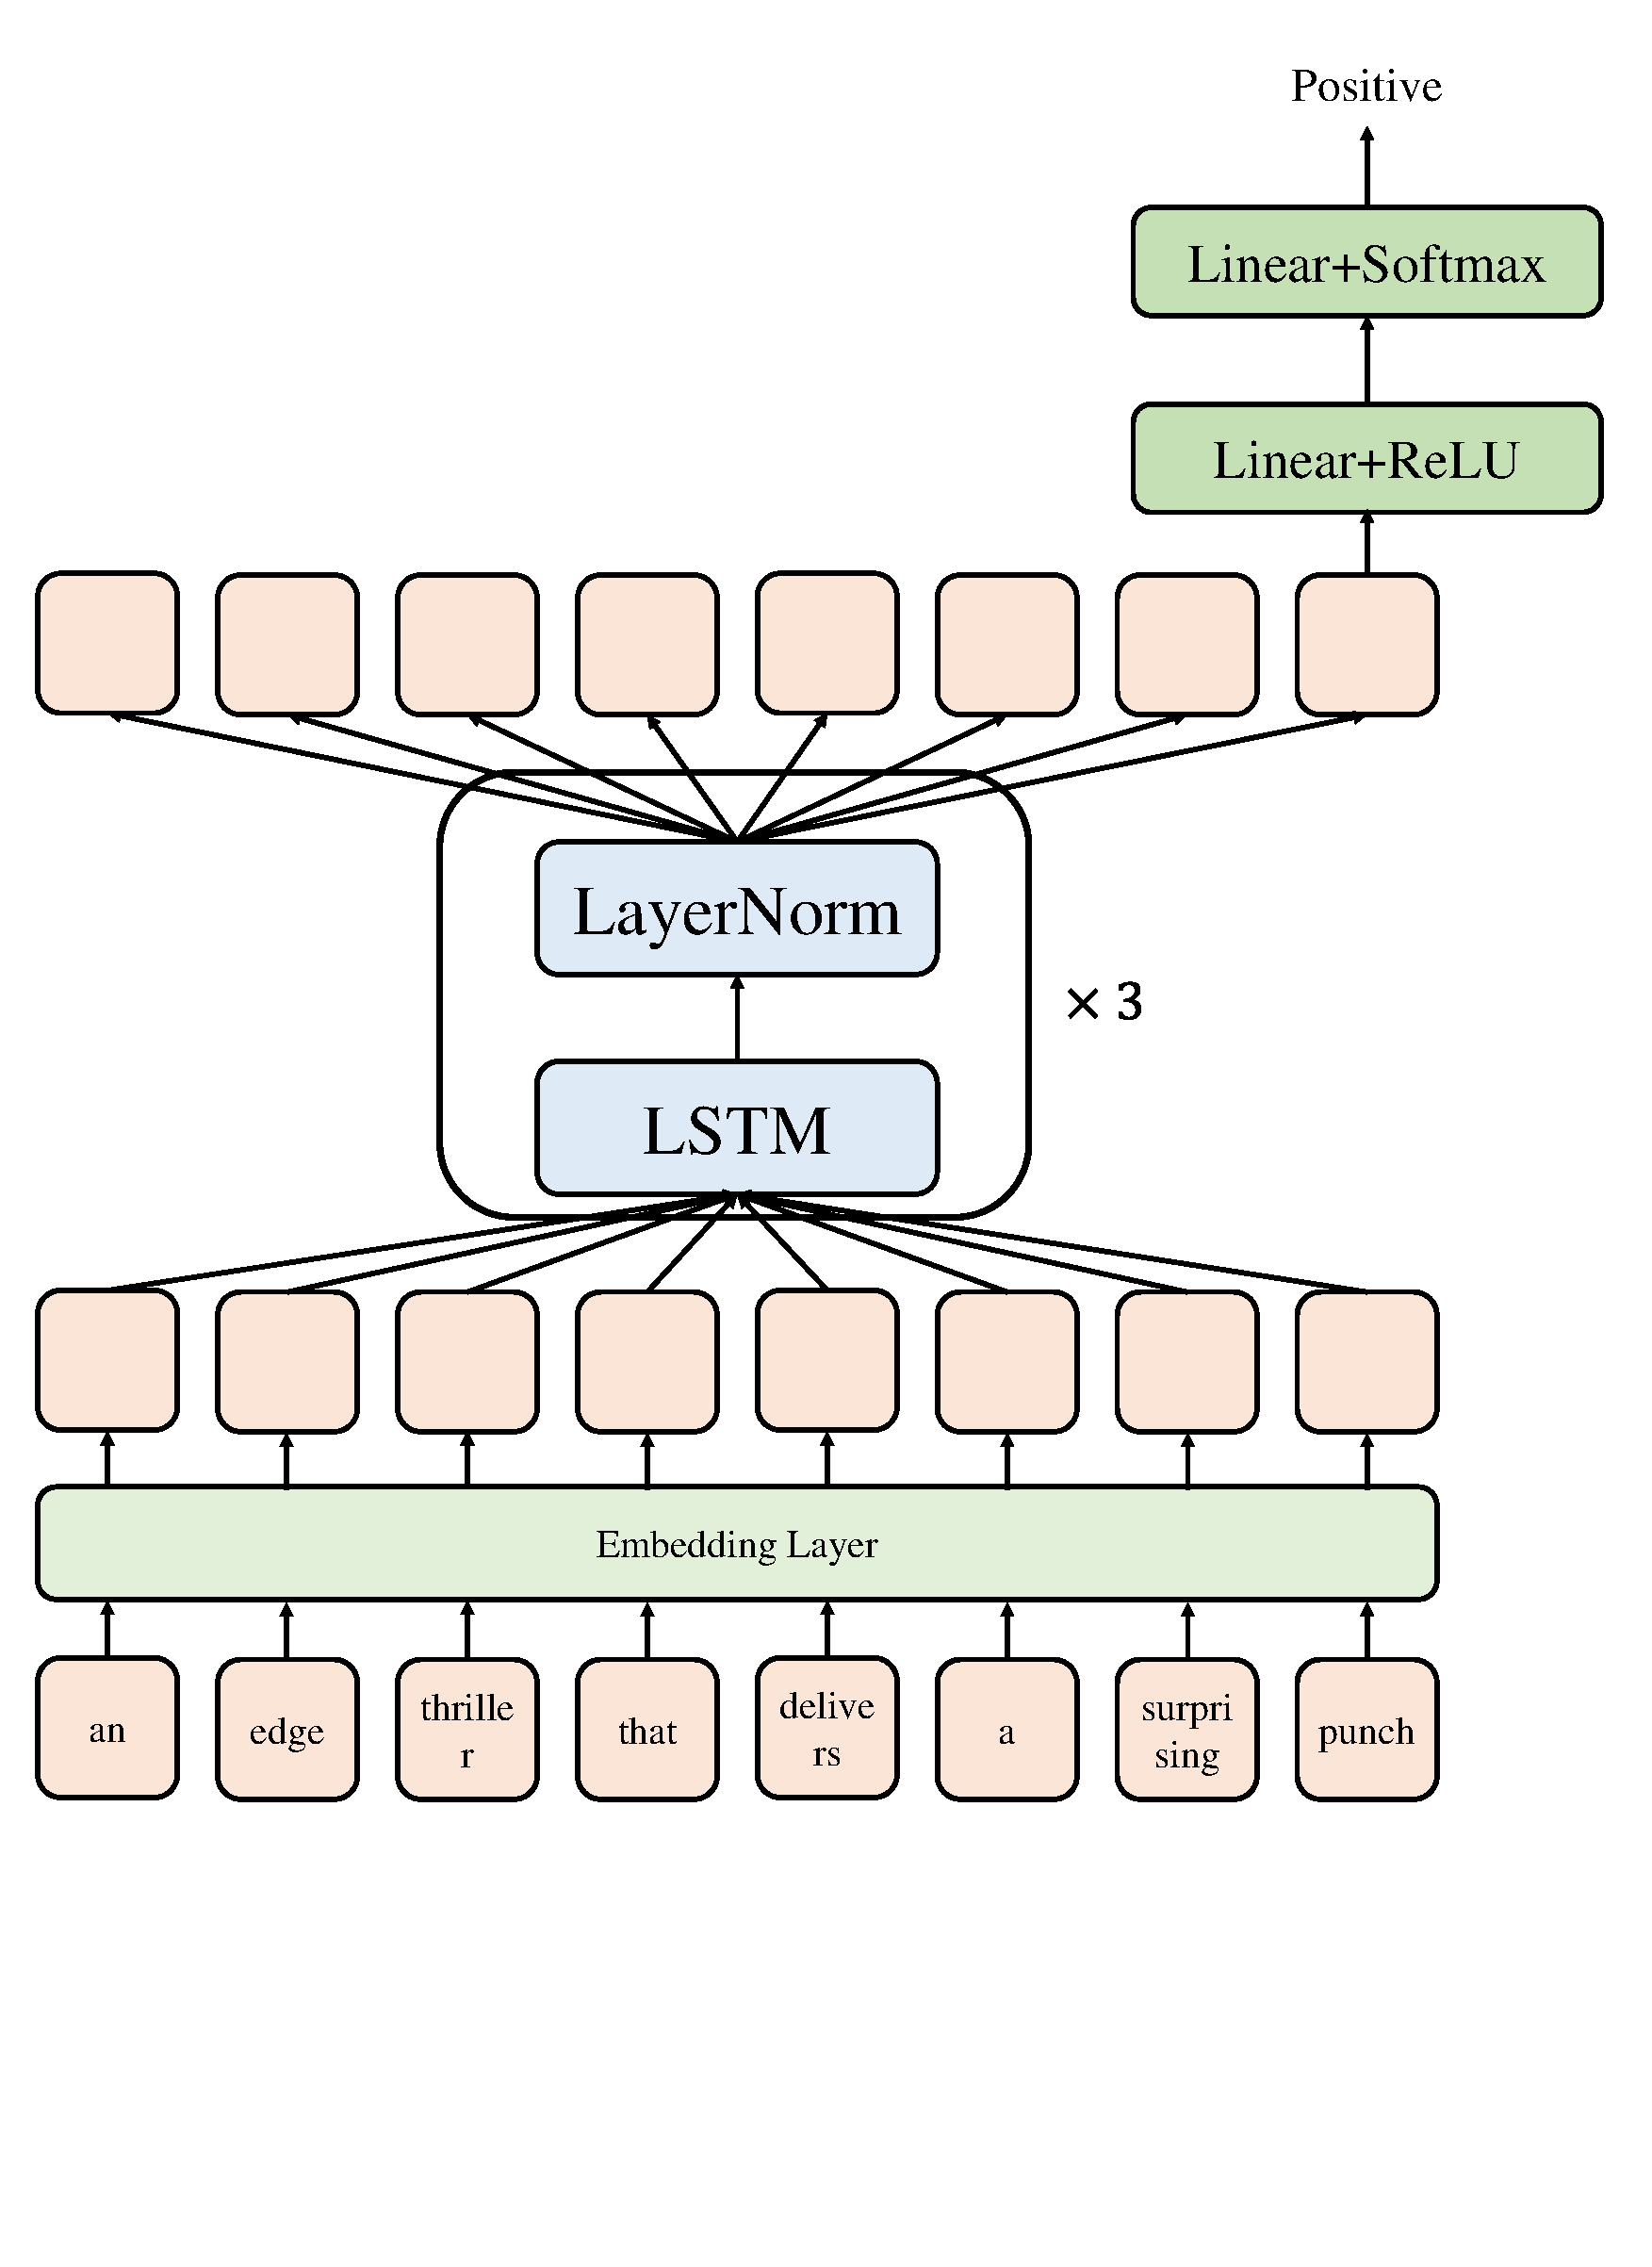
\includegraphics[width=0.5\textwidth]{lstm_model.pdf}
    \caption{Illustration of LSTM models.}
    \label{fig:lstm_model}
\end{figure}
\subsection{Model \& Hyperparameters}
The model framework is displayed at Fig.~\ref{fig:lstm_model}. I use three LSTM layers, three layer-normalization layers, two linear layers and a softmax classification layer. 
The reason for layer-normalization layer instead of batch-normalization layer is that words input are all padded with zero and not well-suitable for batch-normalization.
Because the last token stores all information from history, I use this token for classification.
The LSTM module is implemented by myself following the handout of Prof. Zhang.
In other words, I take the input sequence as the initial state of each LSTM block. And an all-zero tensor for initial hidden state.
In LSTM layer, the hidden state of each token of a sequence is incrementally updated from left to right.

\hspace*{\fill} \\
\noindent
I use 256 as the batch size and set each hidden state of LSTM layer to 512.
I ran the whole model for 105 epochs to ensure convergence.
The learning rate is set to $1\times 10^{-4}$ for stable training.
To make the model trainable, I first preprocess the dataset and precompute the longest sentence.
After that, I pad zero after other sentences that are shorter that the longest one.
I only sample 6920 sentences from the dataset and maintain the ratio of negative samples to positive samples to be nearly the same.
I split the dataset as training/validation/testing to 0.8/0.1/0.1, respectively.
Again I adopt 0.2 as the dropout rate to mitigate over-fitting.

\begin{figure}
    \centering
    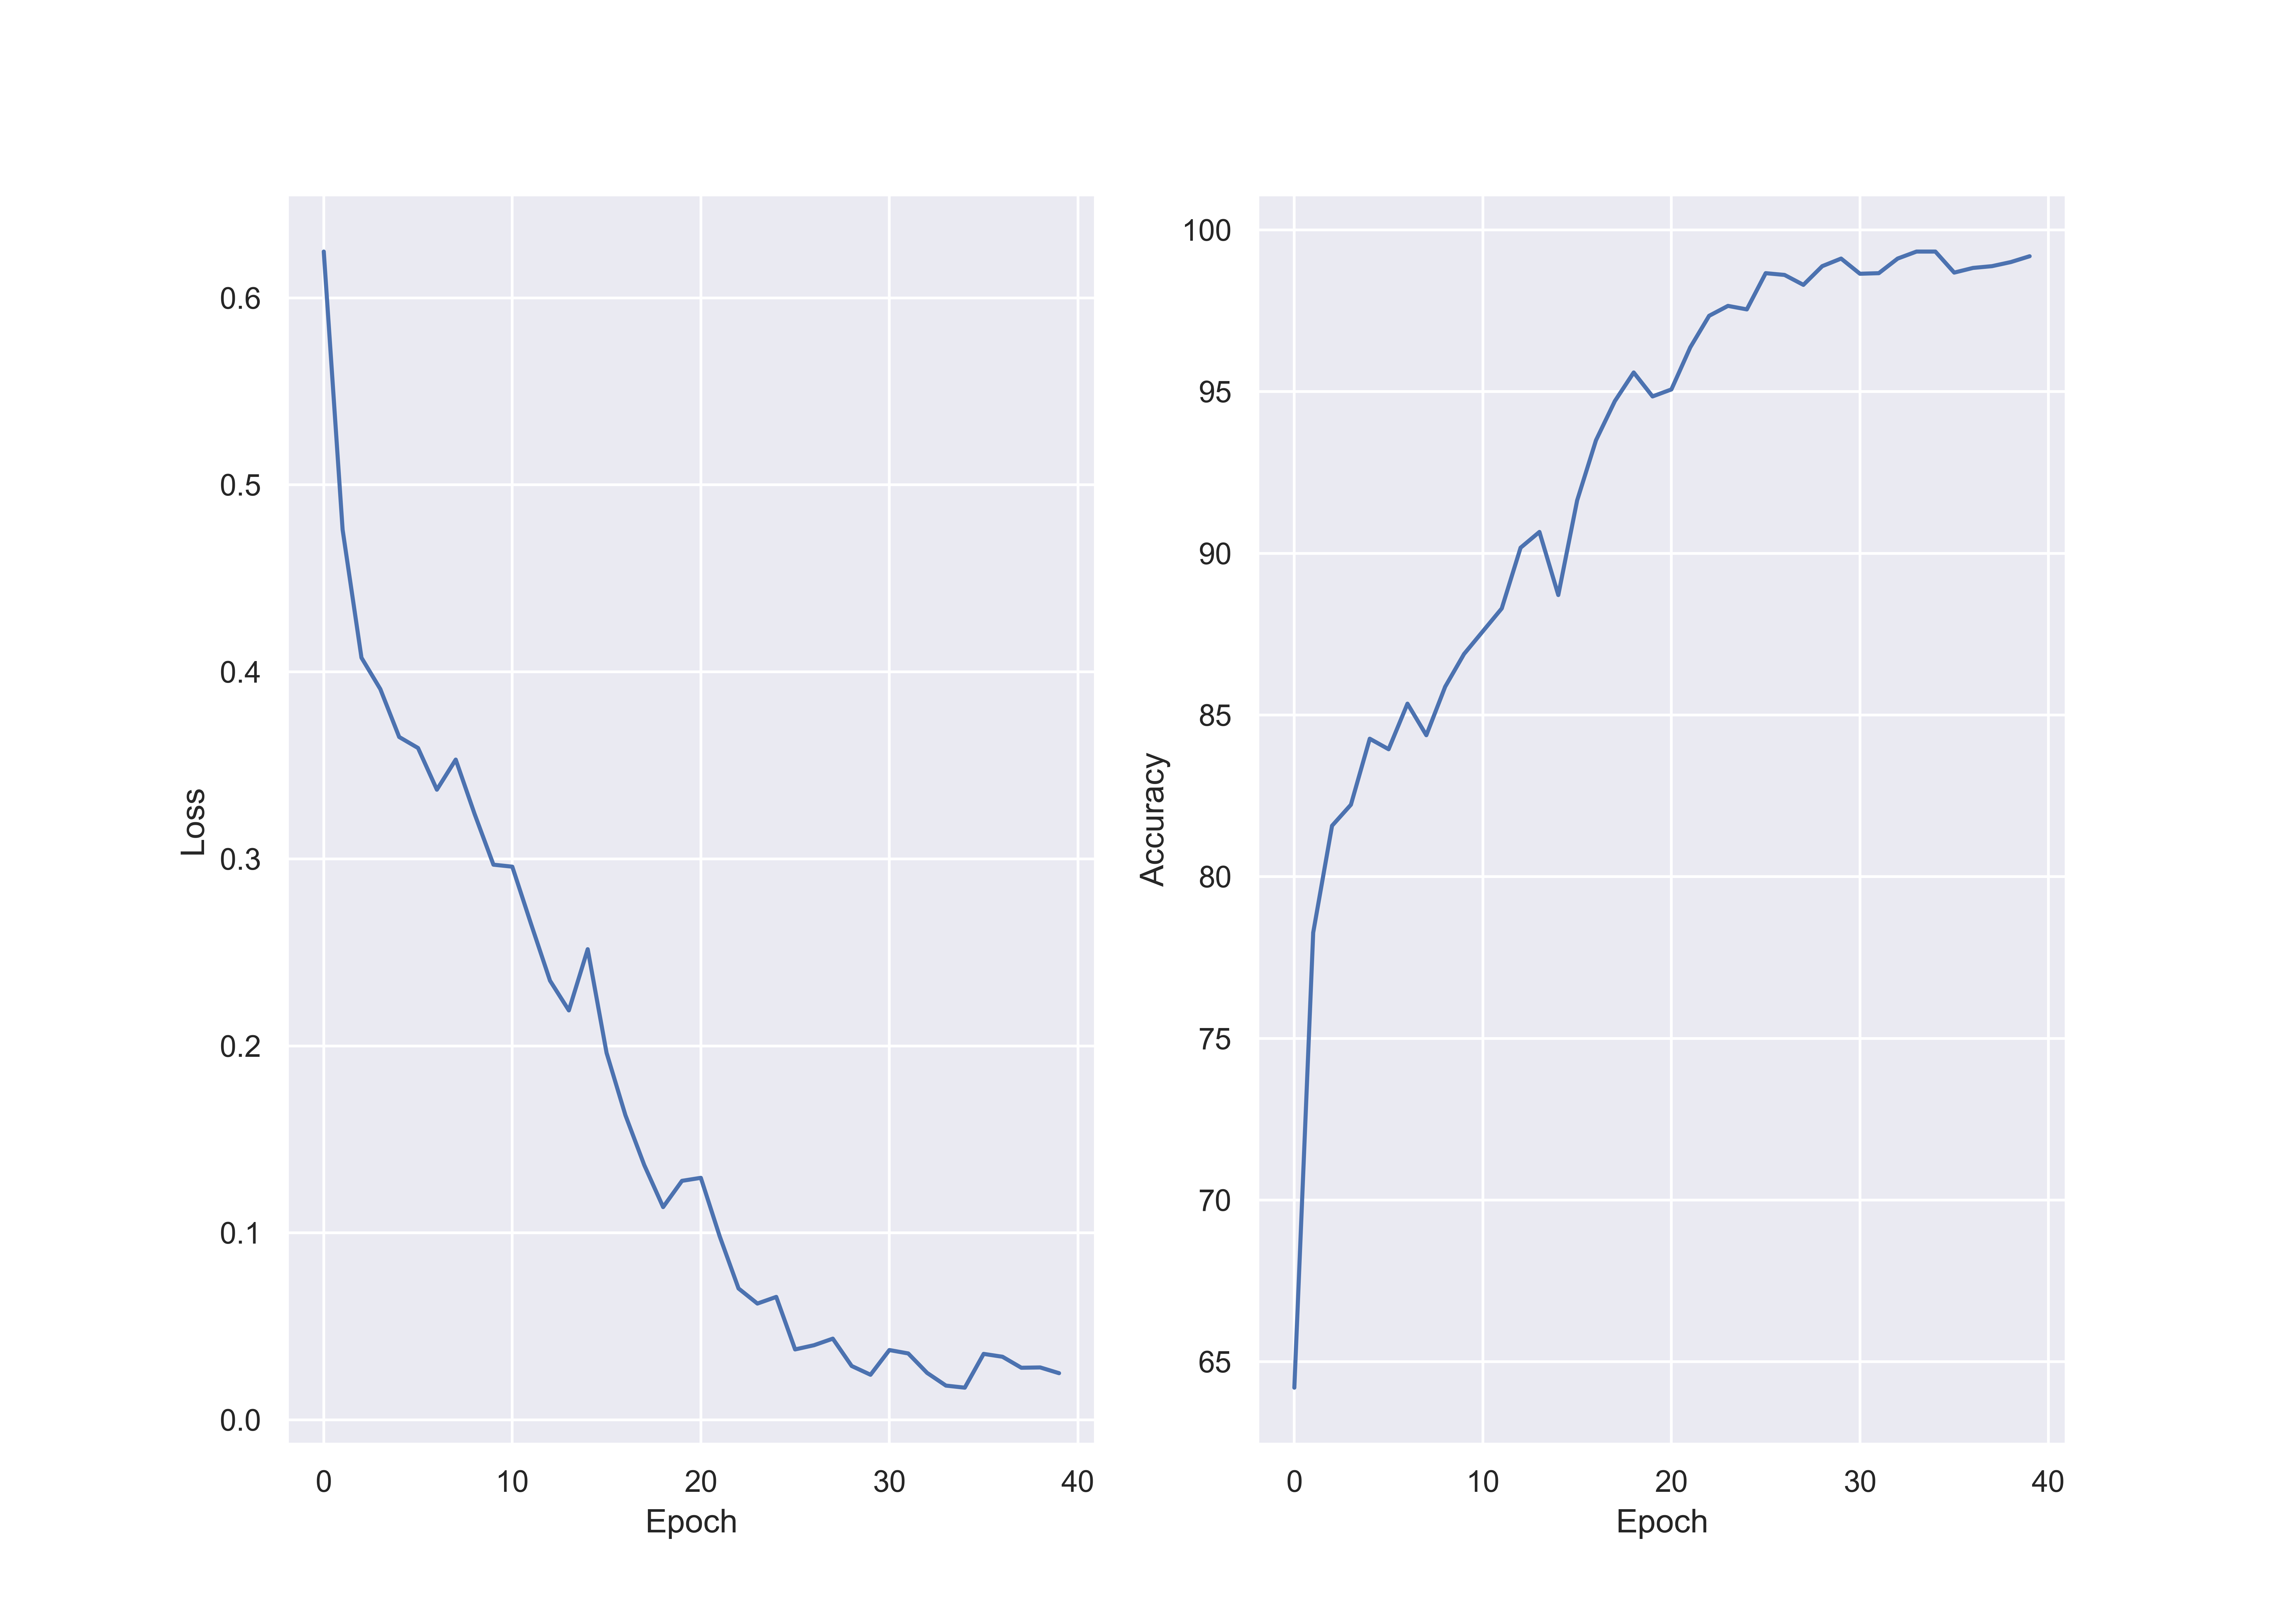
\includegraphics[width=0.8\linewidth]{../images/sst2-train-loss-acc.png}
    \caption{Change of training loss and accuracy in SST-2 dataset.}
    \label{fig:sst-train_loss}
\end{figure}
\begin{figure}
    \centering
    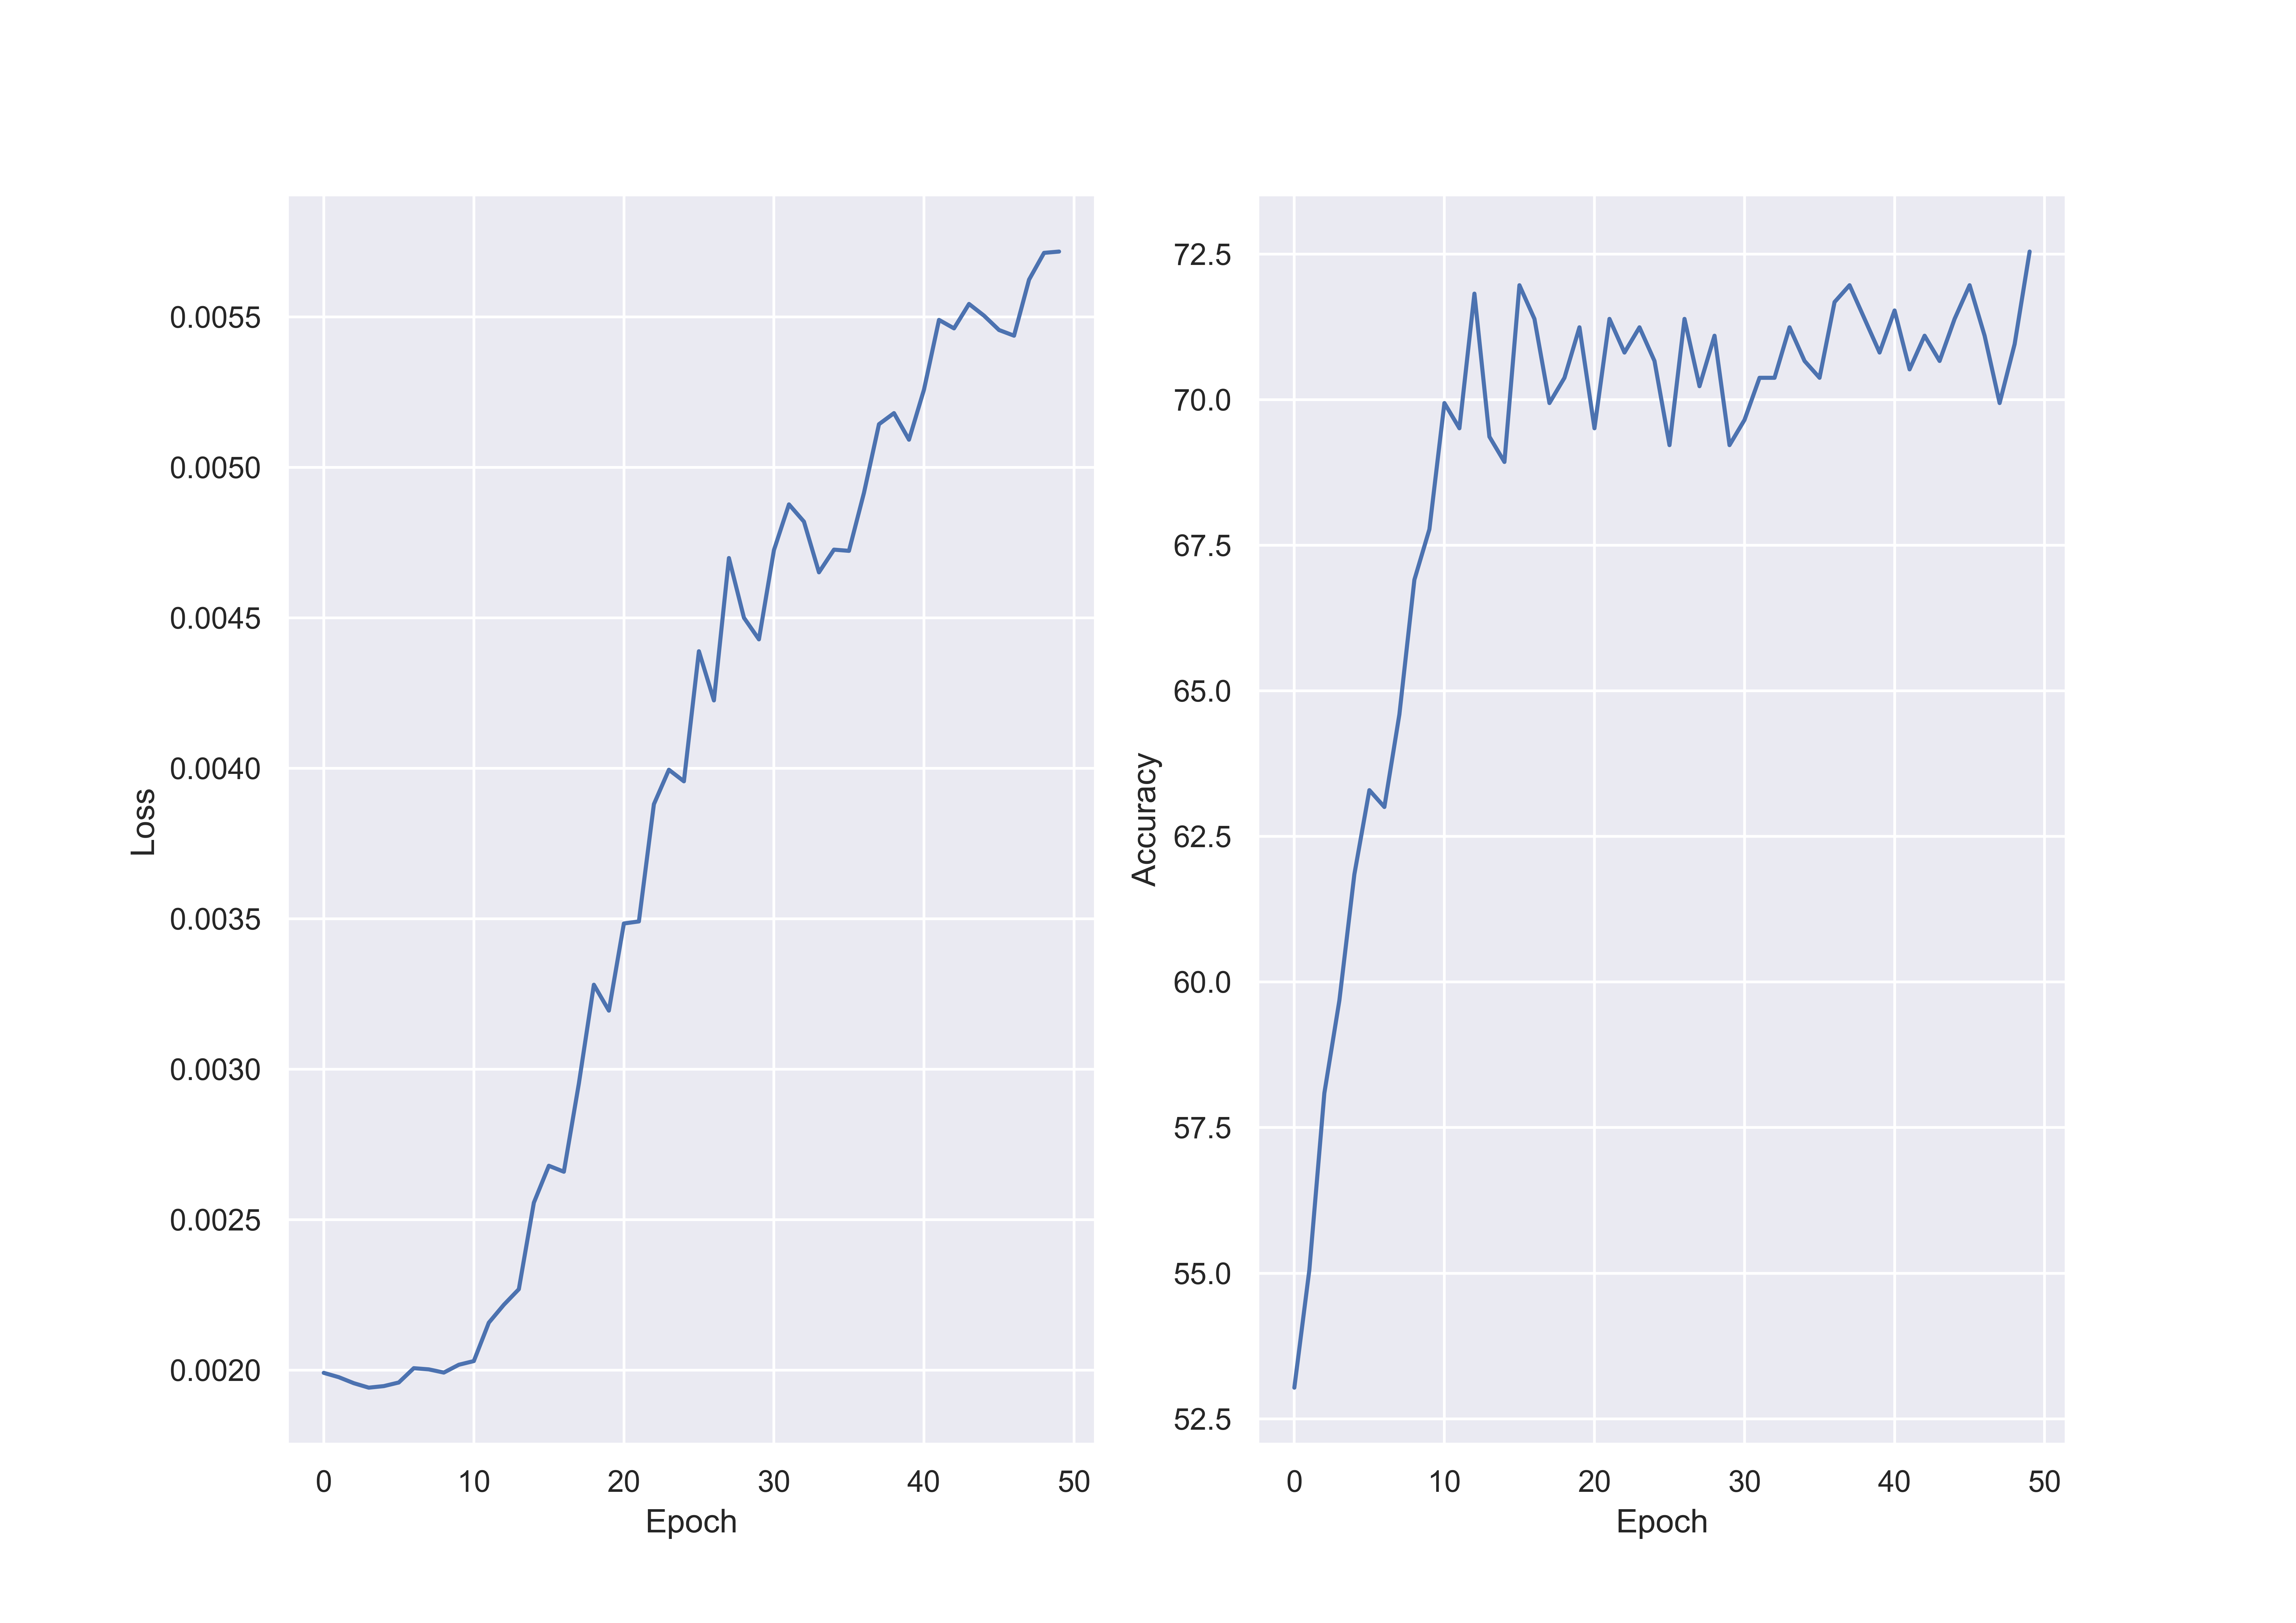
\includegraphics[width=0.8\linewidth]{../images/sst2-dev-loss-acc.png}
    \caption{Change of validation loss and accuracy in SST-2 dataset.}
    \label{fig:sst-dev_loss}
\end{figure}

\begin{figure}[htbp]
    \centering
    \begin{subfigure}
        \centering
        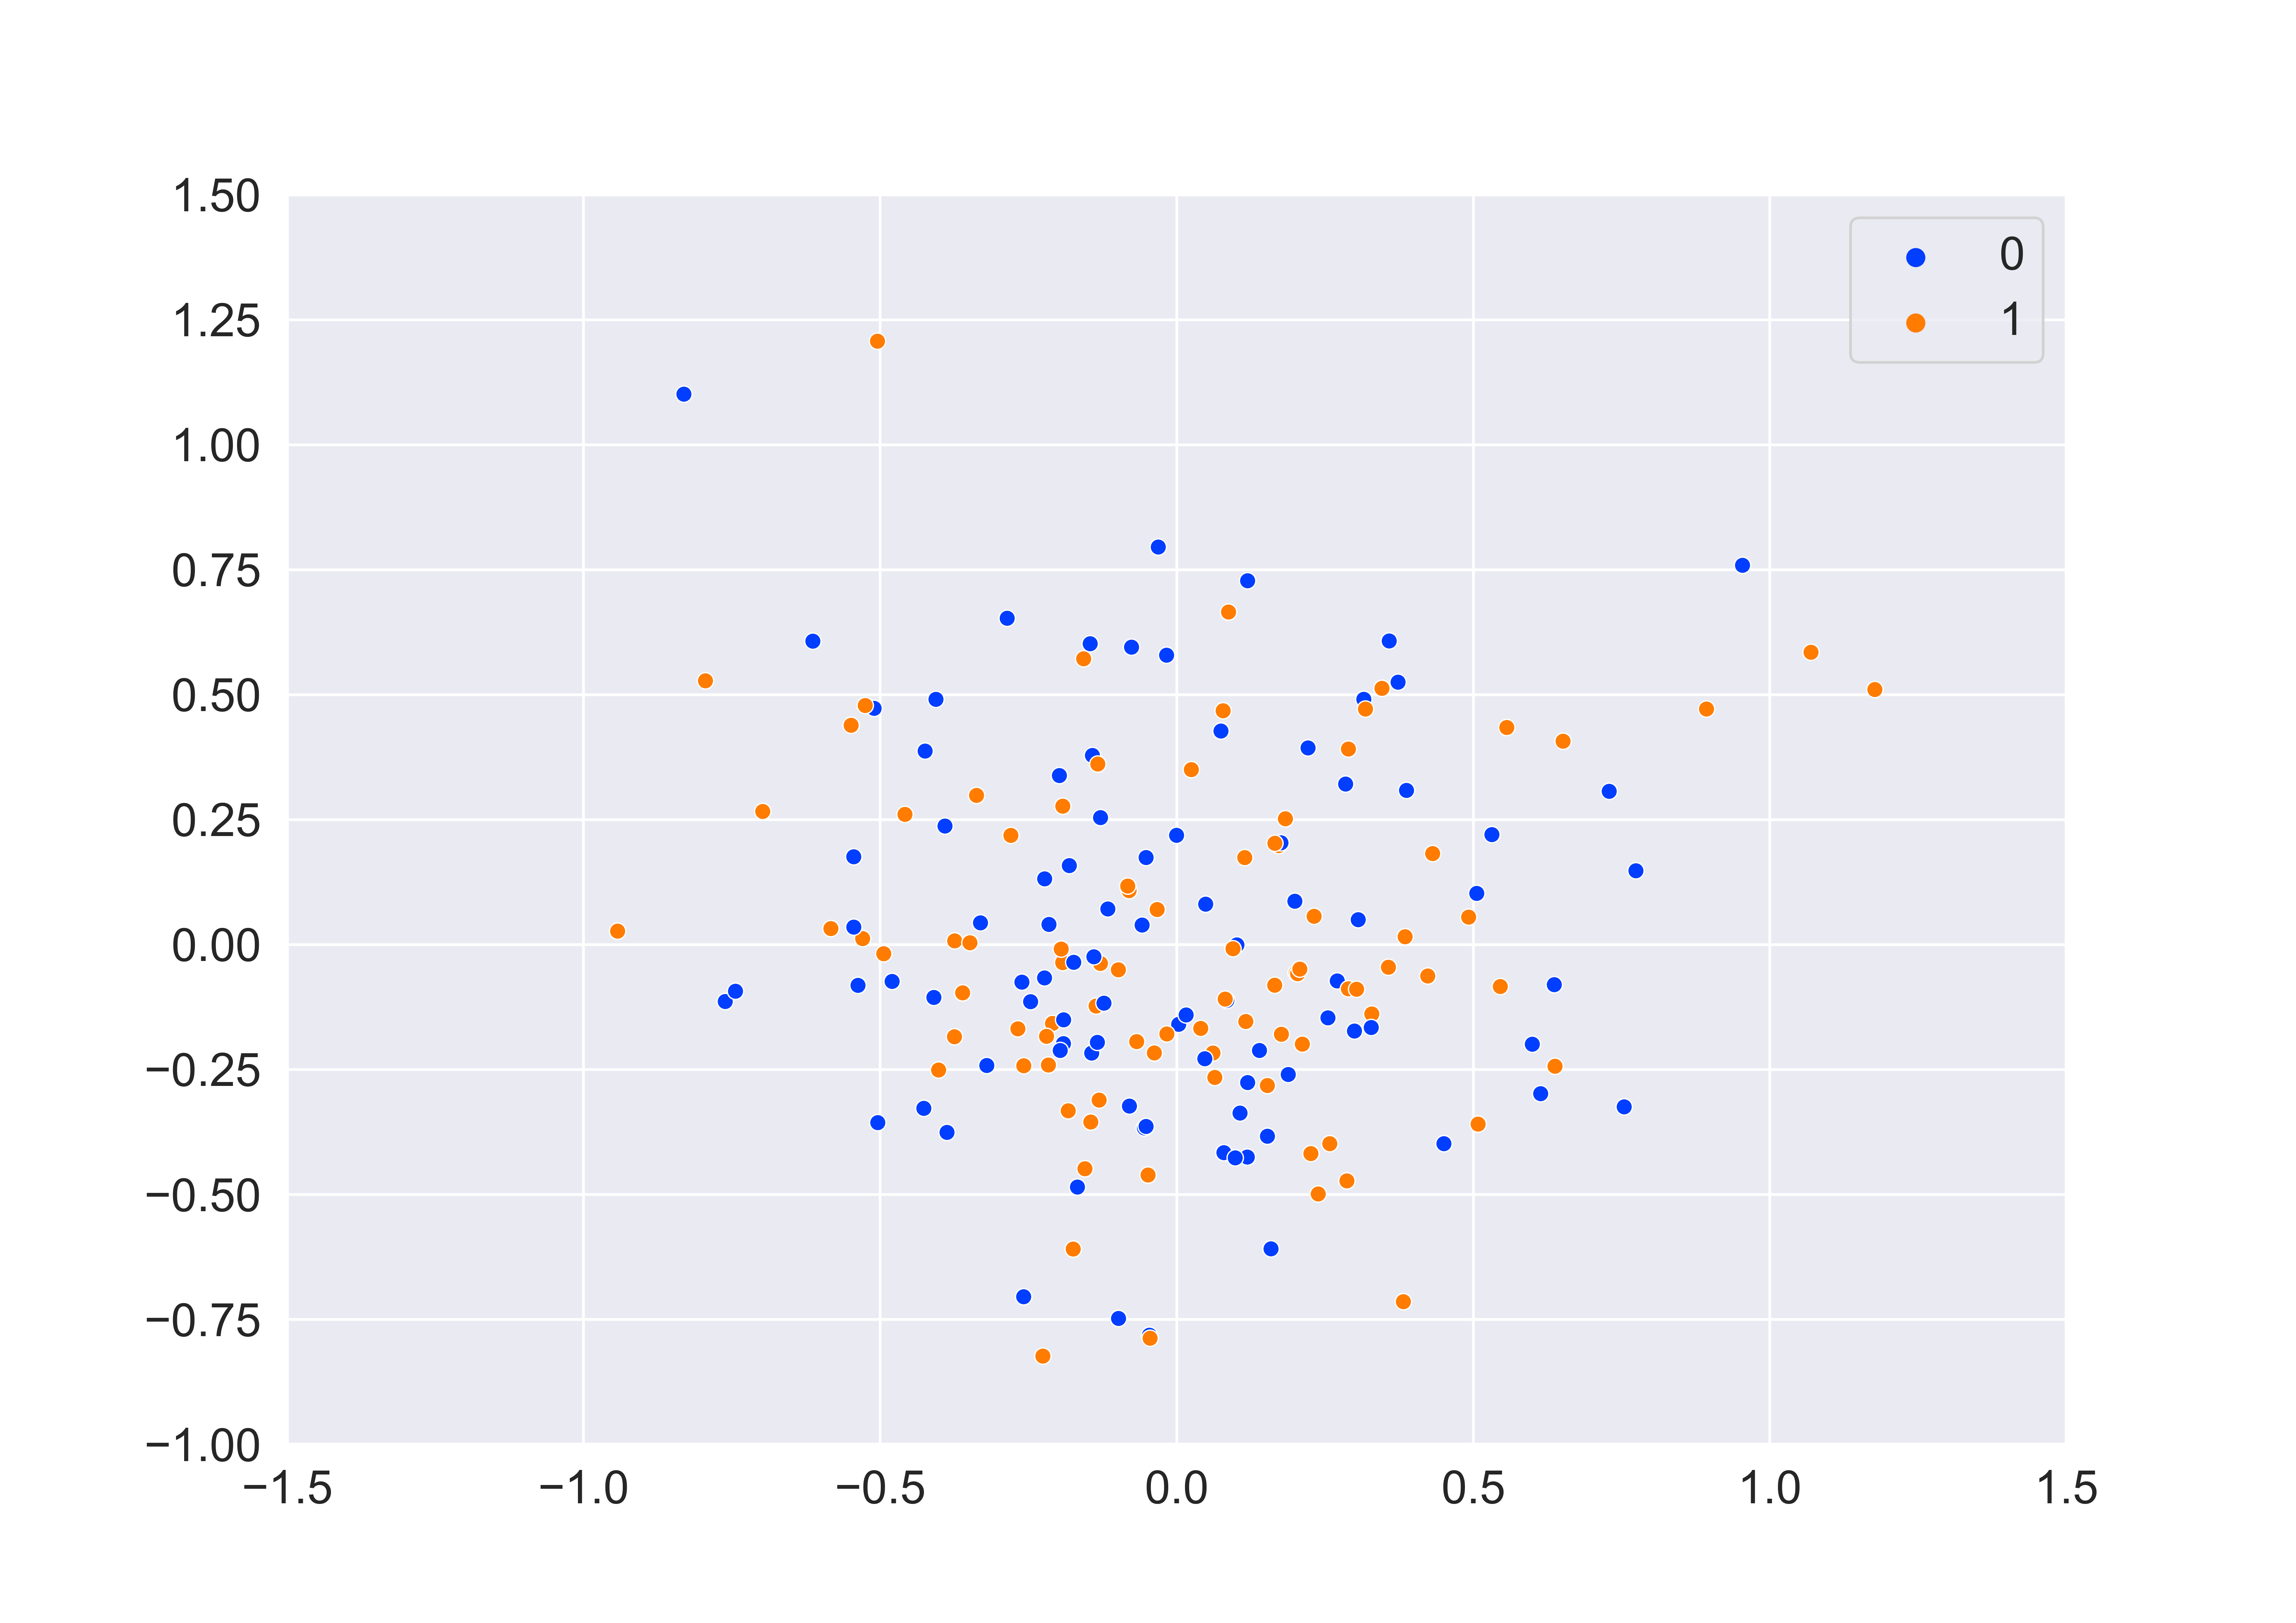
\includegraphics[width=0.45\linewidth]{../images/sst2_feature_map1_pca.png}
        % \caption{a}
        % \label{fig:mnist_tSNE_1}
    \end{subfigure}
    % \hfill 
    \begin{subfigure}
        \centering
        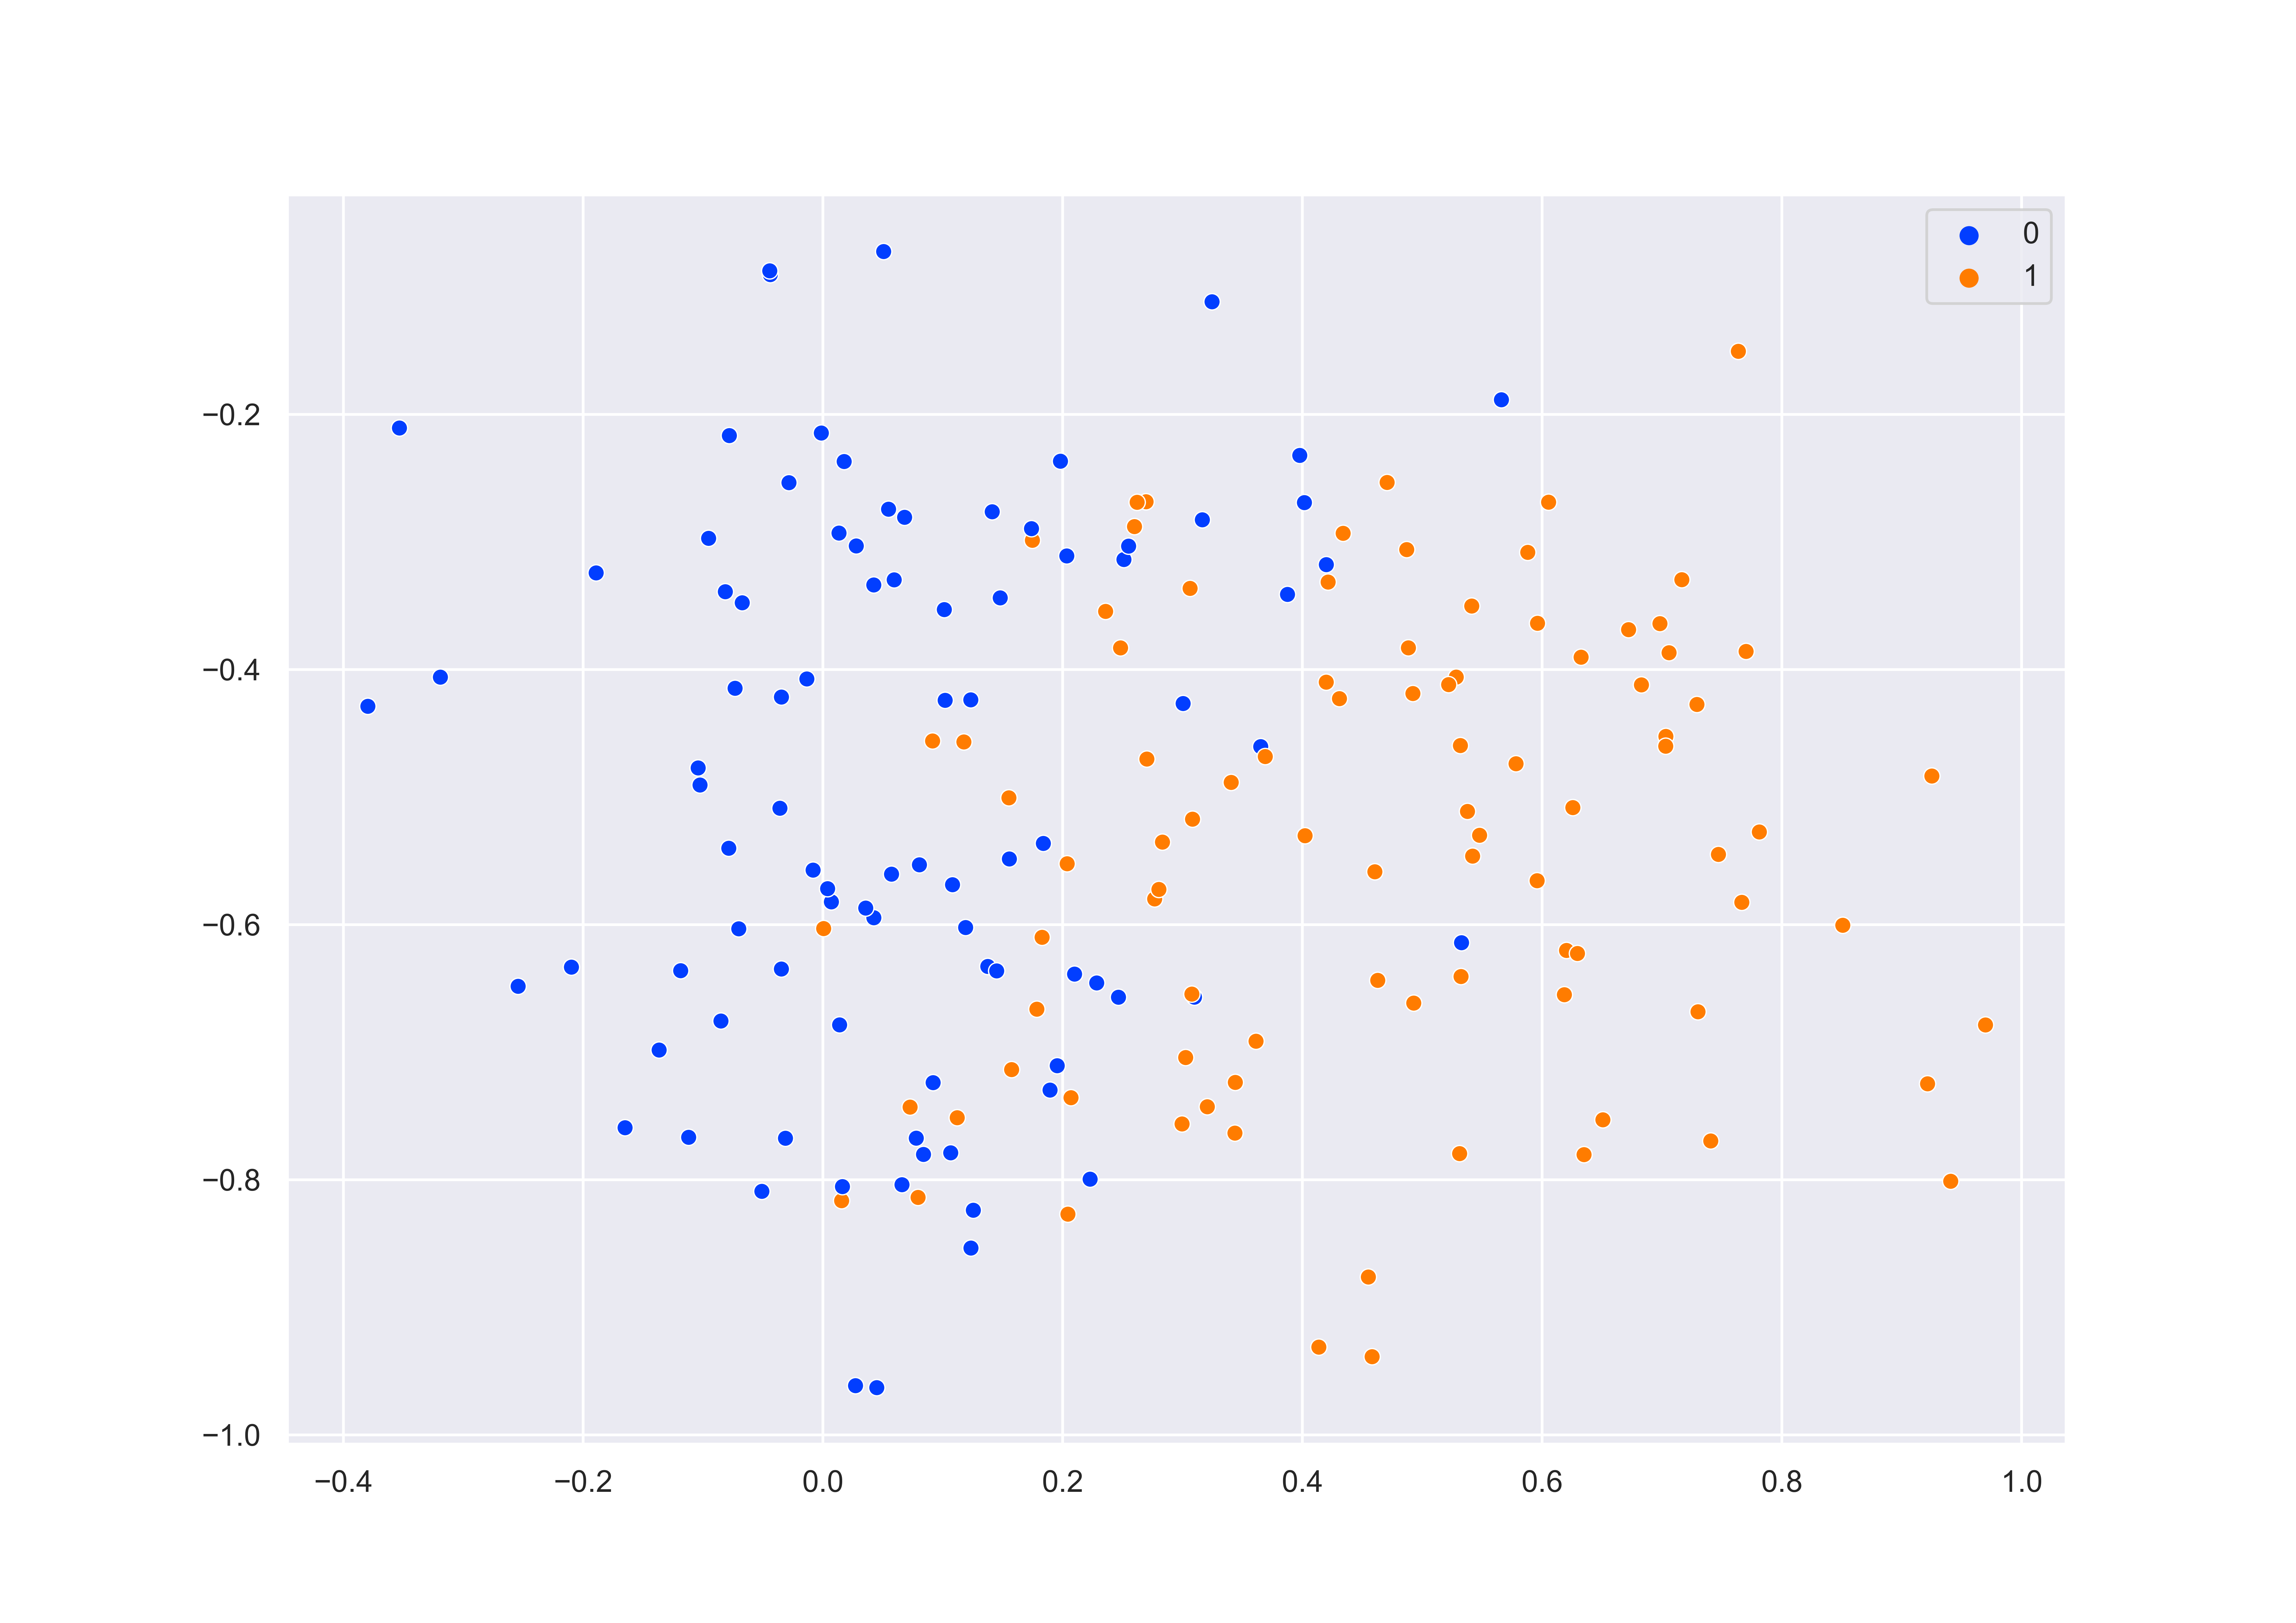
\includegraphics[width=0.45\linewidth]{../images/sst2_feature_map2_pca.png}
        % \caption{Absolute value of indivisual components of weight in ridge regression when setting $\lambda$ to 1.0.}
        % \label{fig:mnist_tSNE_2}
    \end{subfigure}
    % \hfill 
    \begin{subfigure}
        \centering
        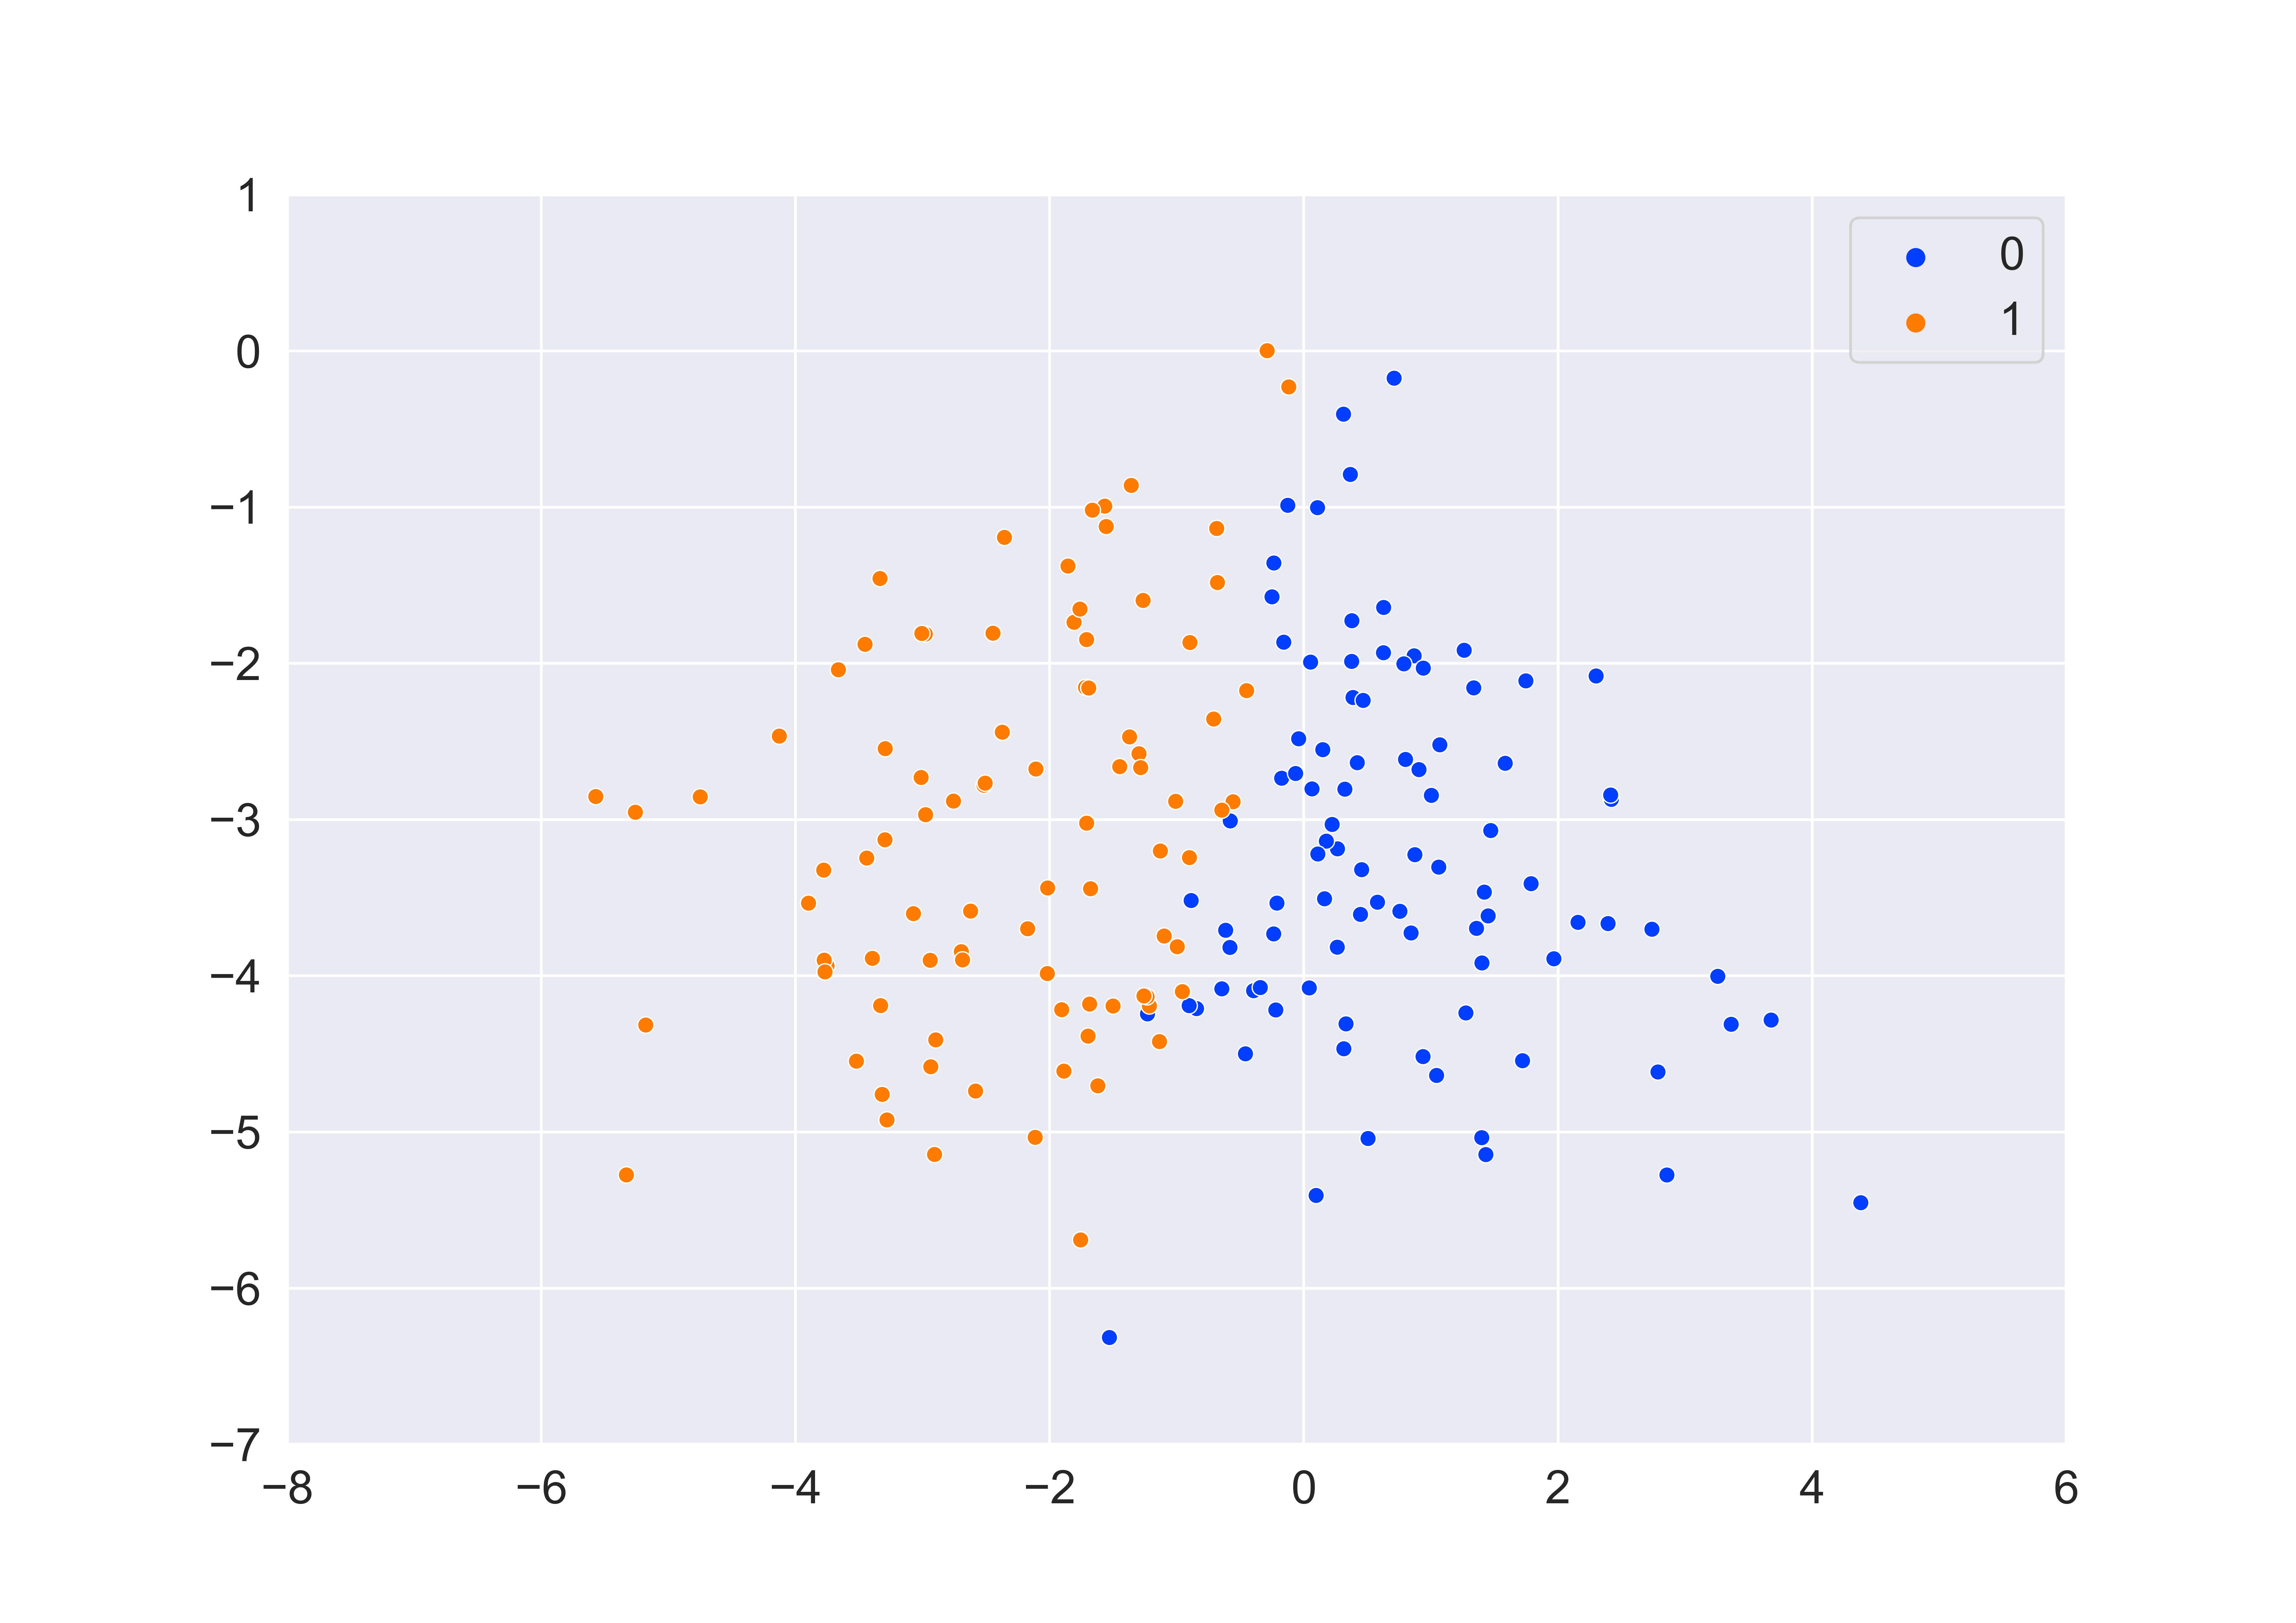
\includegraphics[width=0.45\linewidth]{../images/sst2_feature_map3_pca.png}
        % \caption{Absolute value of indivisual components of weight in ridge regression when setting $\lambda$ to 1.5.}
        % \label{fig:mnist_tSNE_3}
    \end{subfigure}
    \begin{subfigure}
        \centering
        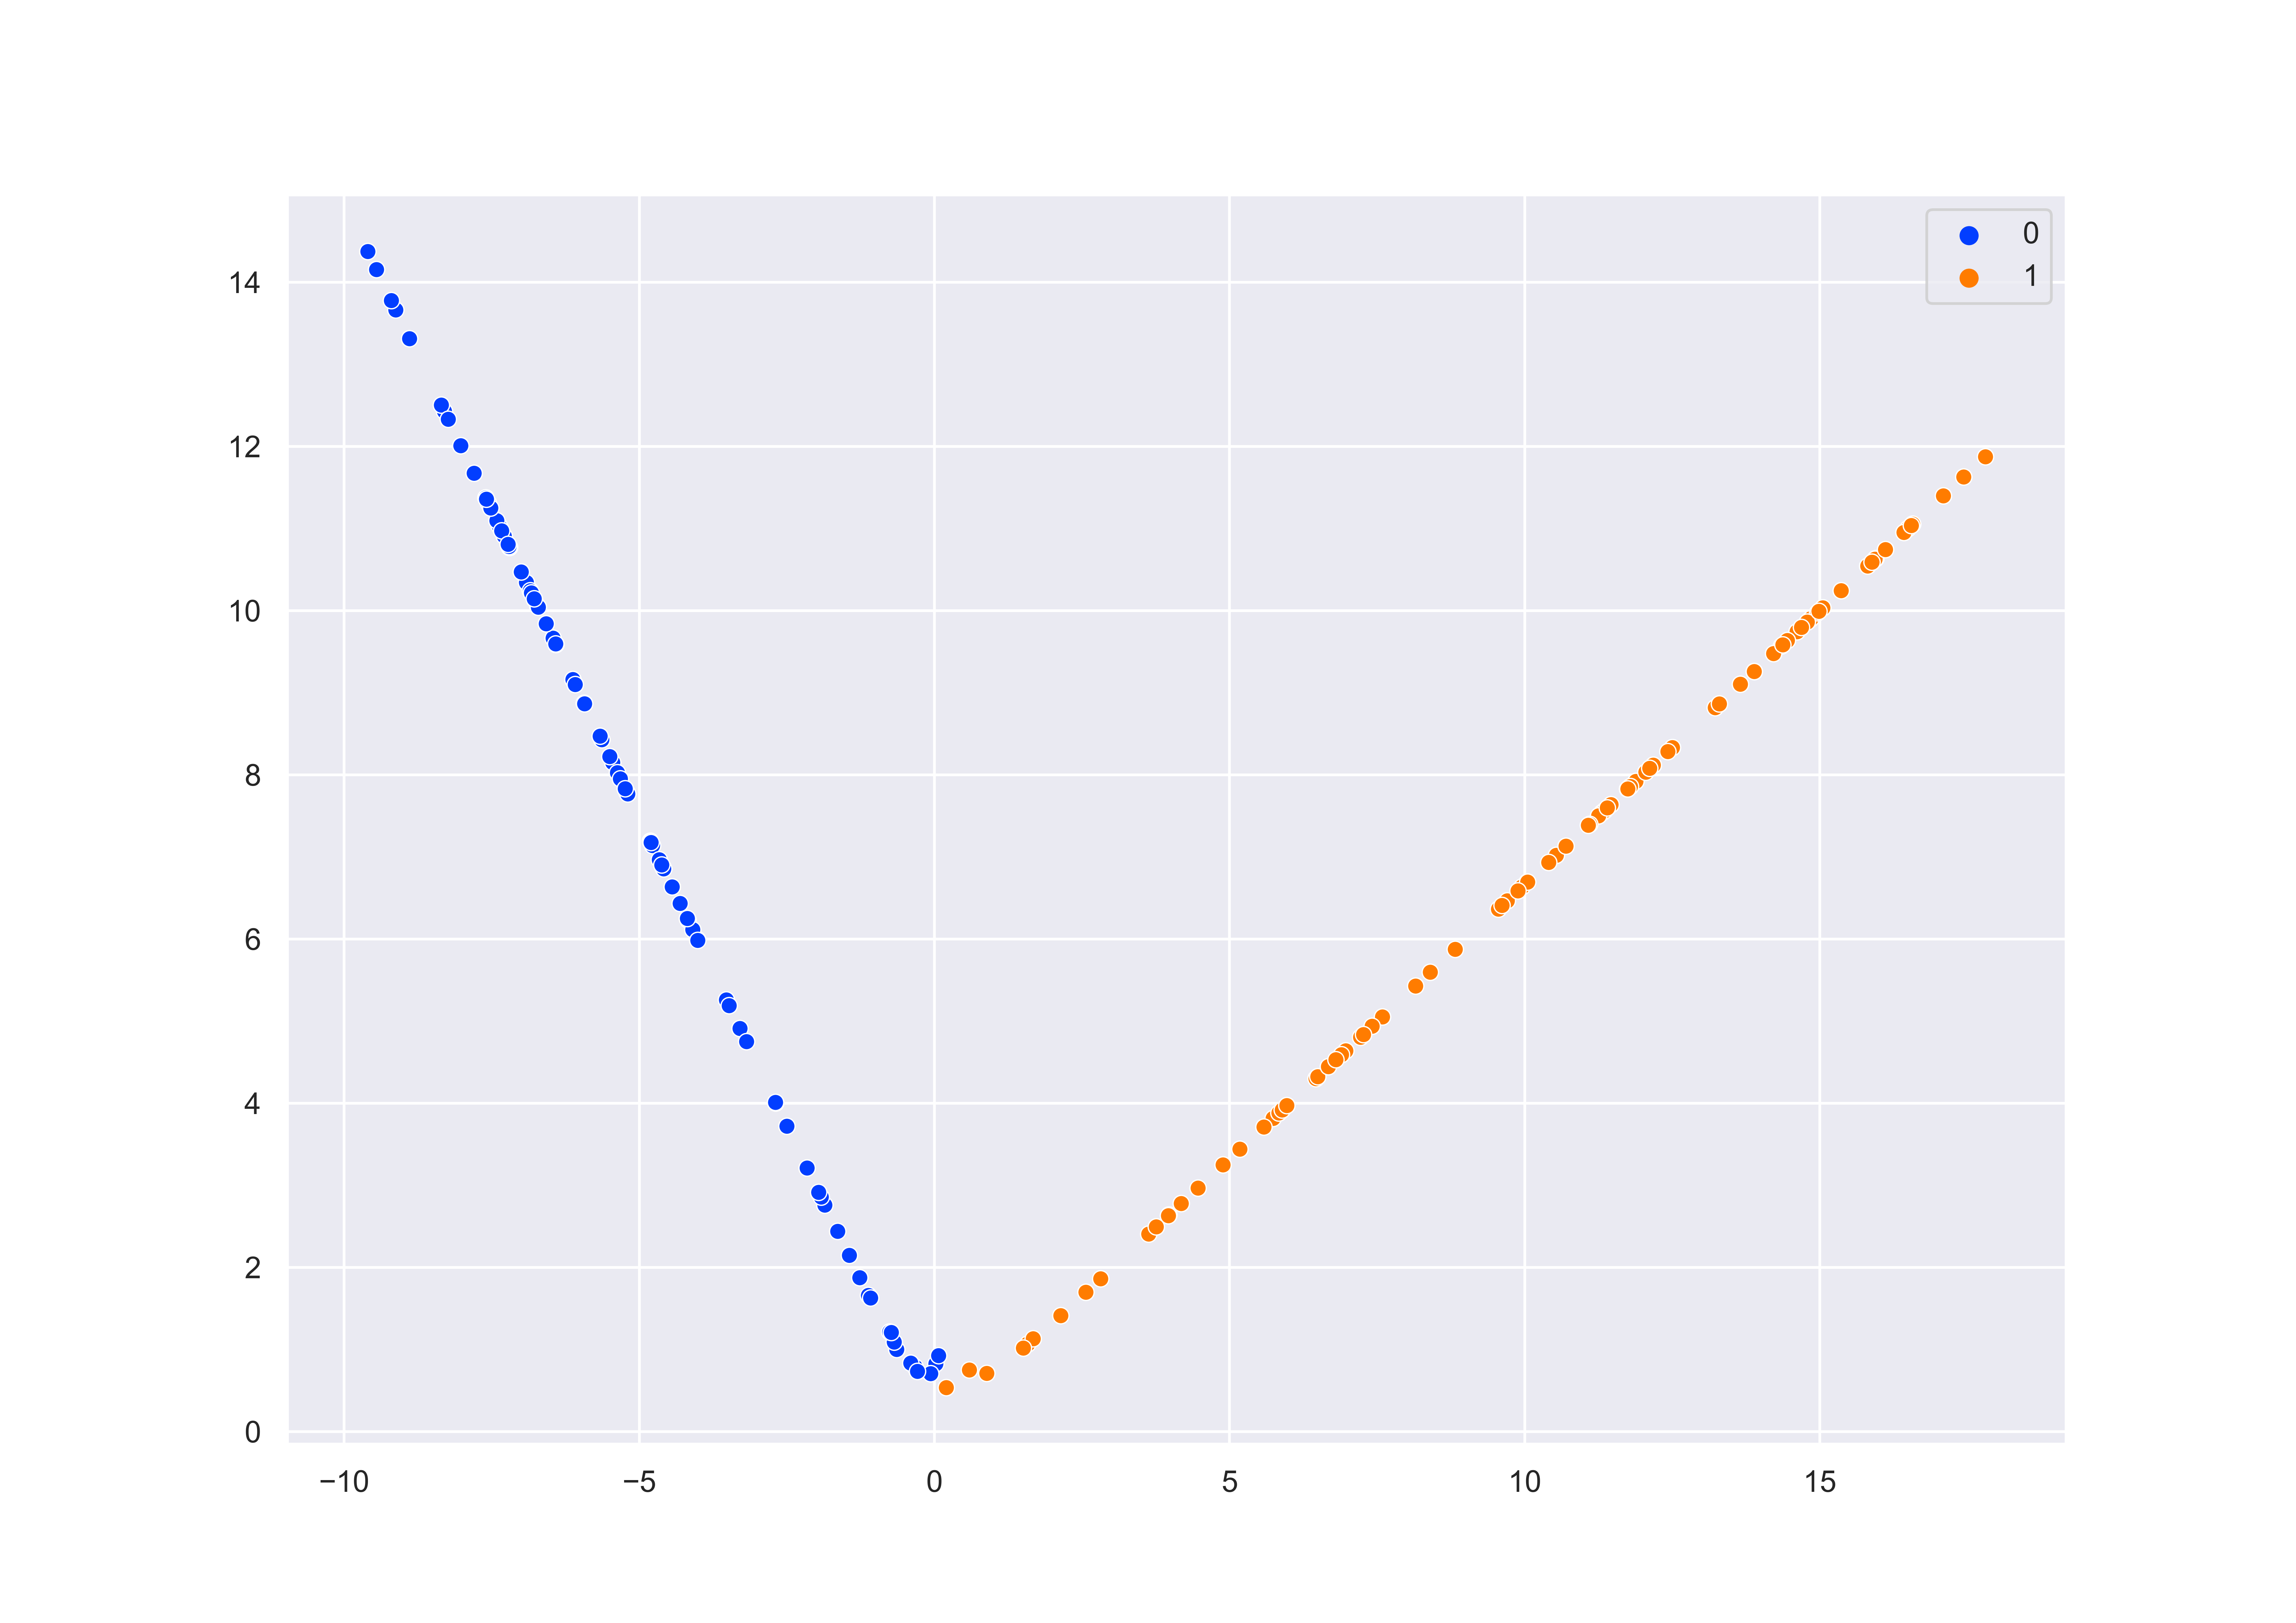
\includegraphics[width=0.45\linewidth]{../images/sst2_feature_map4_pca.png}
        % \caption{Absolute value of indivisual components of weight in ridge regression when setting $\lambda$ to 1.5.}
        % \label{fig:mnist_tSNE_3}
    \end{subfigure}
    \caption{Visualization images of intermediate output tensors with PCA method. Top-Left: Tensors after the first LSTM layer. Top-Right: Tensors after the second LSTM layer. Bottom-Left: Tensors after the final LSTM layer. Bottom-Right: Tensors after the first linear layer.}
    \label{fig:sst_pca}
\end{figure}

\begin{figure}[htbp]
    \centering
    \begin{subfigure}
        \centering
        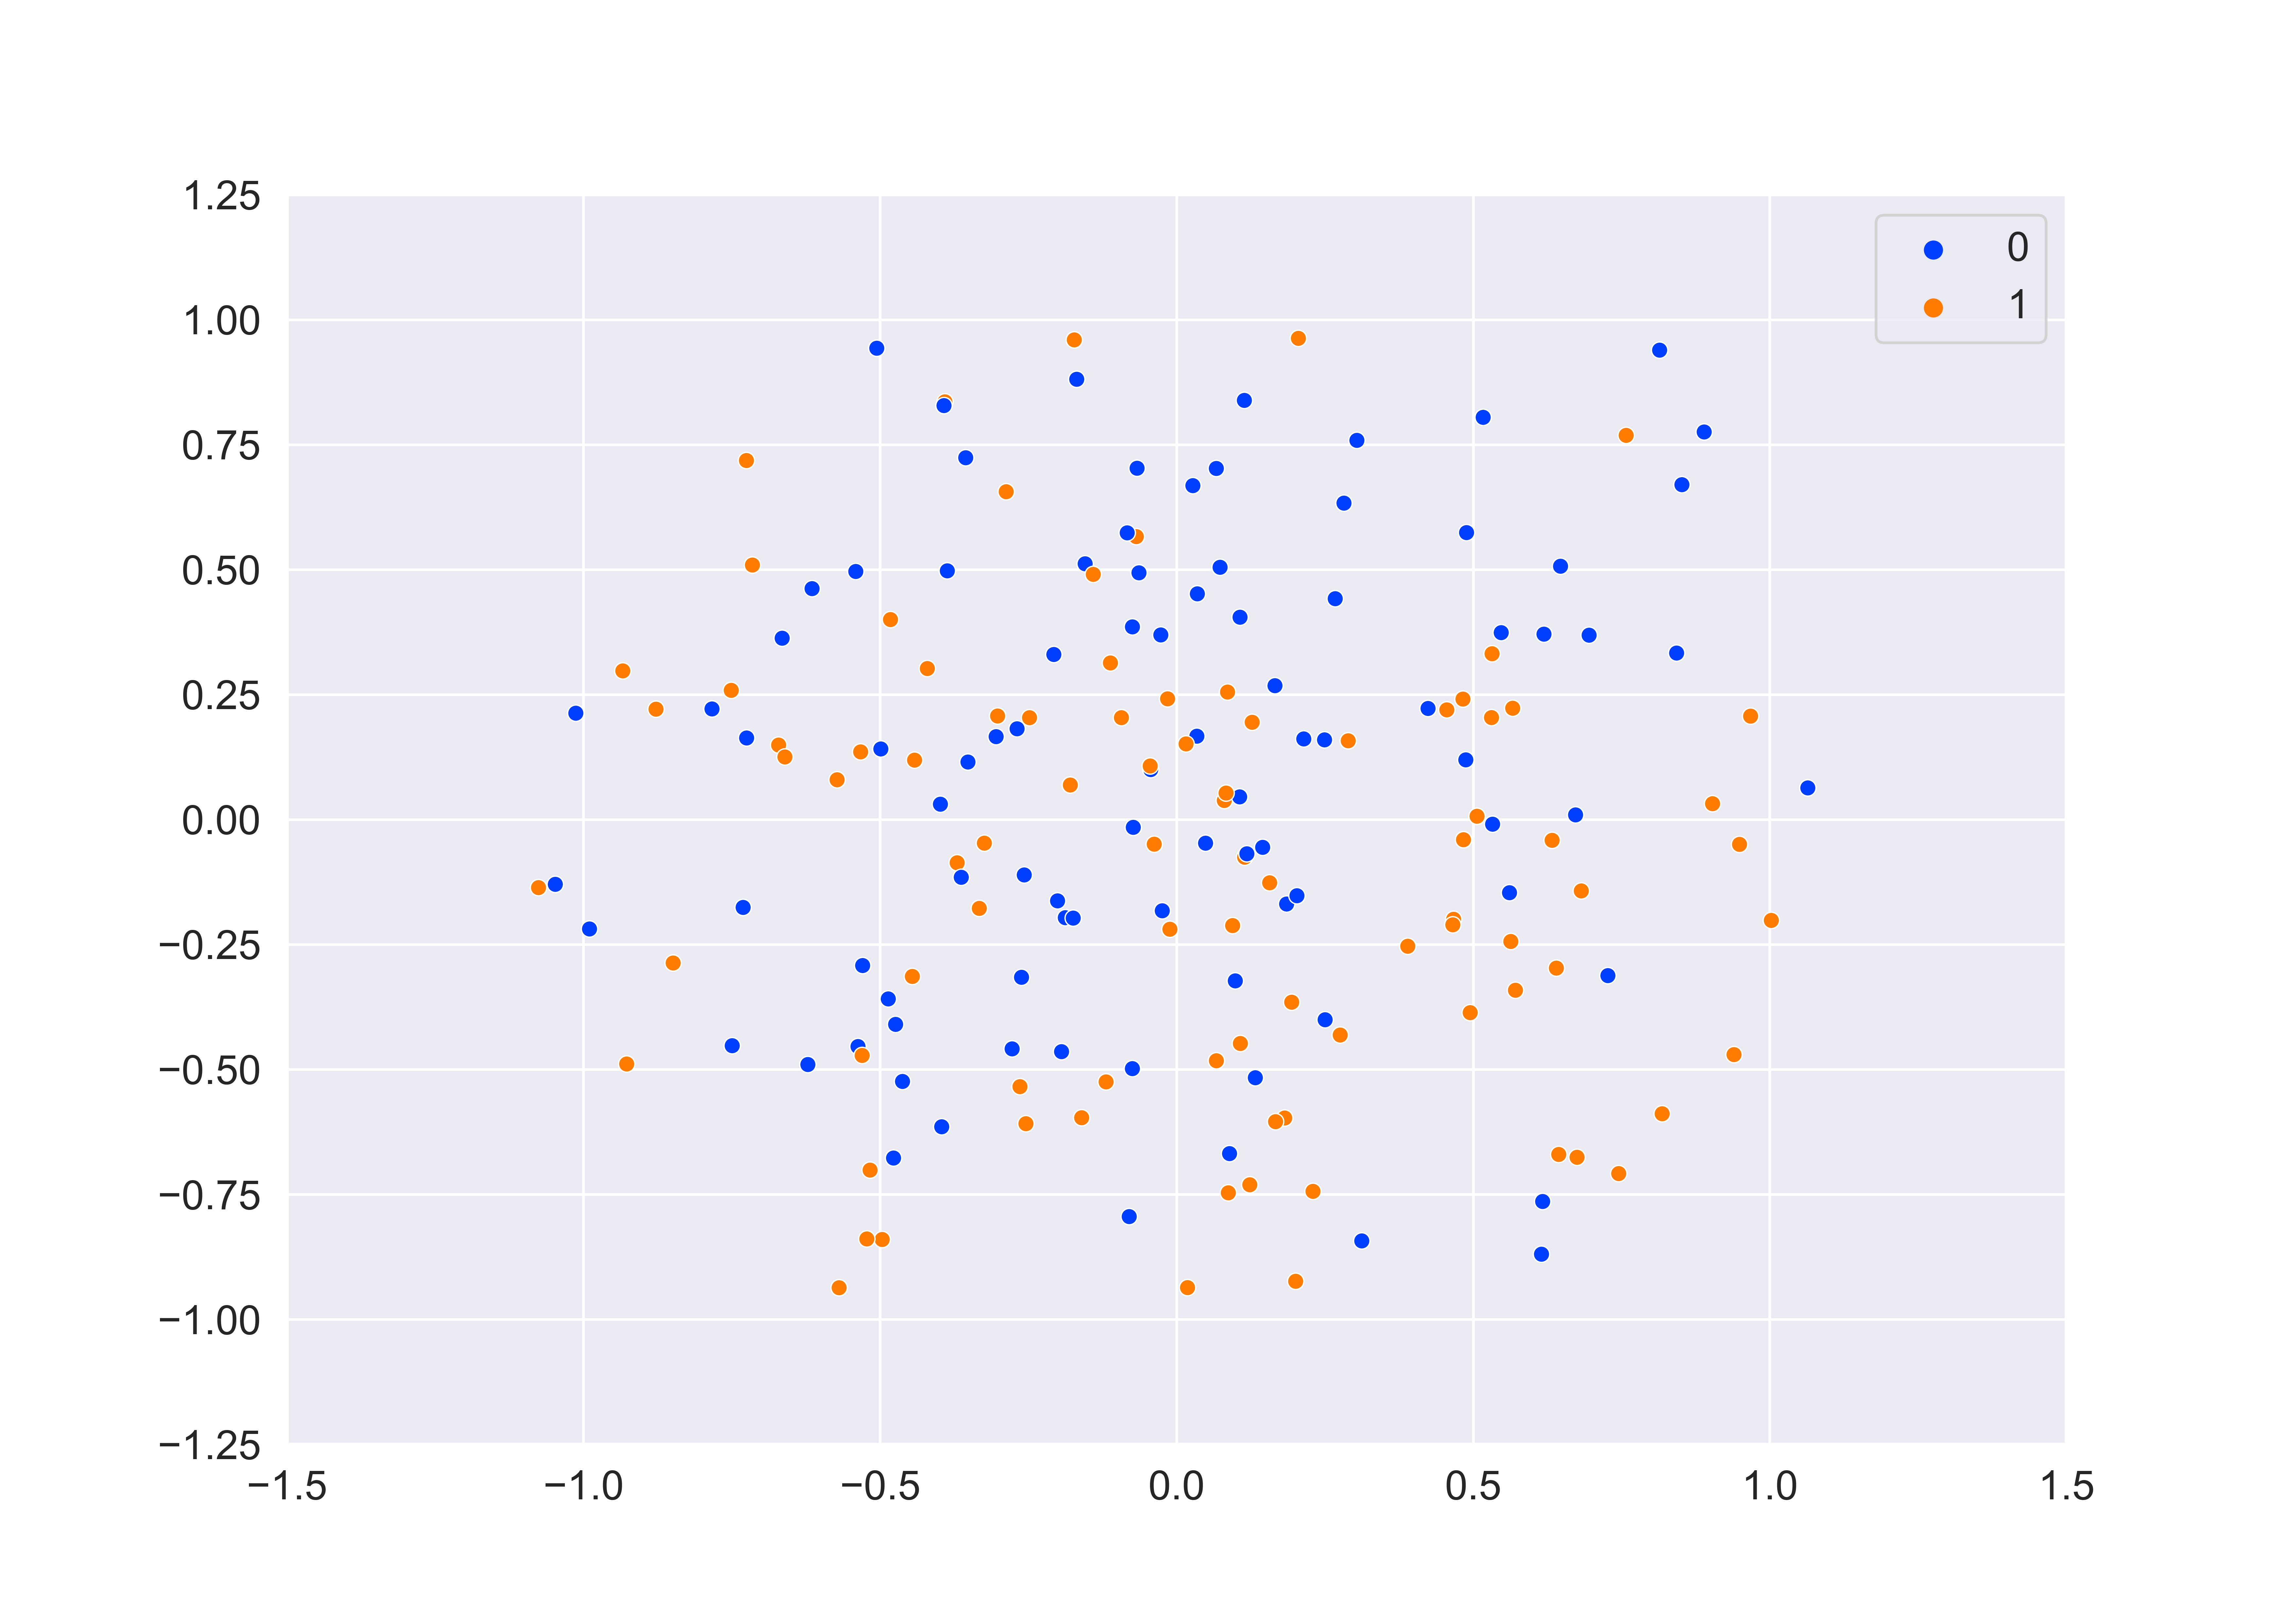
\includegraphics[width=0.45\linewidth]{../images/sst2_feature_map1_tsne.png}
        % \caption{a}
        % \label{fig:mnist_tSNE_1}
    \end{subfigure}
    % \hfill 
    \begin{subfigure}
        \centering
        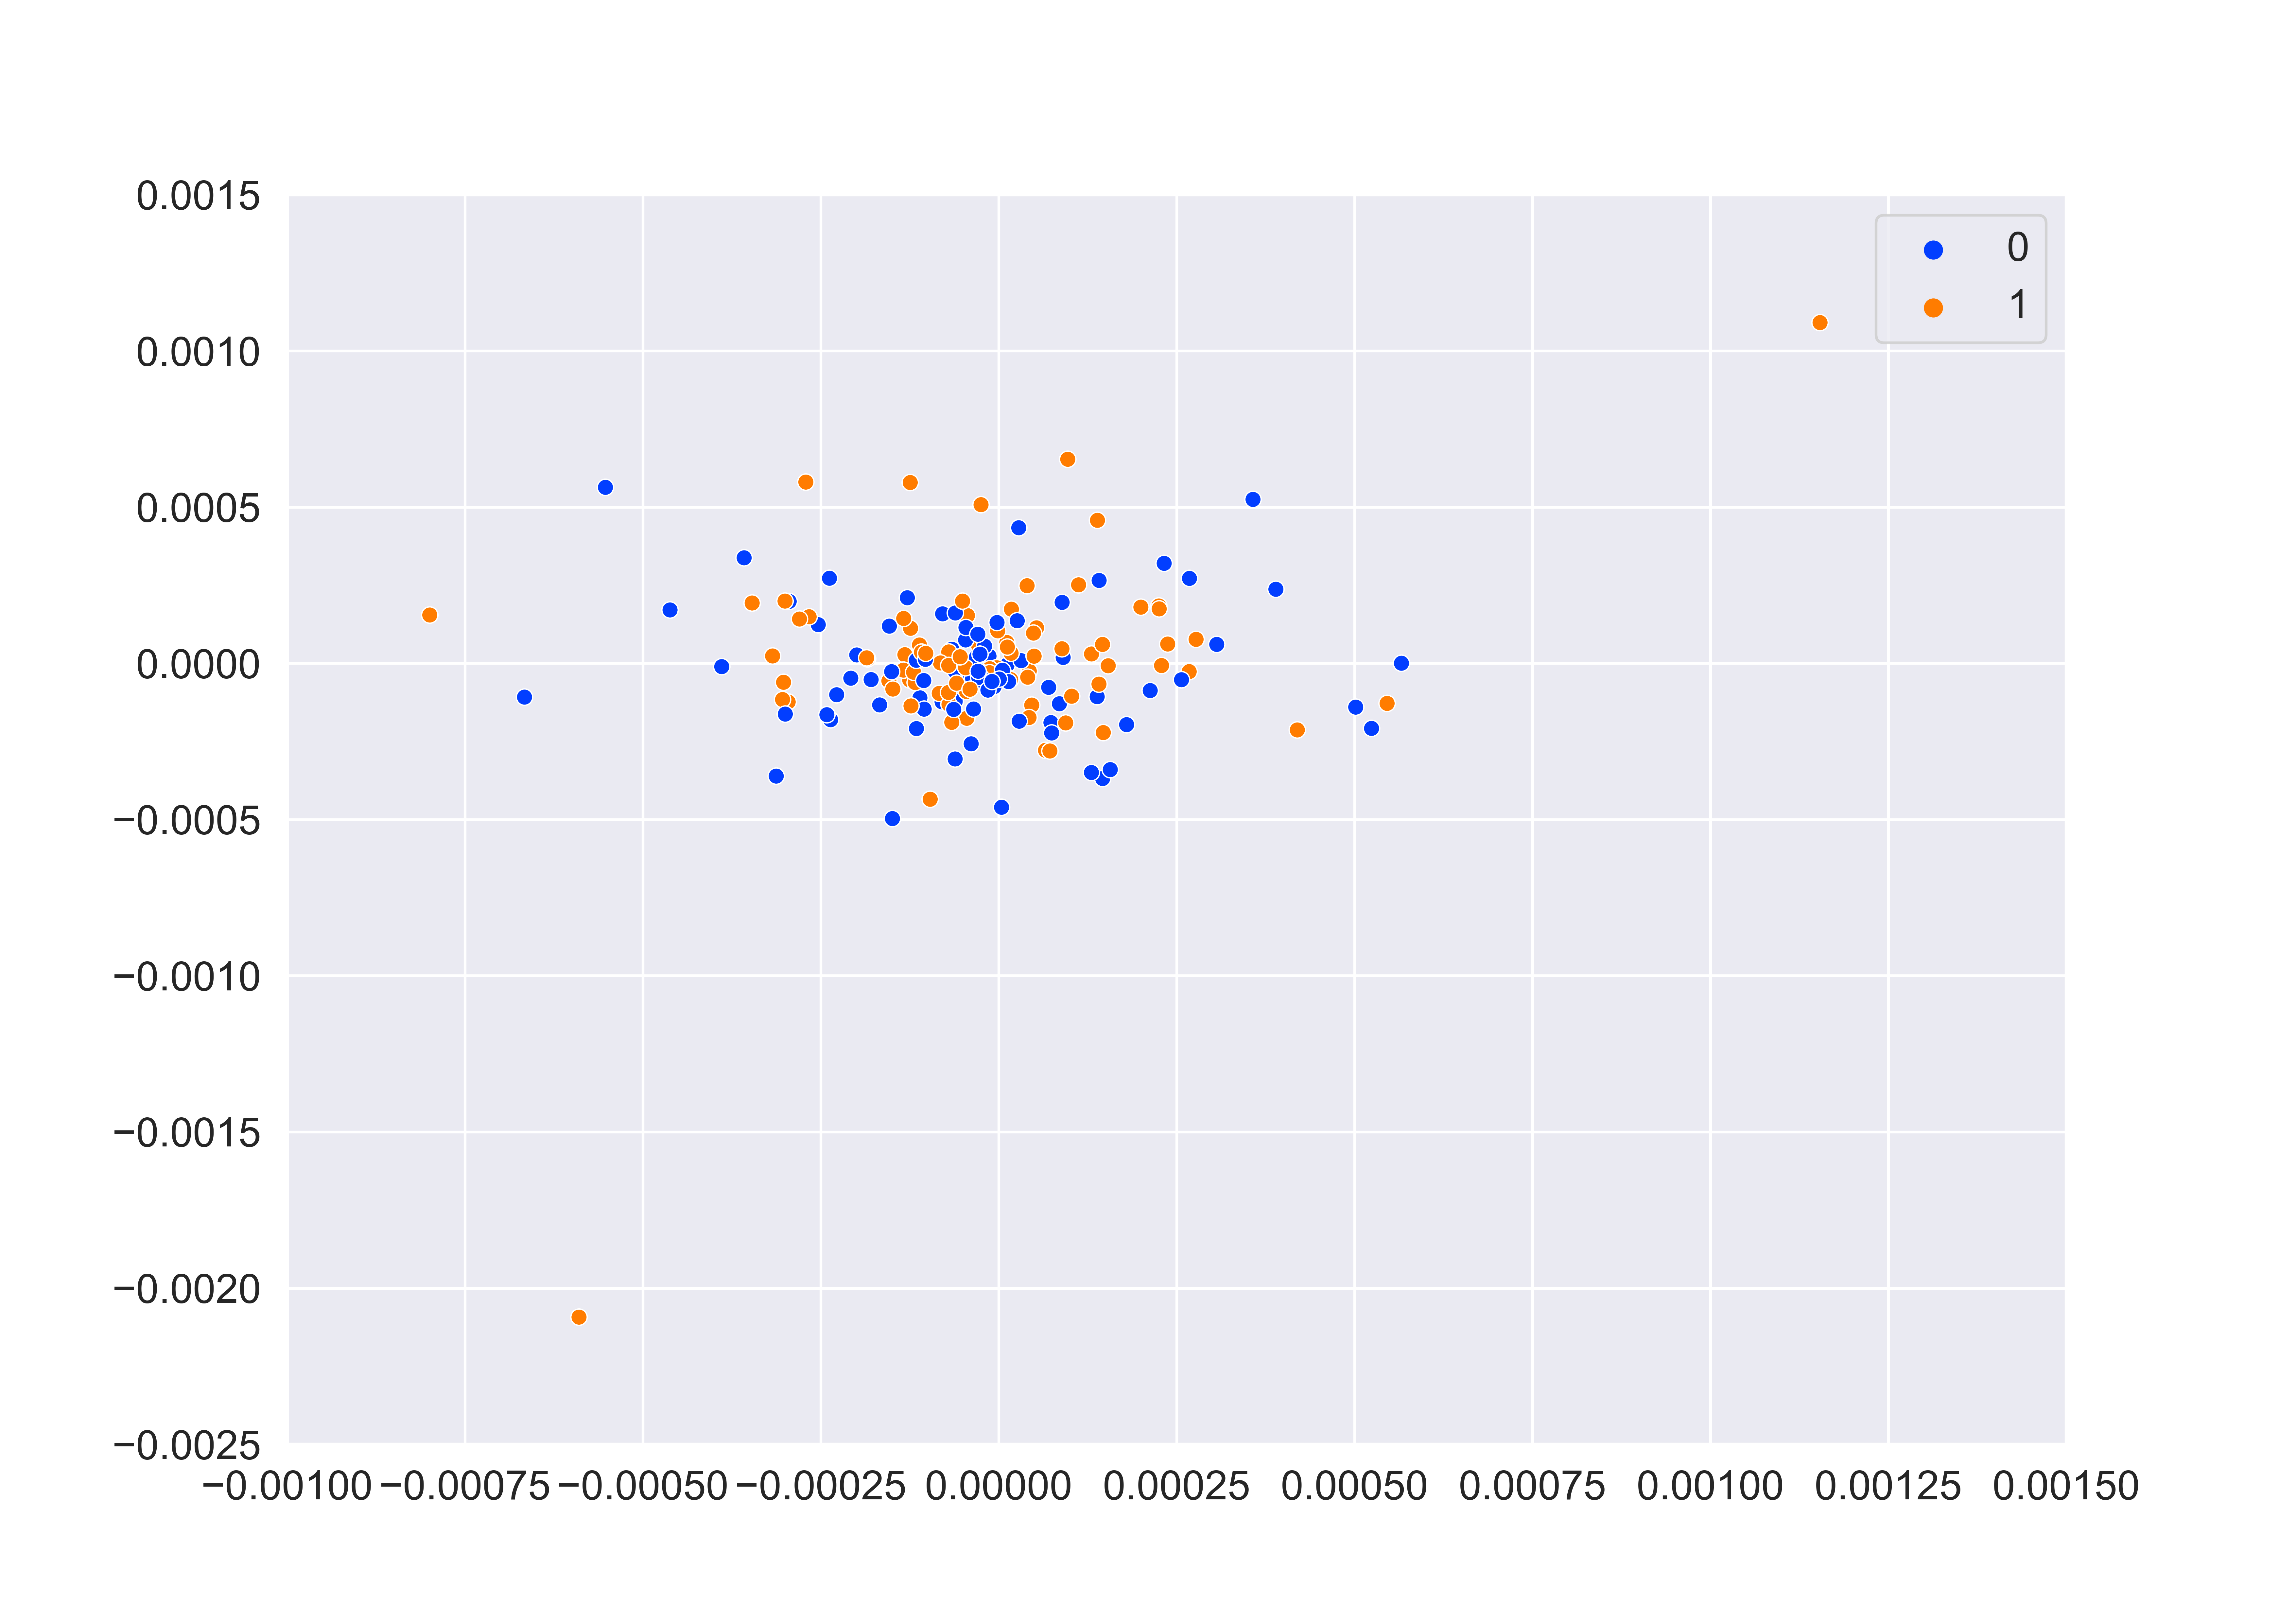
\includegraphics[width=0.45\linewidth]{../images/sst2_feature_map2_tsne.png}
        % \caption{Absolute value of indivisual components of weight in ridge regression when setting $\lambda$ to 1.0.}
        % \label{fig:mnist_tSNE_2}
    \end{subfigure}
    % \hfill 
    \begin{subfigure}
        \centering
        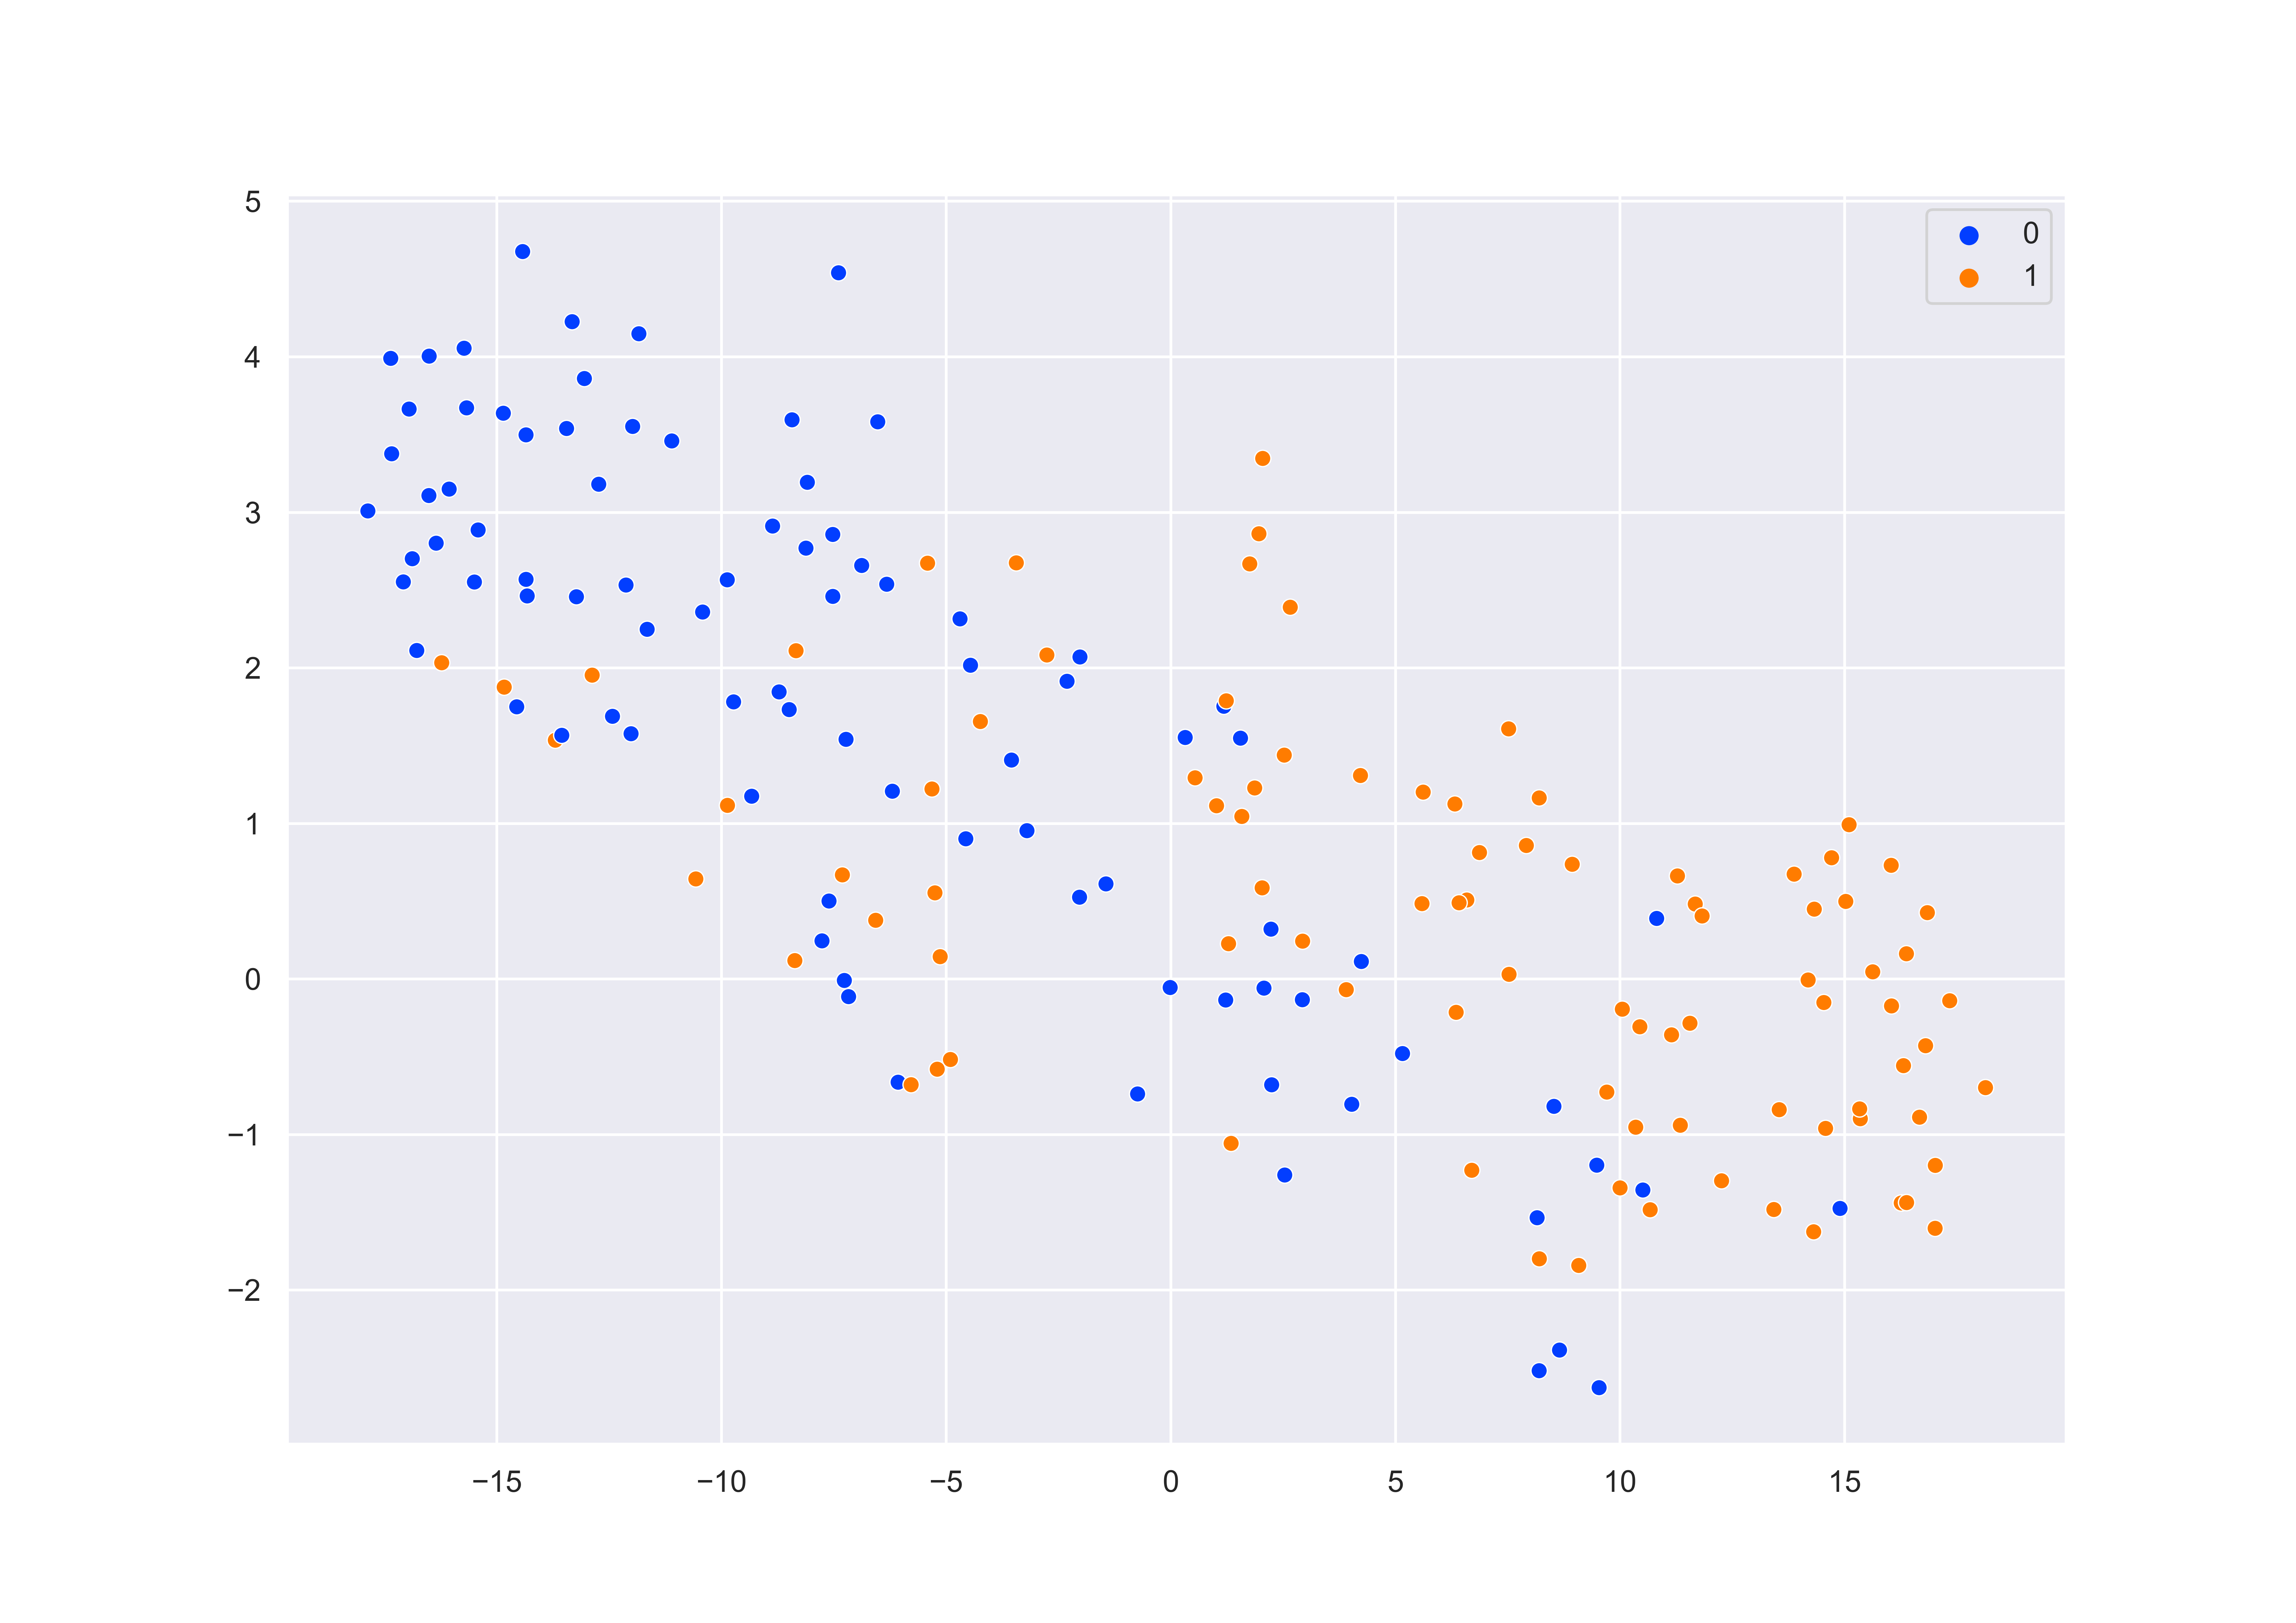
\includegraphics[width=0.45\linewidth]{../images/sst2_feature_map3_tsne.png}
        % \caption{Absolute value of indivisual components of weight in ridge regression when setting $\lambda$ to 1.5.}
        % \label{fig:mnist_tSNE_3}
    \end{subfigure}
    \begin{subfigure}
        \centering
        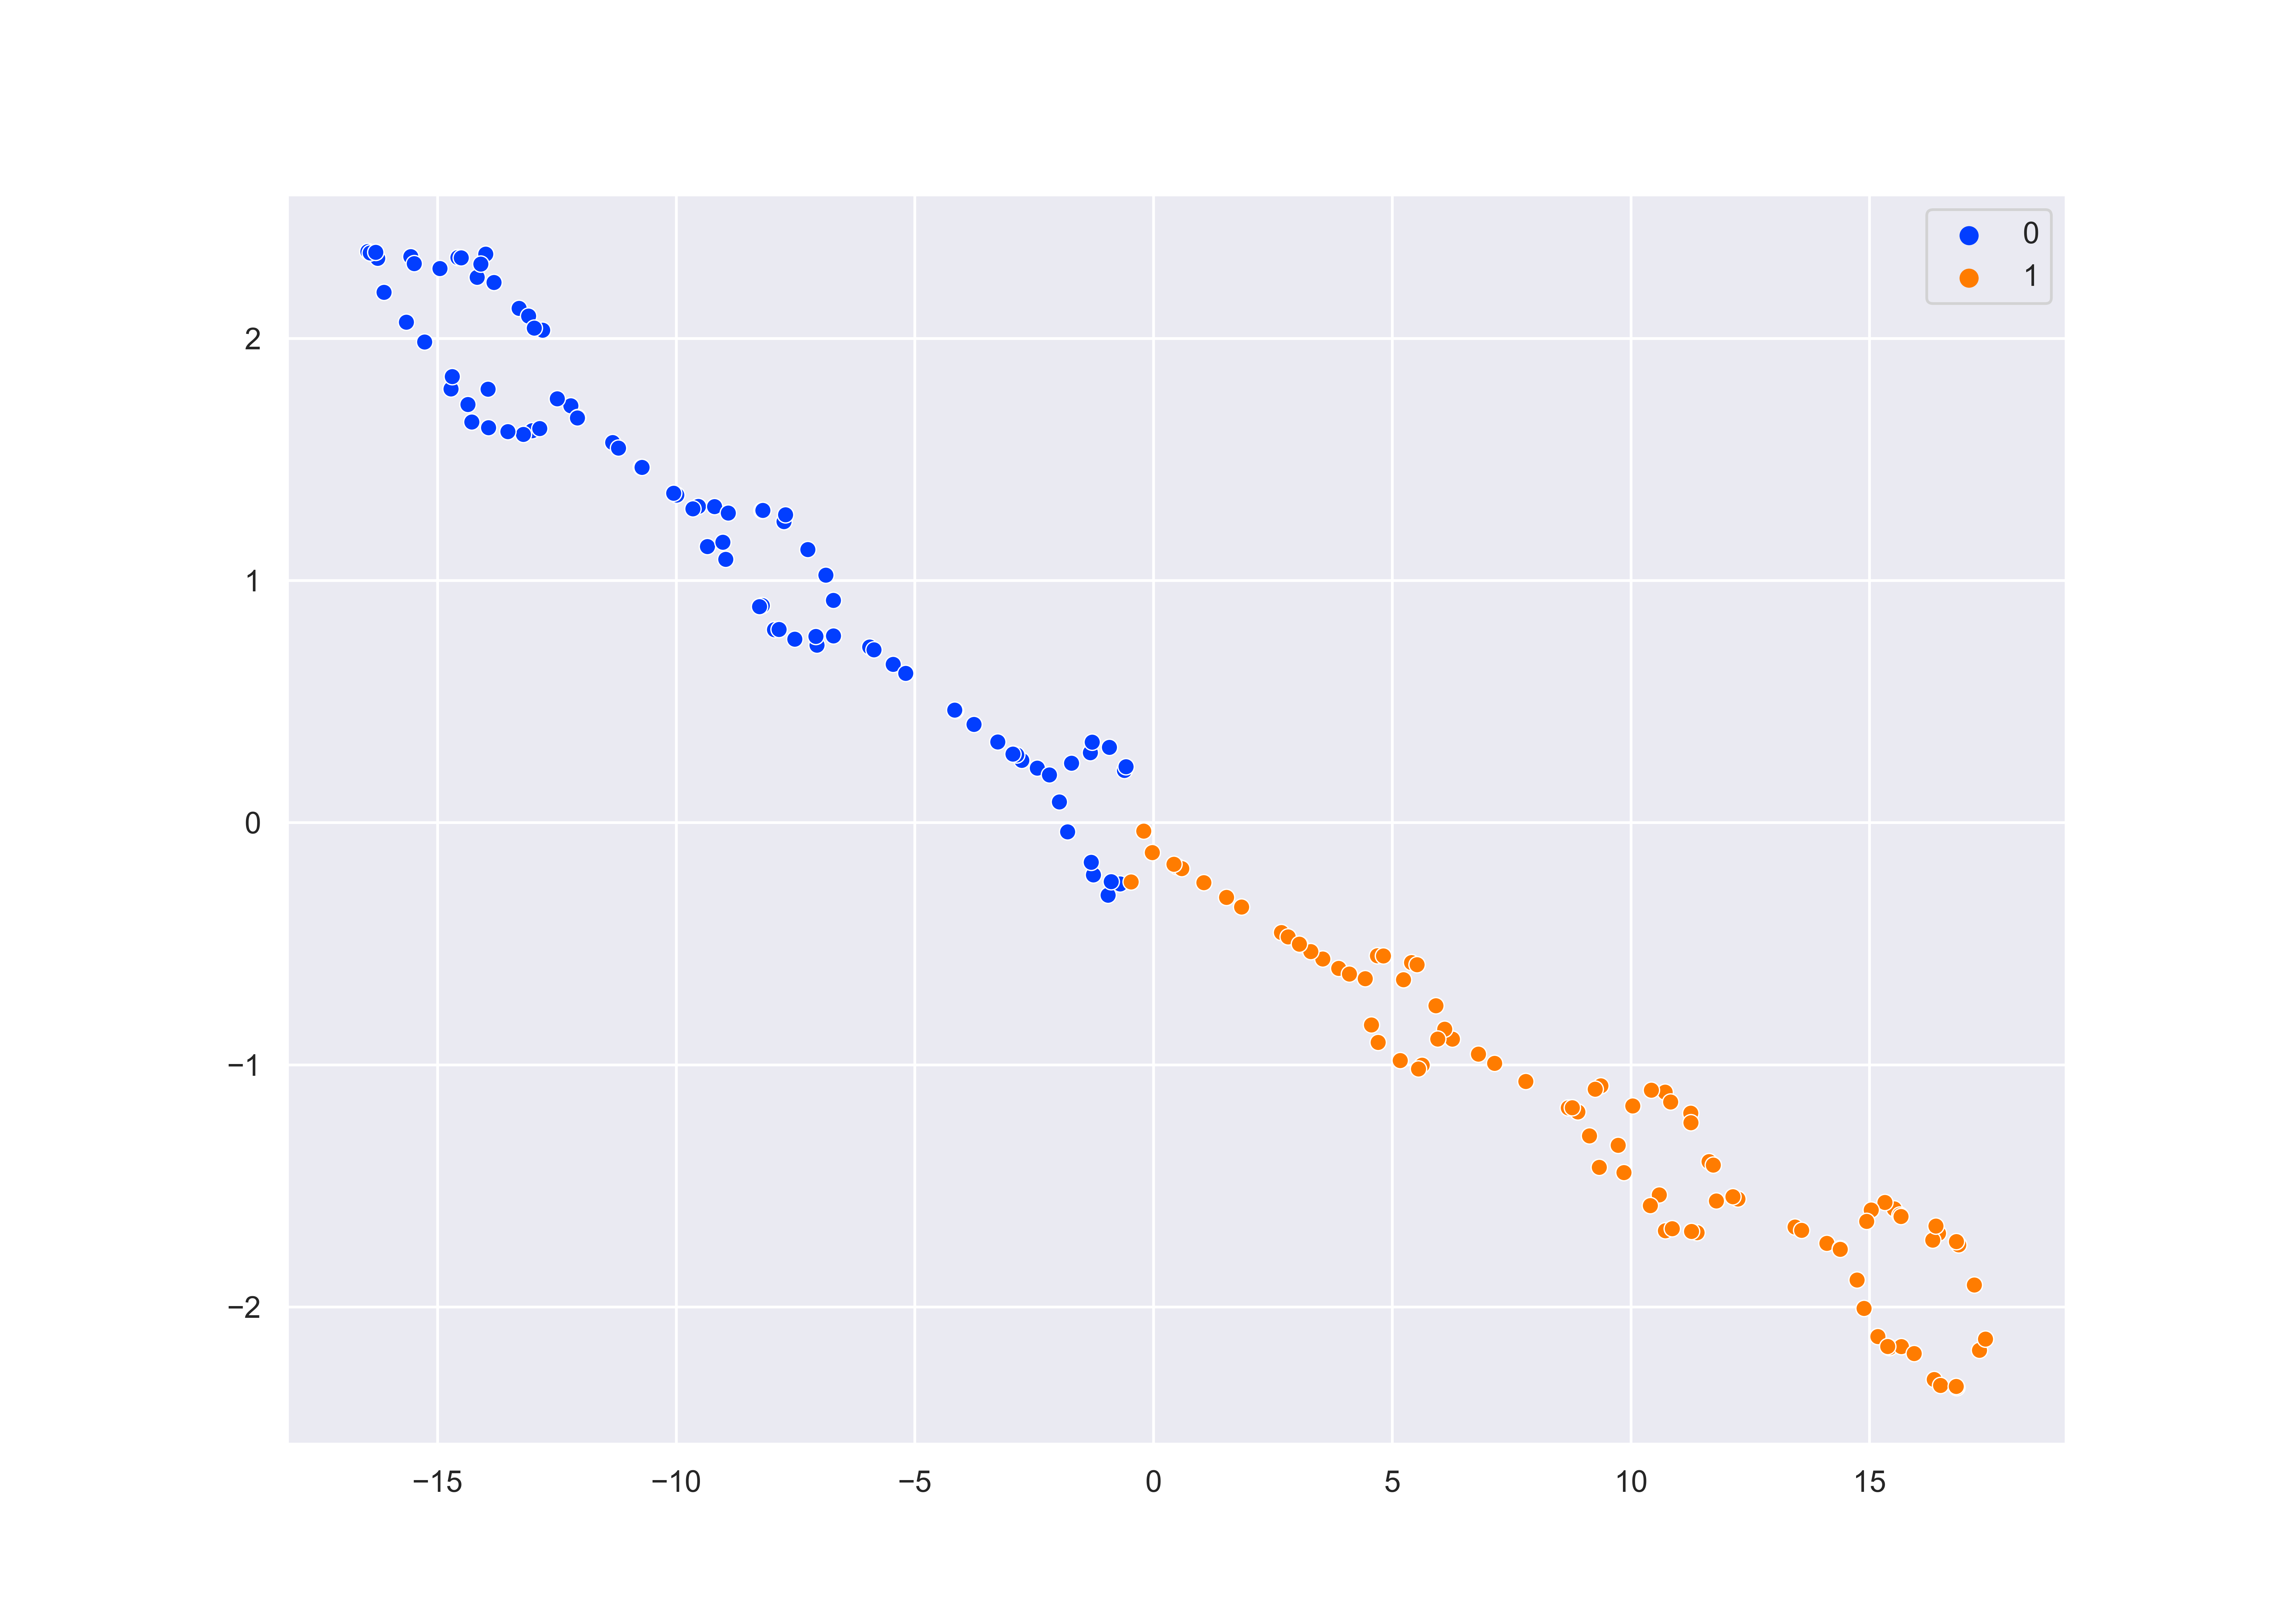
\includegraphics[width=0.45\linewidth]{../images/sst2_feature_map4_tsne.png}
        % \caption{Absolute value of indivisual components of weight in ridge regression when setting $\lambda$ to 1.5.}
        % \label{fig:mnist_tSNE_3}
    \end{subfigure}
    \caption{Visualization images of intermediate output tensors with t-SNE method. Top-Left: Tensors after the first LSTM layer. Top-Right: Tensors after the second LSTM layer. Bottom-Left: Tensors after the final LSTM layer. Bottom-Right: Tensors after the first linear layer.}
    \label{fig:sst_tsne}
\end{figure}

\subsection{Loss Function}
Again, in classification setting, I again add an additional logarithm operation after softmax function for stable computation. 
And I again use negative log-liklihood function defined in Eq.~\ref{eq:nllloss}, where $K=2$ in this setting.

\subsection{Experiment Result}
The training accuracy and validation accuracy are plotted in Fig.~\ref{fig:sst-train_loss} and Fig.~\ref{fig:sst-dev_loss}. 
The best checkpoint can achieve $68.64\%$ accuracy, which is on par with fine-trained LSTM models.
From training loss figure, the loss is smoothly decreasing, meaning that the learning rate is appropriate.
From validation loss figure, the validation loss is increasing but accuracy is also increasing in the first 10 epochs. 
After 10 epochs, the validation accuracy is fluctuating between $70\%$ and $72\%$.
So it verifies that if I need to tune the hyperparameters, I can lower down the learning rate after 10 epochs for better result.
But I do not choose to do so because tuning hyperparamters costs computational resources a lot and is meaningless in this task.
\newline
\newline
\noindent 
Besides, I sample the last token of each sentence after each LSTM layers and the tensor after the first linear layer for visualization.
Their corresponding visualization result is presented in Fig.~\ref{fig:sst_pca} with PCA method and Fig.~\ref{fig:sst_tsne} with t-SNE method, respectively.
It can be seen that at the beginning of the LSTM layers, my model cannot well distinguish the negative samples and positive samples well.
But after the final LSTM layer and the first linear layer, the datapoint can be separated well by my model, which again verifies the correctness of my LSTM model.

\subsection{Discussion}
The accuracy can be improved from two aspects. First, use pretrained word embedding for each word, such as word2vec or Bert-initialized word embedding. 
These word embeddings can assign more semantic information for one specific word, including the word itself and its neighbors.
The hidden state of each word can be more representative and further enhance the accuracy.
\newline
\newline
\noindent 
Second, I only consider one way, that is left-to-right information, while to predict the sentiment of a sentence, the former word can also count.
Therefore, the accuracy can be improved by adopting BiLSTM instead of vanilla LSTM.
\newline
\newline
\noindent 
Apart from improvable points, the stacked layers of LSTM may not count a lot. 
Maybe a 2-layer LSTM model can also achieve the same accuracy with less computational cost. 
Increase of parameters only make a different when the input is not sophisticated enough.




\newpage
\section{Appendix}
\label{code:tsne}
t-SNE Implementation. Only paste function names and anyone can refer to the source code for complete implementation.
\begin{lstlisting}

class MytSNE:
    def __init__(self, n_components=2, max_iter=1000, neighbors=30,
                 learning_rate=200, embed_scale=0.1, tol=1e-5) -> None:
        self.n_components=n_components
        self.max_iter = max_iter
        self.neighbors = neighbors
        self.learning_rate = learning_rate
        self.embed_scale = embed_scale
        self.tol = tol
    
    def fit_transform(self, X: np.ndarray):
        # Omit
        return Y

    def calc_matrix_P(self, X: np.ndarray):
        # Omit
        return P
    
    def calc_p(self, D: np.ndarray, entropy: float, iter_times=50):
        # Omit
        return P

    def calc_entropy(self, D: np.ndarray, beta: float):
        # Omit
        return H
    
    def calc_matrix_Q(self, Y: np.ndarray):
        # Omit
        return Q
    
    def calc_grad(self, P: np.ndarray, Q: np.ndarray, Y: np.ndarray):
        # Omit
        return grad

    def calc_loss(self, P: np.ndarray, Q: np.ndarray):
        kl_loss = np.sum(P * np.log(P / Q))
        return kl_loss
        
\end{lstlisting}

\end{document}
